%%%%%%%%%%%%%%%%%%%%%%%%%%%%%%%%%%%%%%%%%%%%%%%%%%%%%%%%%%%%%%%%%%%%%%%%%%%%%%%%%%%%%
% Machine Learning in Prediction
%
% 1. Linear Models
% 2. Polynomial Models
% 3. Neural Networks
% 4. Linear parameter-varying models
% 5. Adaptive nature using ISIS algorithm
% 
%%%%%%%%%%%%%%%%%%%%%%%%%%%%%%%%%%%%%%%%%%%%%%%%%%%%%%%%%%%%%%%%%%%%%%%%%%%%%%%%%%%

Cheap data storage and escalation of computational power allowed the world to enter a new age: the age of \textit{big data}. With vast amounts of data, previously in-viable and data hungry machine learning algorithms are now implementable.  The technology sector was the first group to be able to exploit this arcane technology to create tremendous value in applications ranging from targeted advertisements to self driving cars. The value was so great that the current top four companies in America by market capitalization are all technology companies (Microsoft, Apple, Amazon, and Facebook) as of 2019. As the technology sector's successes grow, other industries begin to catch a glimpse of the potential value creation in their own respective industries and initiate their own digital revolution. The ripples of success from the technology industry ultimately resulted in waves of capital investments into machine learning (ML) and artificial intelligence (AI) from all industries.

ML solutions promise to be cheaper, more accurate, and have online learning abilities compared to traditional methods.  Additionally, the solutions are promised to be easier to implement and will take less time to design; feed it data and it will learn, as they claim.  With this mentality, machine learning engineers and data scientists from technology companies attempted to conquer other industries, one industry being process control and chemical engineering. Unfortunately, their crusade fell short and their successes were few due to their lack of engineering knowledge and inability to identify large value gains.  Typically, projects in technology companies deal with very unambiguous information such as identifying location of objects or predicting the enjoyments of an individual based on previous articles they have read. However, process control typically generate time-series data and are often very ambiguous with data characteristics unique to the industry. Some characteristics include time delayed data, multi-modal data, unreliable data, highly noisy data, state transition dynamics data, and any combination of the prior.  Due to the increased complexity, data pre-processing for ML projects in the process control industry is mission critical and much more vigorous for successful applications.

Table \ref{tab:2MLApplications} shows some general machine learning applications for the process control industry. Currently, ML applications in the process industry can be broken down into prediction, monitoring, and control.  The field of prediction deals with mapping from certain inputs to desired outputs. An example would be building a soft sensor to predict for a state, $x_{m}$, that is expensive to measure.  By identifying states highly correlated to $x_{m}$, a multivariate soft sensor can be built to inexpensively predict the state in the future. In ML monitoring, the algorithms are tasked to monitor the process for anomalous activities. Here, an example would be applying a classification method to predict for failures in process equipment.  Lastly, ML control is concerned with the topics of adaptive, multivariate optimal control. Reinforcement learning is the typical ML algorithm for control.  

\begin{table}[h]
    \centering
    {\setstretch{1.2}
    \begin{tabular}{c|c|c}
    Prediction & Monitoring & Control \\ \hline
    Soft sensing & Anomaly detection & Supervisory control \\
    Forecasting  & Anomaly prediction & Regulatory control \\
    Operator education  & Alarm prioritization & Operator education \\
    Digital twin  & Alarm reduction & Multivariate control\\
    \end{tabular}}
    \caption{General applications for machine learning in the process control industry.}
    \label{tab:2MLApplications}
\end{table}

 Figure \ref{fig:02AICloud} shows a the machine learning architecture that is generic enough for implementation in all industrial plants. First, the industrial process (e.g. refinery, pipeline, reactor, etc.) sends raw sensor data into the cloud, where it is cleansed through data pre-processing methods.  Then, the filtered data is sent into different machine learning algorithms depending on the objective of the application and will output the desired values.  After a set time frame, all ML models will then be re-updated to learn the newest experiences. For computations requiring speedy outputs, portions of the ML code can also be pushed to the local devices using Microsoft Azure IoT edge devices. 

\begin{figure}[h]
    \centering
    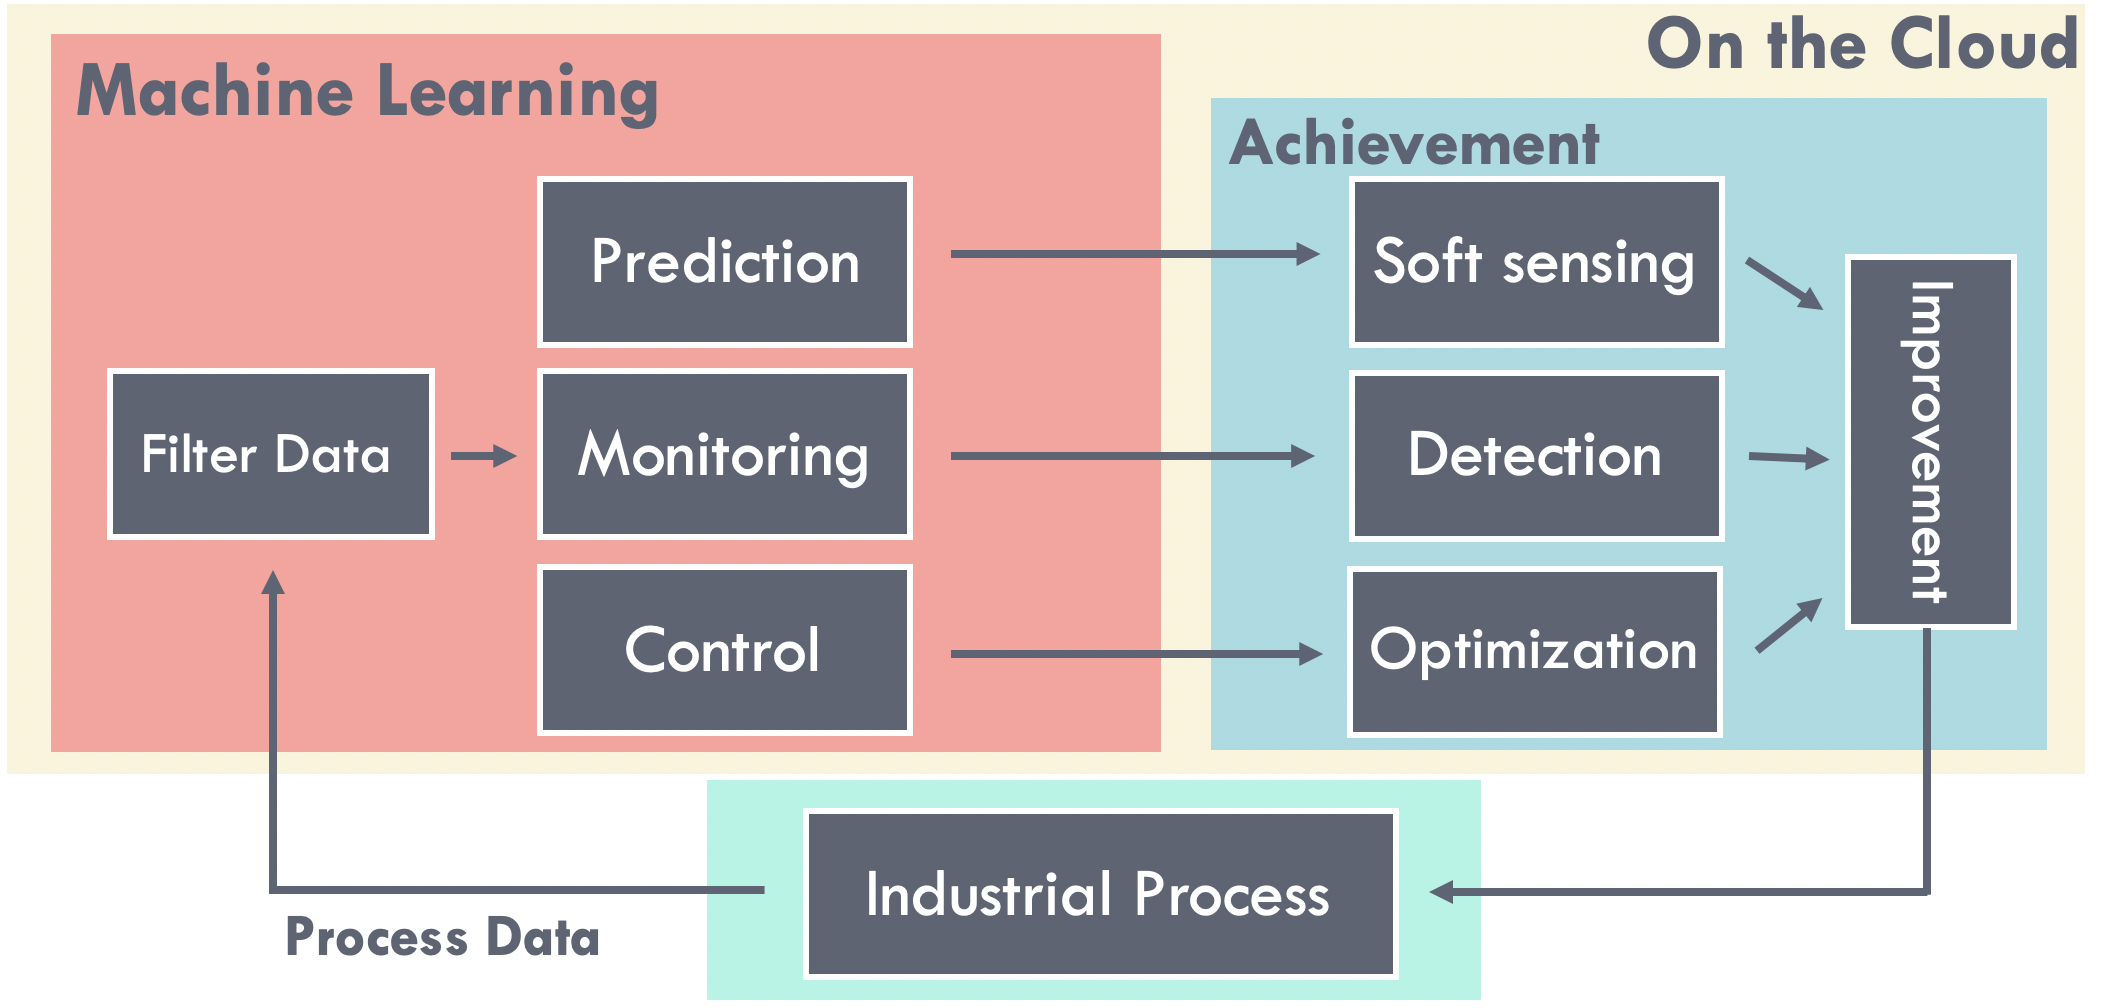
\includegraphics[width=\textwidth]{images/ch2/02AICloud.png}
    \caption{Overall machine learning architecture in an industrial environment}
    \label{fig:02AICloud}
\end{figure}

The objective of this chapter was to convey ideas for implementing machine learning solutions catered towards the \textbf{process control} industry.  In this chapter, the first half consists of common data pre-processing techniques to handle common process control concerns and is visually described by the "Filter Data" box.  The second half contains machine learning methods (in order of difficulty) to handle different process control prediction problems ("Prediction" box in the above figure). To conclude this chapter, the prediction algorithms will be closed off with an adaptive modelling technique inspired by reinforcement learning and adaptive resonance theory. For validation purposes, the machine learning methods were implemented onto an industrial pipeline for prediction, monitoring, and optimization\footnote{This project was supported in part by Mitacs through the Mitacs Accelerate program.}\footnote{This chapter only contains the theory and application highlights. The detailed industrial project report can be found in Appendix A.}.

Contributions made in this chapter include:
\begin{enumerate}
    \item Effective data pre-processing techniques for the process industry
    \item Catering machine learning prediction techniques to the process industry
    \item An outlier-free, data efficient, adaptive modelling method for multi-modal operations
\end{enumerate}

\section{Data Pre-processing}
Data pre-processing typically includes many steps starting with filtering by subject matter expertise, and then transitioning to common statistical methods.  For this section, only the filtering methods unique to process control will be discussed. Please refer to Appendix A for details regarding the other steps. Process control is typically concerned with multivariate time-series data plagued with noisy and/or unreliable sensor readings. Time delays are critical to successful prediction applications in process control. Furthermore, some processes may also have a variety of different operating regimes depending on downstream demand or ambient conditions.  In order to have successful prediction algorithms for process control, all of the above must be considered.

\subsection{Time Delay Data}
Time delay is the time between the performance of a control action and the change in output. Time delays occur due to the physics of the natural world.  For example, turning on a pump at the beginning of a pipeline does not result in higher flow rates immediately.  The process takes time to adjust and \textbf{transition} to the new steady state; therefore, raw data must be first shifted to account for the time delay.  Without doing so, models would be using current information to predict the past.  Imagine building a model to predict for the outlet flow rate of a pipeline where the regressors are pump statuses 300 km upstream of the outlet.  If a change in pump status occurred at $t = 0$, the pressure will take a few minutes to propagate down the pipeline.  Thus, the model taking pump statuses at $t = 0$ must have its flow rate labels shifted from $t = \tau$, where $\tau$ is the expected time delay.  An example of the time delay shifting procedure for an industrial pipeline is shown in Table \ref{tab:08TimeToCC} located in Appendix A, where data was shifted for different locations along the pipeline to enhance predictive capabilities.

Initial engineering expertise and/or data analysis must be conducted to identify the time delay for specific processes.  For example, it is well known that pressure propagates down incompressible fluids at approximately the speed of sound (1480 km/h) \cite{fluid_mechanics}.  Using this information, adjusting for the time delays along the pipeline was made trivial.

\subsection{Multi-modal Data}
In the process industry, it is common to have multiple modes of operation due to changing ambient conditions (e.g. summer, winter), different market demands, and a variety of other factors.  Each operating condition also consists of unique equipment operation and process characteristics (flow rates, temperatures, etc.); therefore, a common model to predict for many different operating conditions lead to increased model errors.  Here, unsupervised learning should be used to avoid this scenario for systems with many modes.  More specifically, clustering methods should be applied to segregate data from different operating modes, and separate models should be built using data from each operating mode to enhance accuracy.  For big data applications, \textit{k}-means or density based scanning (DBSCAN) should be used due to their scalability and non-iterative nature \cite{clustering_complexity}. Of the two methods, \textit{k}-means is much faster while DBSCAN is more robust to outliers.

An example of the breakdown of a multi-modal system can be found in Figure \ref{fig:08DBSCAN} in Appendix A.  By segregating the system into multiple modes, more accurate weights can be identified for each mode compared to general weights for all modes.  In fact, most modes would not even use the same equipment.  Such a concept is similar to using a linear parameter-varying model to approximate a non-linear system.  

\subsection{Unreliable and Noisy Data}
Thousands of measured data are recorded per minute on modern distributed control systems. However, many process variables such as viscosity, or parts per million (ppm) are difficult to measure with modern equipment on a live process. This results in inaccurate values being sent to the ML models, ultimately reducing accuracy.  To overcome highly unreliable data, a general strategy is to identify how the operator(s) are using the data and to engineer the feature(s) to be used in the same way for the ML model.  For example, the densitometers installed along the industrial pipeline shown in Appendix A all show different readings for the same crude. At times, the reading could be off by $\pm 20\%$. However, the operators only use the density reading to determine the grade of crude inside the batching pipeline. The crude is light if the API is above a threshold, heavy otherwise.  The physical number had no meaning for them.  To improve the ML model accuracy, the density reading was feature engineered to be a binary variable reading "1" if the API was above the threshold, "0" otherwise.  By doing so, the variable in the ML model was used in the same way as the operators and the accuracy increased.

Other data measurements may be accurate, but highly noisy. Noisy measurements may lead to significant predictive errors 
Noise can be reduced significantly by applying an exponentially weighted moving average (EWMA) filter given by:
\begin{equation}
    v_t = \beta v_{t - 1} + (1 - \beta) \theta_t, \; v_0 = 0
    \label{eq:08EWMA}
\end{equation}
\begin{equation}
    v_t \leftarrow \frac{v_t}{1 - \beta^t}, \forall v \in V
    \label{eq:08Bias_Correction}
\end{equation}
where $v_{t}$ is the exponentially weighted value at time $t$.  $\beta$ is the exponentially weighing factor.  Larger $\beta$ results in smoother results.  $\theta_t$ is the original value at time $t$. $V$ is a vector representing the exponentially weighted values before bias correction. EWMA is a very effective way to remove noise in chemical processes because these processes typically contain slow dynamics. By exponentially smoothing the data, the fast peaks are removed while preserving the slow dynamics. An example of the EWMA algorithm applied to the measurement of drag reducing agent (DRA) ppm values is shown in Figure \ref{fig:08DRA} in Appendix A.  DRA ppm measurements are known to be highly noisy; however, the noise can be almost completely removed by applying EWMA.

\subsection{State Transition Dynamics}
Another unique topic of process control is the dynamics of the system. System dynamics refer to the transitional period of going from one steady state to another after a control input is provided. Typically, dynamical models are used for advanced process controls where optimizing for the dynamics of the system is critical for optimal performance.  In order to build machine learning models to describe the dynamics of systems, a time-series implementation must be pursued.  Typical ML models map states and control actions at time $t$ to the desired output at time $t_{ss}$, where $t_{ss}$ is the time required for the system to transition to the new steady state.  By doing so, the dynamics of the system are completely omitted.  In order to build a dynamical ML model, the raw data needs to skip the time delay pre-processing step and be augmented by time.  Imagine a simple single-input single-output (SISO) system:
\begin{equation}
    y = w_1x + b
\end{equation}
In time-series implementation, the model would instead be:
\begin{equation}
    y_{t + 1} = w_1x_{t} + w_2x_{t - 1} + w_3x_{t - 2} + ... + y_{t} + y_{t - 1} + ... + b
    \label{eq:02_1step}
\end{equation}
where the input vector would be augmented as $\mathcal{X} = [x_{t} | x_{t - 1} | x_{t - 2} | ... ]$. Here, Equation \ref{eq:02_1step} becomes the 1-step ahead predictor of the system and dynamics can be predicted for. This data augmentation method is identical to all ML models if a time-series implementation is desired. In Appendix A, Figure \ref{fig:08ts_ls} shows an example of a time-series prediction model.  Because such models only predict one step in advance, error is typically very low.  The predicted value can also be fed in recursively to generate a infinite step ahead prediction that can be used for forecasting long term trends.

\section{Machine Learning Methods}

Many ML methods exist for prediction, each having its advantages and disadvantages. In this section, the most common ML methods will be shown along with their applications in process control.  Unique hyper parameters for different ML methods will also be shown; however, common hyper parameters such as $\alpha$, training epoch, and mini-batch size are common throughout and will be omitted.  Furthermore, common model performance metrics will be introduced. 

\subsubsection{Performance Assessment}
The model performance were assessed using the following three ways:
\begin{enumerate}
    \item Root mean squared error (RMSE) \cite{NN}:
    \begin{equation}
        J = \sqrt{\frac{1}{n}\sum\limits^n_{i=1}(\hat{y}_i - y_i)^2}
        \label{eq:08RMSE}
    \end{equation}
    
    \item Mean absolute error (MAE) \cite{NN}:
    \begin{equation}
        J = \frac{1}{n}\sum\limits^n_{i=1}|\hat{y}_i - y_i|
        \label{eq:08MSE_Error}
    \end{equation}
    \item Coefficient of determination ($R^2$) \cite{NN}:
    \begin{equation}
        R^2 = 1 - \frac{\sum\limits^n_{i = 1}(\hat{y_i} - y_i)^2}{\sum\limits^n_{i = 1}(y_i - \bar{y_i})^2}
    \end{equation}
\end{enumerate}
Table \ref{tab:02performanceassessment} shows the advantages and disadvantages of each assessment metric.
\begin{table}[h]
    \centering
    {\setstretch{1.2}
    \begin{tabular}{ c | p{6.2cm} | p{6.0cm}}
         Method             & Advantages        &  Disadvantages \\
        \hline
        RMSE                &  Useful for identifying large errors                            &  Smaller errors are muted        \\
        
        MAE                 &  Easy to interpret as all errors have the same weight           &  Inferior to RMSE when large errors are undesirable \\
        
        $R^2$               &  Easy to understand, {\small $-\infty \leq R^2 \leq 1$   }                                      &  Valid only for linear relationships       \\             
    \end{tabular}}
    \caption{Pros and cons of different model performance assessment methods.}
    \label{tab:02performanceassessment}
\end{table}


\subsection{Linear Models}
Linear models have two variants, linear regression and logistic regression.  The former is used for prediction tasks associated with continuous variables while the latter is used for classification tasks.  For example, linear regression is a great algorithm for soft sensor applications whereas logistic regression is more suitable for monitoring for anomalous activities. In this chapter, only the prediction variant will be shown. The model structure of linear regression is given as:
\begin{equation}
    \hat{y} = W_1^Tx + W_2^Tu + b
    \label{eq:02LS}
\end{equation}
where $x \in R^n$ is a vector of states, $u \in R^{m}$ is a vector of inputs and superscript $T$ denotes the transpose operation.  $\hat{y}$ is the predicted variable and can be anything; in soft sensors, $\hat{y}$ would be the "soft sensed" variable.  

The most common model structure for ML in the process control industry are linear models despite all processes being non-linear.  This is because the narrow region most processes operate around can typically be assumed to be linear \cite{process_control_ref13}.  Additionally, linear models are simple, interpretable, and require low amounts of data. However, the draw backs of linear models are their poor performance in the big data era where large amounts of data is available (see Figure \ref{fig:02learning_aggro}).  This trait is intensified given high dimensional data sets where identifying interaction effects are critical for accurate predictions.

Linear models were applied to the industrial pipeline as a benchmark algorithm.  The performance of the linear models can be seen in Tables \ref{tab:08LSperformance}, \ref{tab:08ConstLSPerformance} and Figures \ref{fig:08LSPlots}, and \ref{fig:08CLSPlots}. 

\begin{figure}
    \centering
    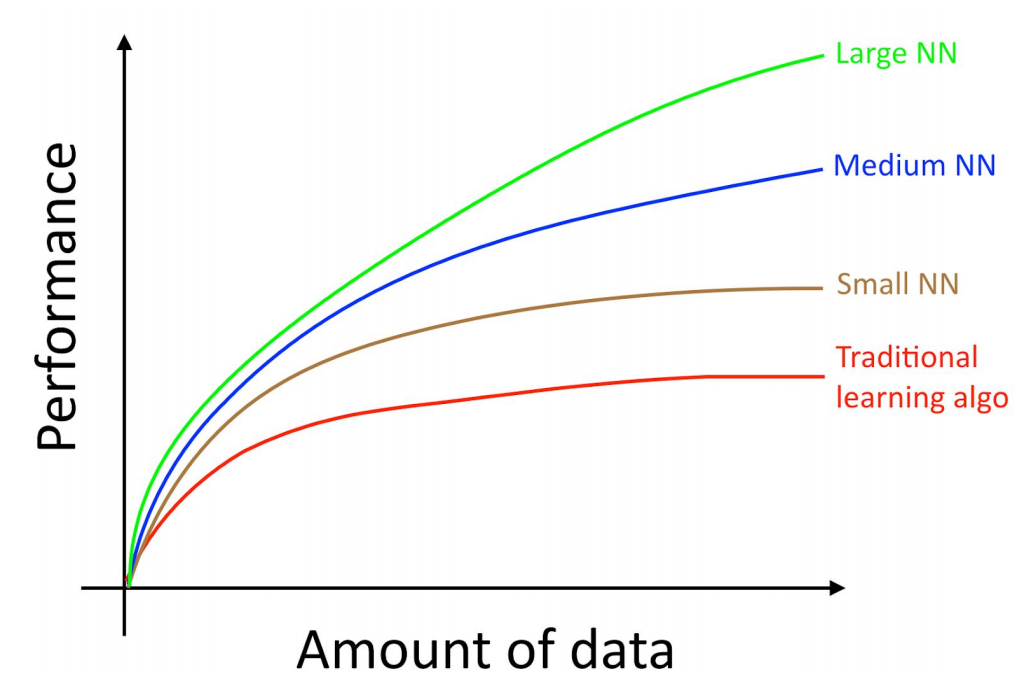
\includegraphics[width=0.7\textwidth]{images/ch2/02Learning_Aggro.png}
    \caption{Performance as a function of data.  Original image from \cite{deeplearning_course}.}
    \label{fig:02learning_aggro}
\end{figure}

\subsection{Polynomial Models}
Polynomial models are a general class of non-linear models that explores the main and interaction effects of its regressors.  The general model structure of a two regressor polynomial model is given by:
\begin{equation}
    \hat{y} = w_1x_1 + w_2x_2 + w_3x_1^2 + w_4x_2^2 + w_5x_1x_2 + e
\end{equation}
where $w$ are the weights, $x$ are the regressors, and $e$ is the modelling error.  In this model, linear, quadratic, and interaction effects are all explored simultaneously. However, the amount of parameterization required for a high dimensional prediction problem using this model structure might be difficult to interpret, thus, a truncated version of the model could be used instead for high dimensional problems. One special case of a truncated polynomial model is the exponential model given by:
\begin{equation}
    \hat{y} = w_1 x_1^{w_2} + b
\end{equation}
where the power of the regressor is also a weight to be identified. This is advantageous in situations where the non-linearity of the system is unknown. A quadratic and square root version of the exponential model were applied to the pipeline and the performances are shown in Table \ref{tab:08quad_sqrt_performance} and Figure \ref{fig:08PolynomialPlots}.  Compared to the linear models, the errors were reduced by up to 10\%.

\subsection{Neural Network and Deep Learning Approaches}
Neural network and deep learning approaches shine for predictive tasks where predictive power is the primary driver, while interpretability is not an issue, and acceptable\footnote{Neural network models are typically executed on servers and the outputs are sent to the actuators.  For fast processes, deep learning models should be pushed to the edge device.} hardware exists.  Deep learning is a special case of neural networks where many hidden layers exist.  The general consensus of the AI and ML community is that any neural network with more than three hidden layer is considered deep learning; however, the idea is not concrete and is open to personal preference.  The neural network model structure is highly non-linear and attempts to explore interaction effects of all regressors.  For a more detailed explanation on neural networks, the notation of its the variables, and its theory, please refer back to Chapter 1. Only a brief summary of the theory will be provided here. Due to the model complexity and high parameterization of neural networks, its predictive powers are unparalleled compared to other methods and can fit any function. In \cite{nn_fit}, the authors showed that:
\begin{framed}
\begin{quote}
There exists a two-layered neural network with ReLU activation functions and $2n+d$ weights that can represent any function on a sample of size $n$ in $d$ dimensions. 
\end{quote}
\end{framed}
Three distinct types of neural networks exist: i) Multilayer perceptrons (MLPs); ii) Recurrent neural networks (RNNs); iii) Convolutional neural networks (CNNs).

A visual representation of a MLP is shown in Figure \ref{fig:02MLP}.  MLPs (also known as feedforward neural networks) are the simplest and most common of the three.  In MLPs, the outputs of each neuron, $a_j^{[r]}$, is computed as:
\begin{equation}
    a_j^{[r]} = f(w_1x_1 + w_2x_2 + ... + w_mx_m + b)
\end{equation}
where the function, $f$, is non-linear and known as the \textit{activation function}.  The purpose of $f$ is to introduce non-linearity to the model; a critical addition because no process in the real world is linear.  In an intuitive sense, MLPs can be visualized as a brute force approach to identify the interaction effects of every regressor with each other. Due to the sheer number of parameterization, MLPs are very effective in predicting in-sample data points.  However, the models suffer tremendously during events where the testing data is significant different.  Large MLPs also tend to overfit; thus, it is critical to increase regularization as the MLP increases in size.

\begin{figure}[h]
    \centering
    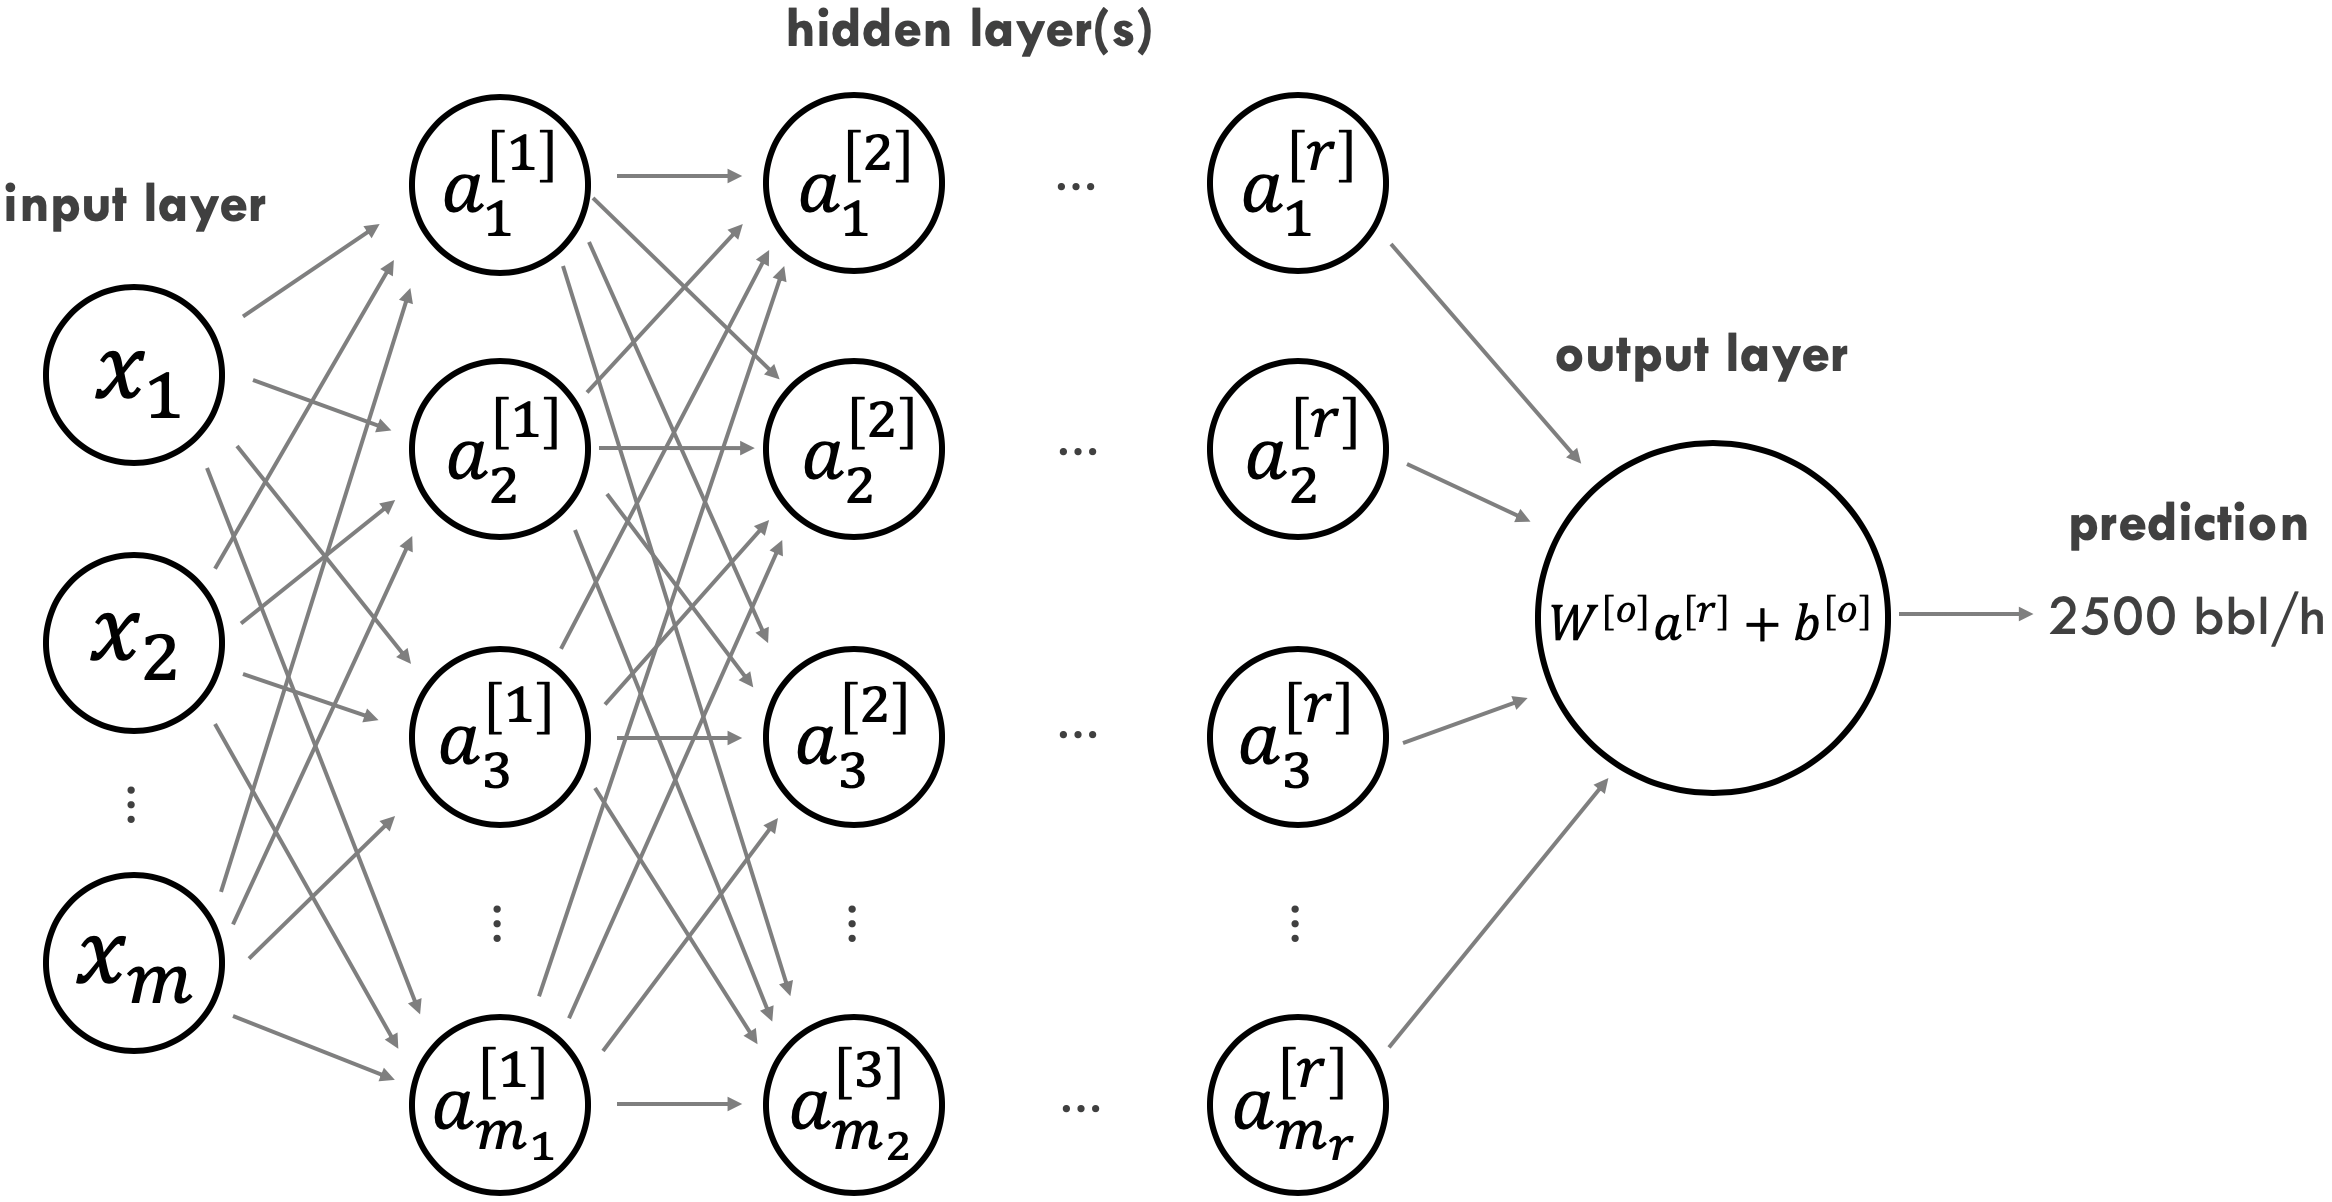
\includegraphics[width=0.9\textwidth]{images/suncor/08NN.png}
    \caption{Structure of a general neural network.}
    \label{fig:02MLP}
\end{figure}

MLPs were also applied to the industrial pipeline to model for the outlet flow rate. The input variables were measurements of variables along the pipeline such as temperatures and pressure, and the output was the outlet flow rate. Three different MLPs with varying sizes were applied.  Their respective performances can be seen in Table \ref{tab:08_nn} and Figure \ref{fig:08PolynomialPlots}.  It can be seen that the performance on the training and validation data were both excellent, though the error on the testing data increased significantly.  This was caused by the testing data being significantly different from the training data.  Data for model training was collected during the winter months, but was tested on summer months where the temperatures increased by up to $\ang{10}$ C. The increase in temperature resulted in reduced viscosity of the shipped crude and significantly hindered the predictive power of the MLPs. Ultimately, the MLPs' performance on the test data was almost identical to the much simpler polynomial models and was not used.

An especially useful type of neural networks for the process industry are RNNs (Figure \ref{fig:02RNN}) due to their time-series architecture.  Naturally, RNNs are set up to be infinite step ahead predictors and identifies temporal correlations within the data.  Traditional applications of RNNs can be found in speech recognition, translation, and language modelling.  In the process control industry where time-series data is abundant, RNN is the natural choice for typical soft sensing applications.  On a high level, RNNs accept inputs $x_t$, and outputs $y_t$.  At the same time, $y_t$ is sent as an input, along with $x_{t+1}$, back into the RNN to compute for $y_{t+1}$.  A similar computation is conducted until the end of the sequence of inputs.  By recursively re-inputting outputs as input data, RNNs are able to predict for an output trajectory given an input trajectory.

\begin{figure}[h]
    \centering
    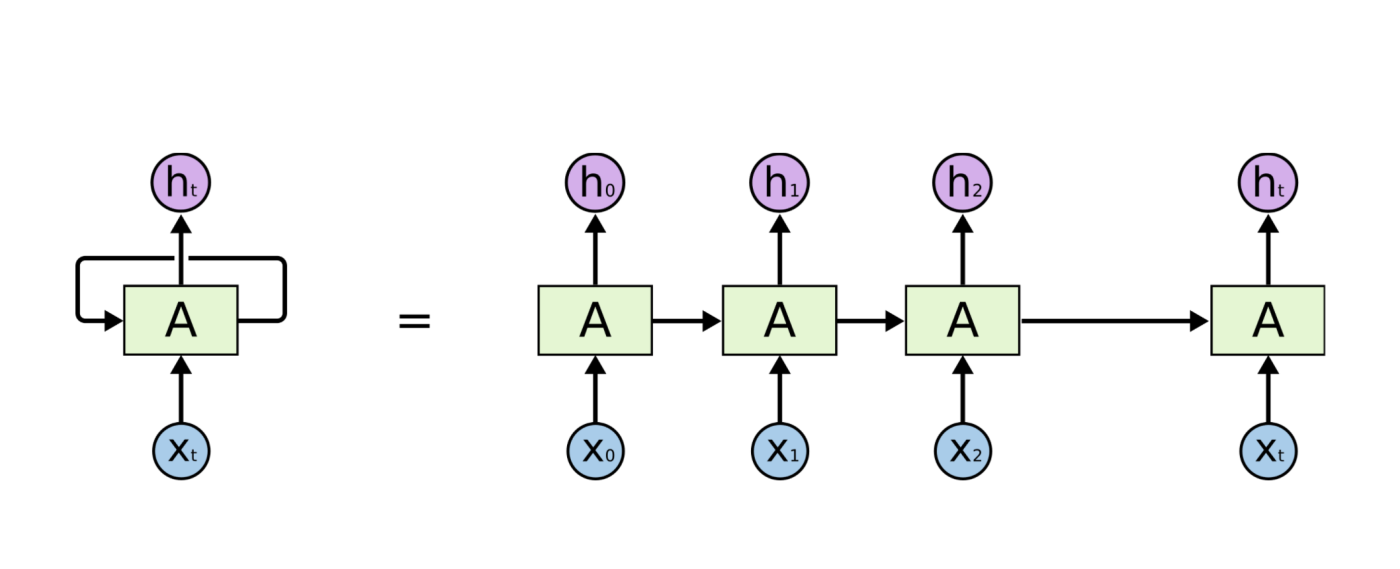
\includegraphics[width=0.9\textwidth]{images/ch2/02RNN.png}
    \caption{Architecture of a RNN.  Original image from \cite{NN}.}
    \label{fig:02RNN}
\end{figure}

CNNs are the last type of neural networks and are typically used for computer vision applications. The architecture of a typical CNN can be found in Figure \ref{fig:02CNN}. Unlike its predecessors, CNNs make the explicit assumption that inputs to the network will be images. This enables certain properties to be encoded into the architecture, making the forward pass more efficient while reducing the number of parameters.  More specifically, CNNs assume all inputs are arranged in three dimensions: height, width, and depth.  The height and width are simply the resolution of an image while the depth is the amount of color channels.  For example, a coloured image contains 3 channels (red, green, blue) while a grayscale image contains only one.  From this assumption, the weights of CNNs only need to be applied to specific locations, without the need of fully connected layers.  Furthermore, the input data will then be downsampled using pooling layers to extract the most important features while discarding the rest.  

\begin{figure}[h]
    \centering
    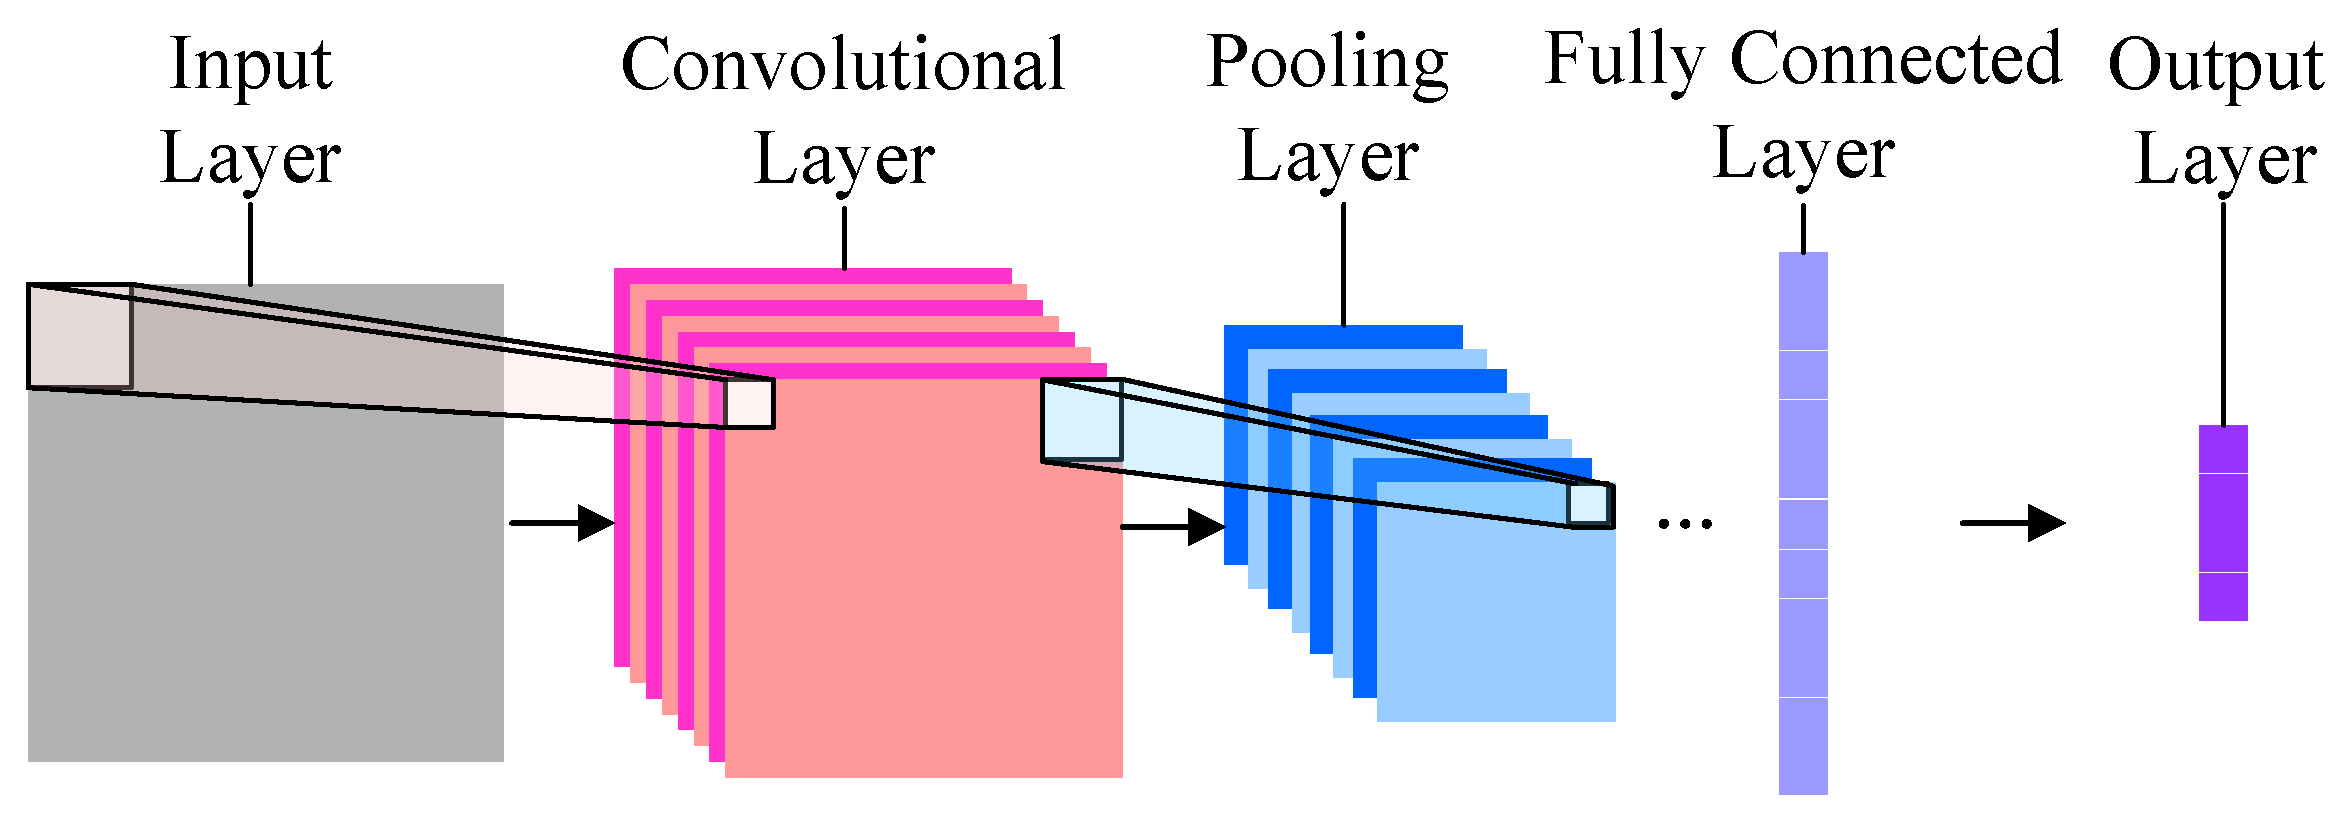
\includegraphics[width=0.9\textwidth]{images/ch2/02CNN.png}
    \caption{Architecture of a CNN.  Original image from \cite{NN}.}
    \label{fig:02CNN}
\end{figure}

In the process industry, CNNs can be leveraged as a soft sensor to measure variables using cameras. An example would be detecting the level of crude inside a primary separation vessel using the sight glasses, since traditional methods are not as effective.

Both CNNs and RNNs were not applied to the industrial project directly, but were provided to the reader as \textbf{advanced} methods for future projects that command exceptionally high predictive power, or computer vision soft sensing capabilities.  More information regarding RNNs and CNNs can be found in \cite{NN}.

\subsection{Linear Parameter-varying Models}
Linear parameter-varying models (LPV) were last type of ML models that were applied to the industrial pipeline. The motivation behind LPV models is twofold: i) Achieves a non-linear representation of the data using a combination of linear models; ii) Models different operating regimes of a process using different models.  The LPV model structure is identical to linear models with the exception that there are multiple linear models.  The number of linear models is a function of the non-linearity of the system, the number of operating regimes, and the amount of available data.  

Figure \ref{fig:02LPVexample} shows an example of fitting multiple linear models to approximate a non-linear system. Two separate approaches were used: 3-model approach and 6-model approach.  Performance wise, the 6-model approach is far superior. However, the 6-model approach uses twice as many models resulting in a significantly higher maintenance and ownership cost.  Additionally, the individual model performance for the 6-model approach may experience high variance if low amounts of data are present at certain points.  If performance is of utmost importance and data is abundant, a large number of linear models could be used.  Otherwise, a LPV model with a lower amount of models is adequate.

\begin{figure}[h]
    \centering
    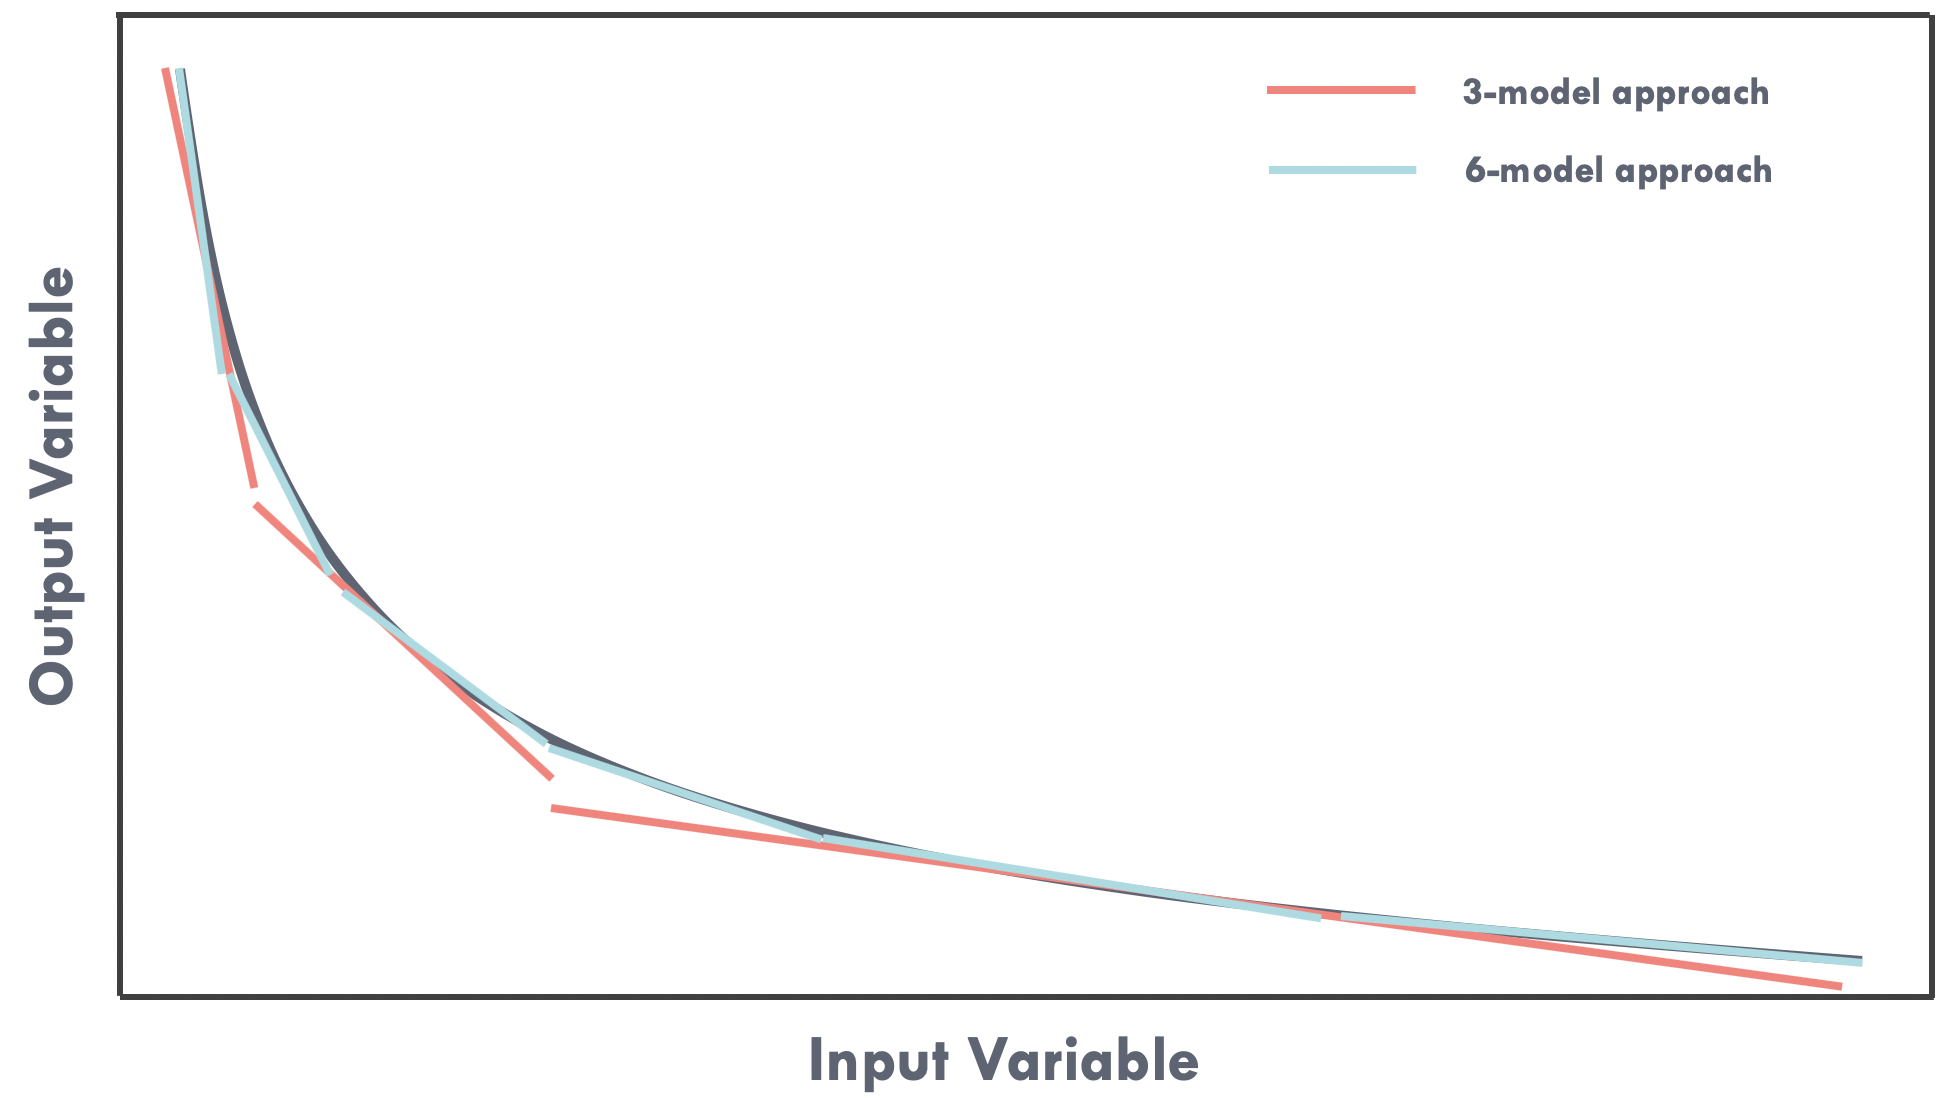
\includegraphics[width=\textwidth]{images/ch2/02LPVexample.jpeg}
    \caption{Fitting a non-linear function using multiple linear models.}
    \label{fig:02LPVexample}
\end{figure}

Clustering techniques can be used to identify distinct models for large MIMO systems containing multiple operating regimes and/or where non-linearity is not easily visualized.  Table \ref{tab:08cluster1_cluster2_reg} and Figure \ref{fig:08LPVModels} shows the application of a 2-model LPV model onto the industrial pipeline for the two separate operating regimes.  The original data set was first segregated into two clusters using DBSCAN.  Then, separate linear models were built for each cluster. During model testing, the Euclidean distance of new samples to the centroids of each cluster is computed to determine which linear model should be used for prediction. In terms of performance, the LPV model was able to achieve very similar performance metrics compared to the other non-linear models.  Additionally, the LPV models are more representative of the process in terms of control because each model (for each operating regime) has unique weights and constraints. For control, this is especially beneficial.  For example, if pump A was never used for operating regime B, the model would be highly inaccurate if the control system recommended its operation.  Using LPV models, explicit constraints can be placed to prevent such a scenario, as shown in the LPV section in Appendix A.

The training and deployment procedure for using a LPV model in an arbitrary process is shown in Figure \ref{fig:02lpv_architecture}.  Starting from the top, historical data for the process is first clustered into $n$ data sets.  Here, $n$ can be pre-defined using subject matter knowledge, or can be found using DBSCAN.  After segregation, each cluster should have enough data to effectively identify useful linear models.  Finally, the data sets are used to identify linear models.  Each model will have unique constraints to enhance the representation of the physical process.  Deployment-wise, new measurements are obtained from field sensors and are sent to the LPV model.  Then, the Euclidean distance (or desired distance metric) between the new measurement and the centroids of each model are calculated. The model exhibiting the lowest distance will be used for prediction. However, if the distance between the new measurement and the closest centroid is too large, the measurement will be labeled as anomalous instead.

\begin{figure}[h]
    \centering
    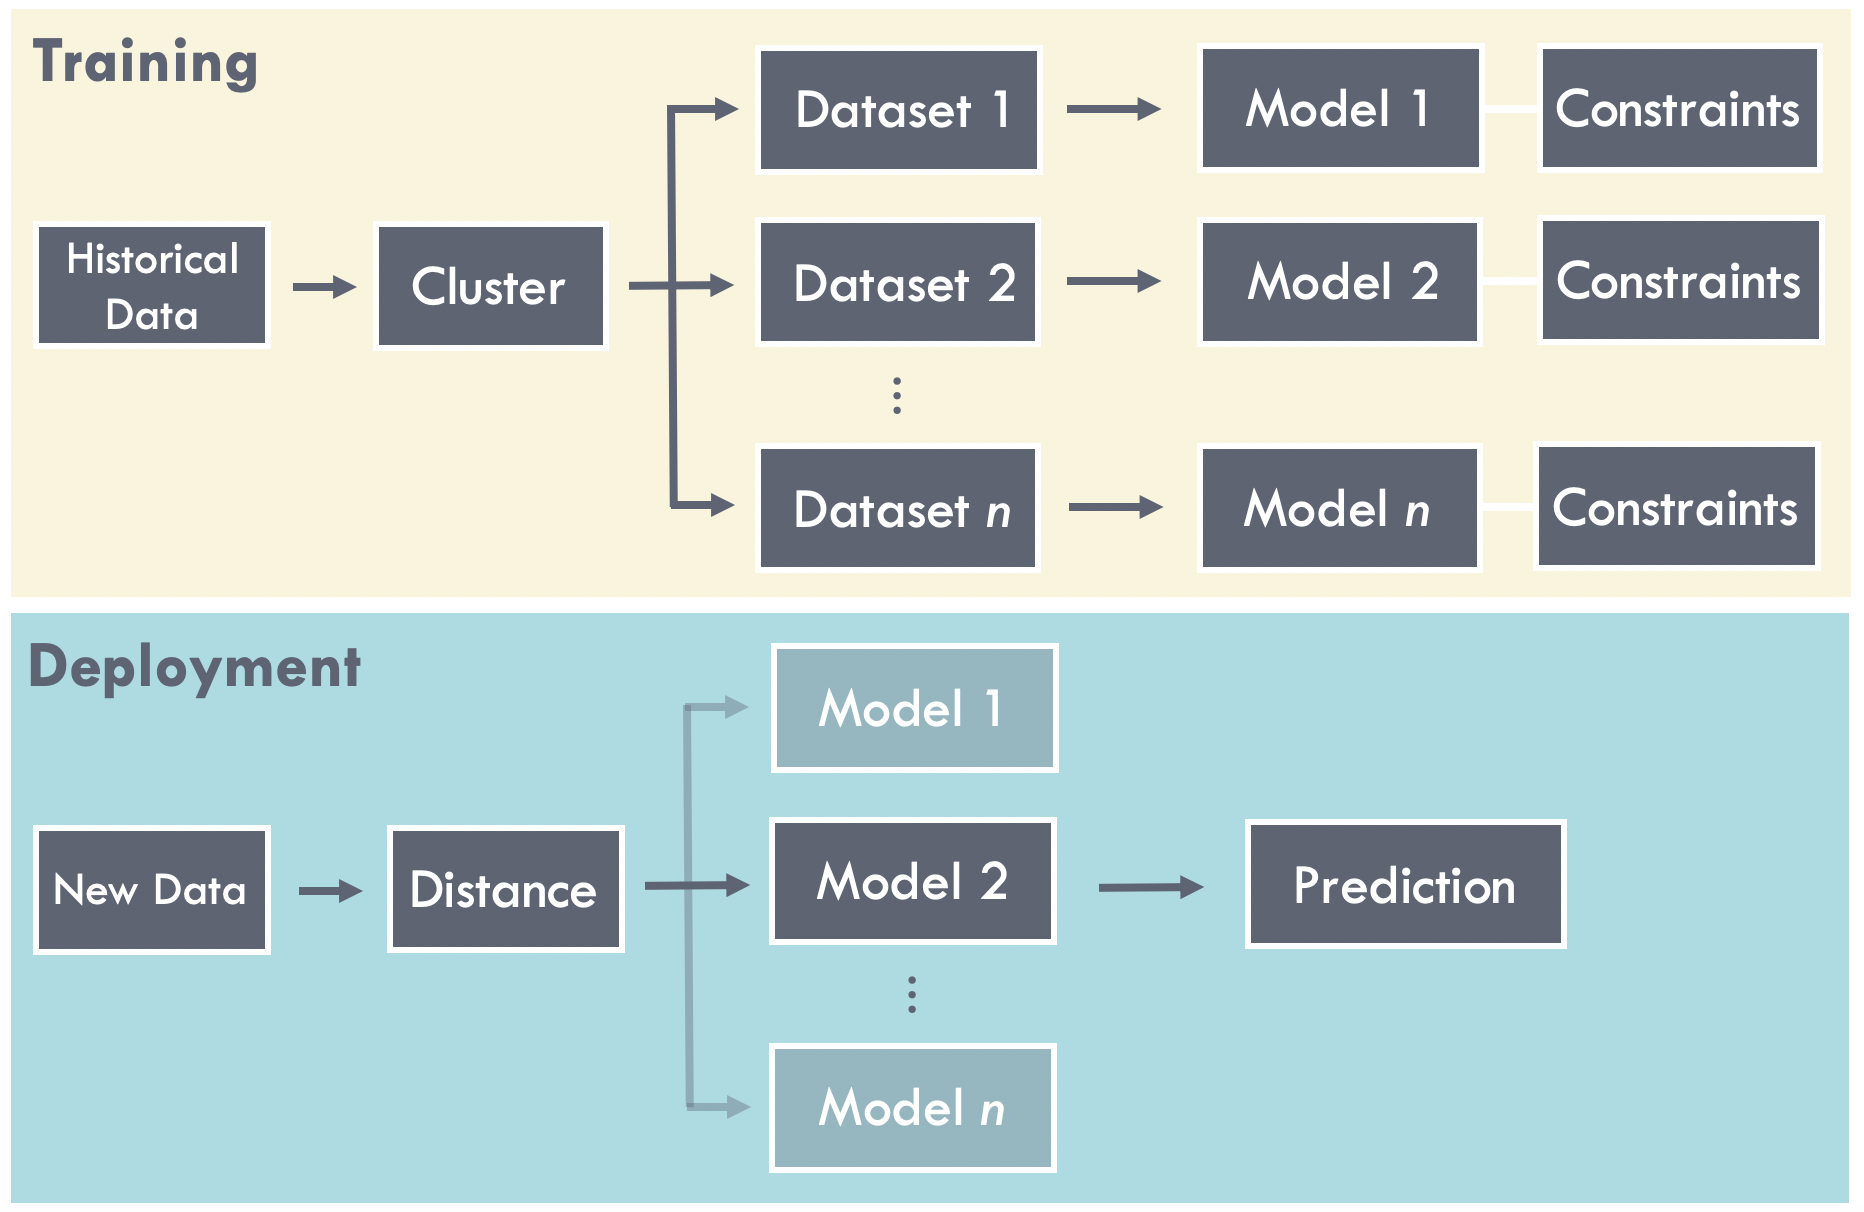
\includegraphics[width=\textwidth]{images/ch2/02lpv_architecture.jpeg}
    \caption{Architecture of the LPV model during training and implementation}
    \label{fig:02lpv_architecture}
\end{figure}

\subsection{USIS: Uniform Sampling Incremental Supervised learning}
A major selling point of ML solutions is their promise of being adaptive. Because of the way ML solutions are updated (gradient descent), adaption can easily be incorporated in a natural and biological way. Figure \ref{fig:02GradDesc} shows an intuitive representation of the gradient descent algorithm.

\begin{figure}[h]
    \centering
    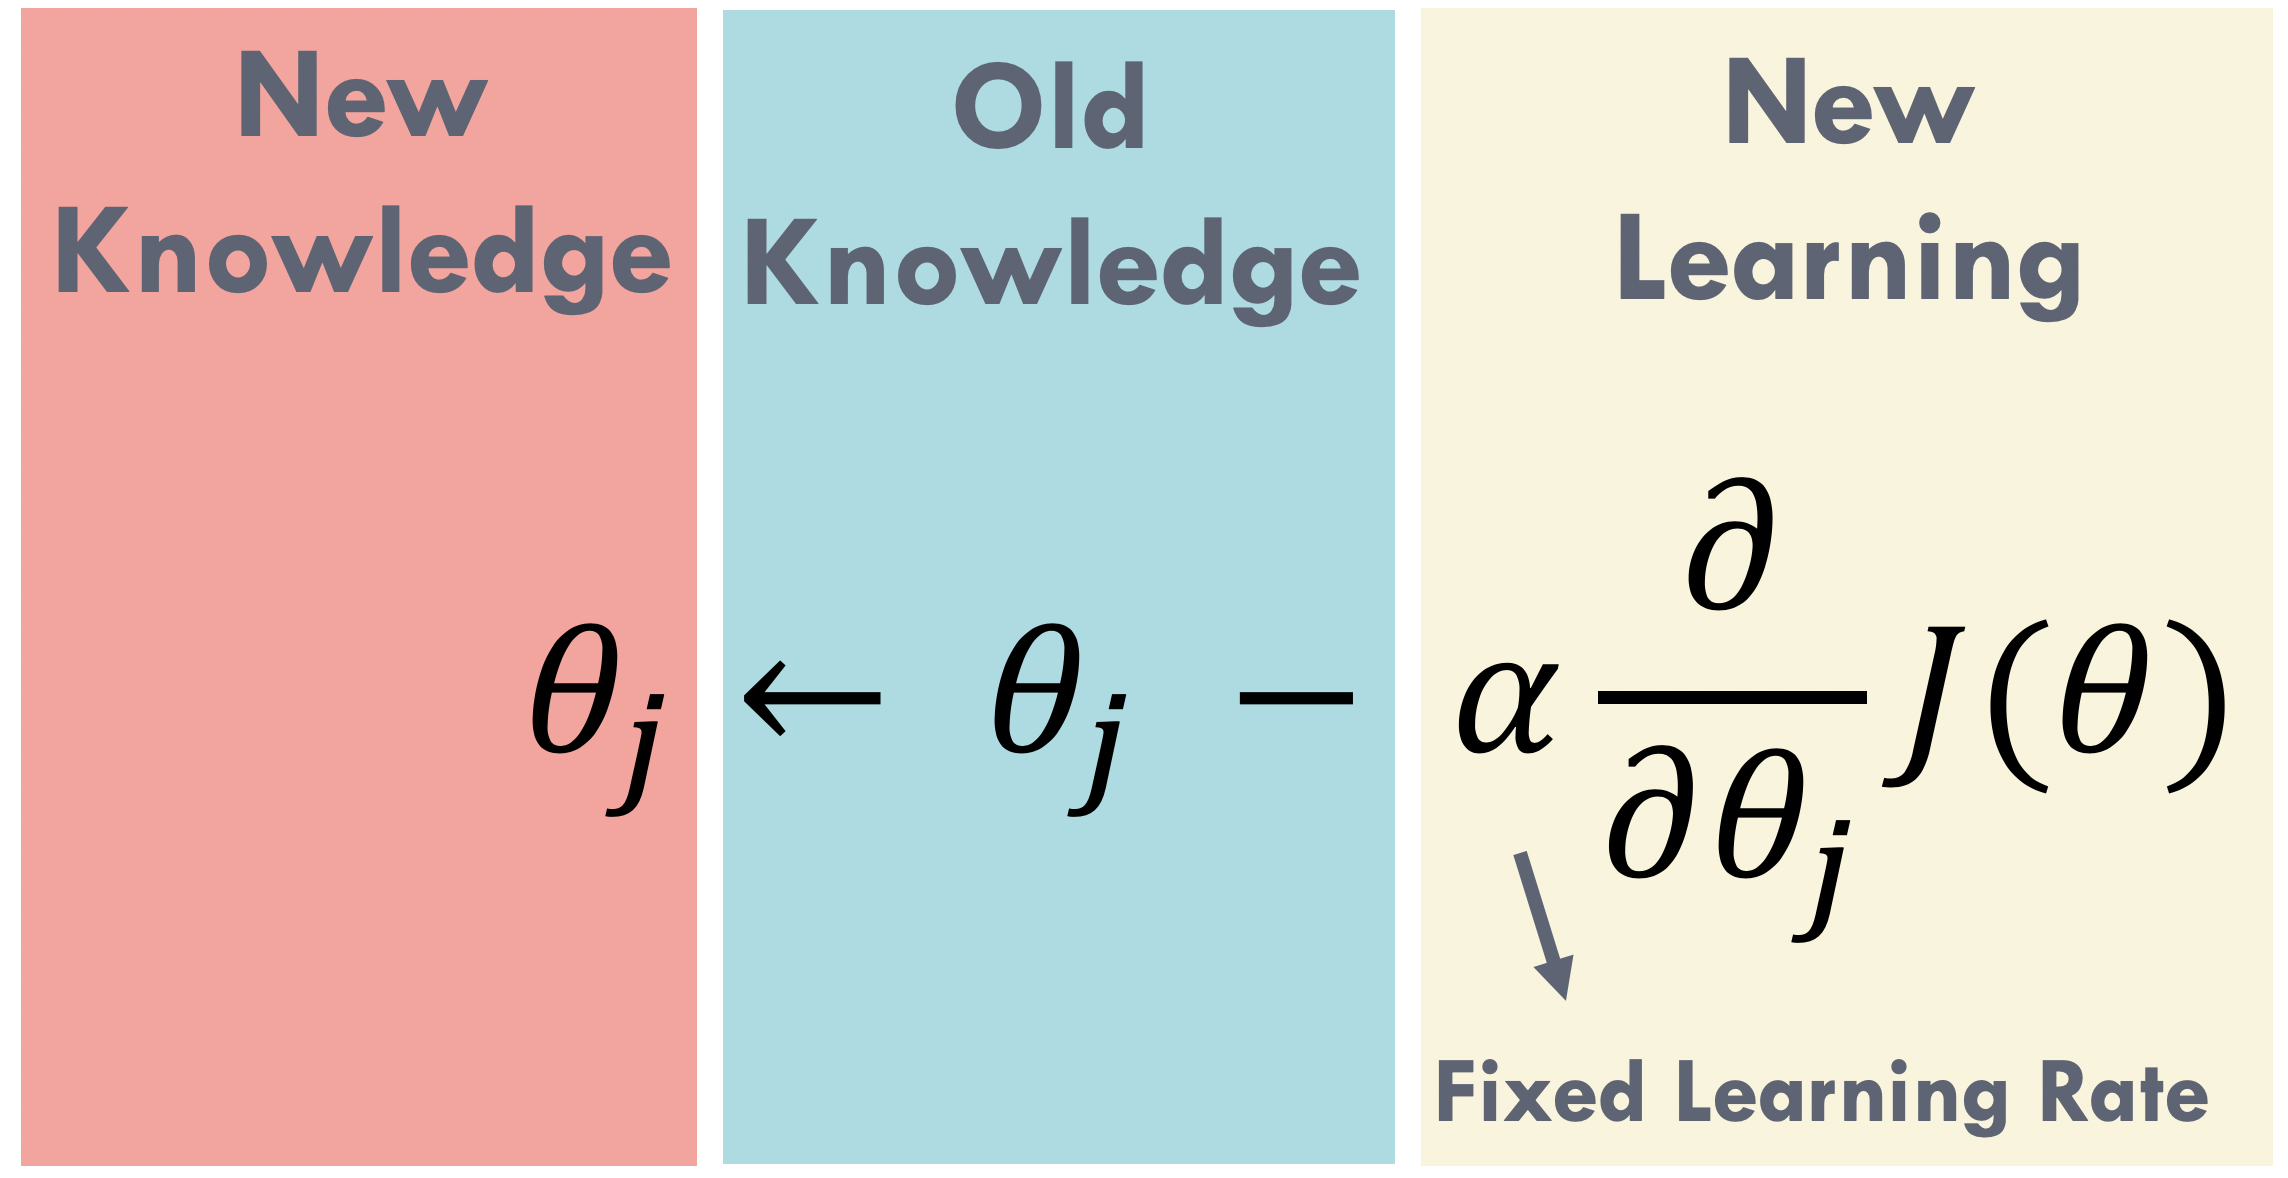
\includegraphics[width=0.75\textwidth]{images/ch2/02GradDesc}
    \caption{An intuitive representation of gradient descent.}
    \label{fig:02GradDesc}
\end{figure}

During an update step, the new knowledge is intuitively the old knowledge adjusted by new learnings.  The new learnings are typically multiplied by a fixed learning rate, $\alpha$. From this, the new knowledge is always biased towards the most recent experience, giving ML solutions an adaptive characteristic.  Adaptive ML can be implemented in two forms: online learning or incremental learning. Online learning refers to the ML models being updated after each prediction and can be understood mathematically as stochastic optimization. Common applications of online learning can be found in search optimization for web pages, where millions of data points are generated per minute. Online learning is not suitable for process control applications due to three reasons: catastrophic interference (i.e., tendency of neural networks to completely and abruptly forget previously learned information upon learning new information \cite{cat_int}), sequential noisy data decimating model accuracy, and insufficient incoming data to identify representative models for useful applications.  In adaptive ML, incremental learning is the preferred choice for process control applications due to its reduced randomness.  Incremental ML works by creating a data cache, and then updating the model using all data from the cache simultaneously after a fixed interval.  By doing so, the models will be updated much slower and the gradient of the loss function is an average of many examples, a method similar to semi-stochastic optimization.

\subsubsection{Motivation}
Incremental learning still falls short in terms of catastrophic interference (also known as catastrophic forgetting). This is especially a problem for the process industry, where operating conditions may be prolonged for many months before a switch is made. Because ML solutions are biased towards the most recent experiences, past experiences will be forgotten and the model will perform poorly if faced with old conditions after a long time. 

The uniform sampling incremental supervised learning (USIS) algorithm was proposed to overcome this issue and to enhance data efficiency for adaptive ML techniques.  USIS is a combination of adaptive resonance theory, uniform sampling, and experience replay (from reinforcement learning theory), where each update step is outlier free, data is efficiently used many times, and data is uniformly sampled across the distribution of the model to prevent catastrophic interference.

The simplified adaptive resonance theory (ART) architecture is shown in Figure \ref{fig:02art}. ART was originally proposed to prevent disrupting existing knowledge during learning of new knowledge.  In ART, the comparison field first allocates the input vector to the best match model in the recognition field based on a similarity metric, $s$.  Then, the similarity between the input vector and the closest matching model is compared to the vigilance parameter, $\nu$.  If $s > \nu$, the model weights will be adjusted using the new input vector.  Otherwise, the input vector is used to initiate a new model.  The vigilance parameter has significant influence on the overall system.  Intuitively, higher vigilance produces highly detailed memories (many specialized models), while lower vigilance creates generalized memories (fewer, generalized models) \cite{art}.

\begin{figure}[h]
    \centering
    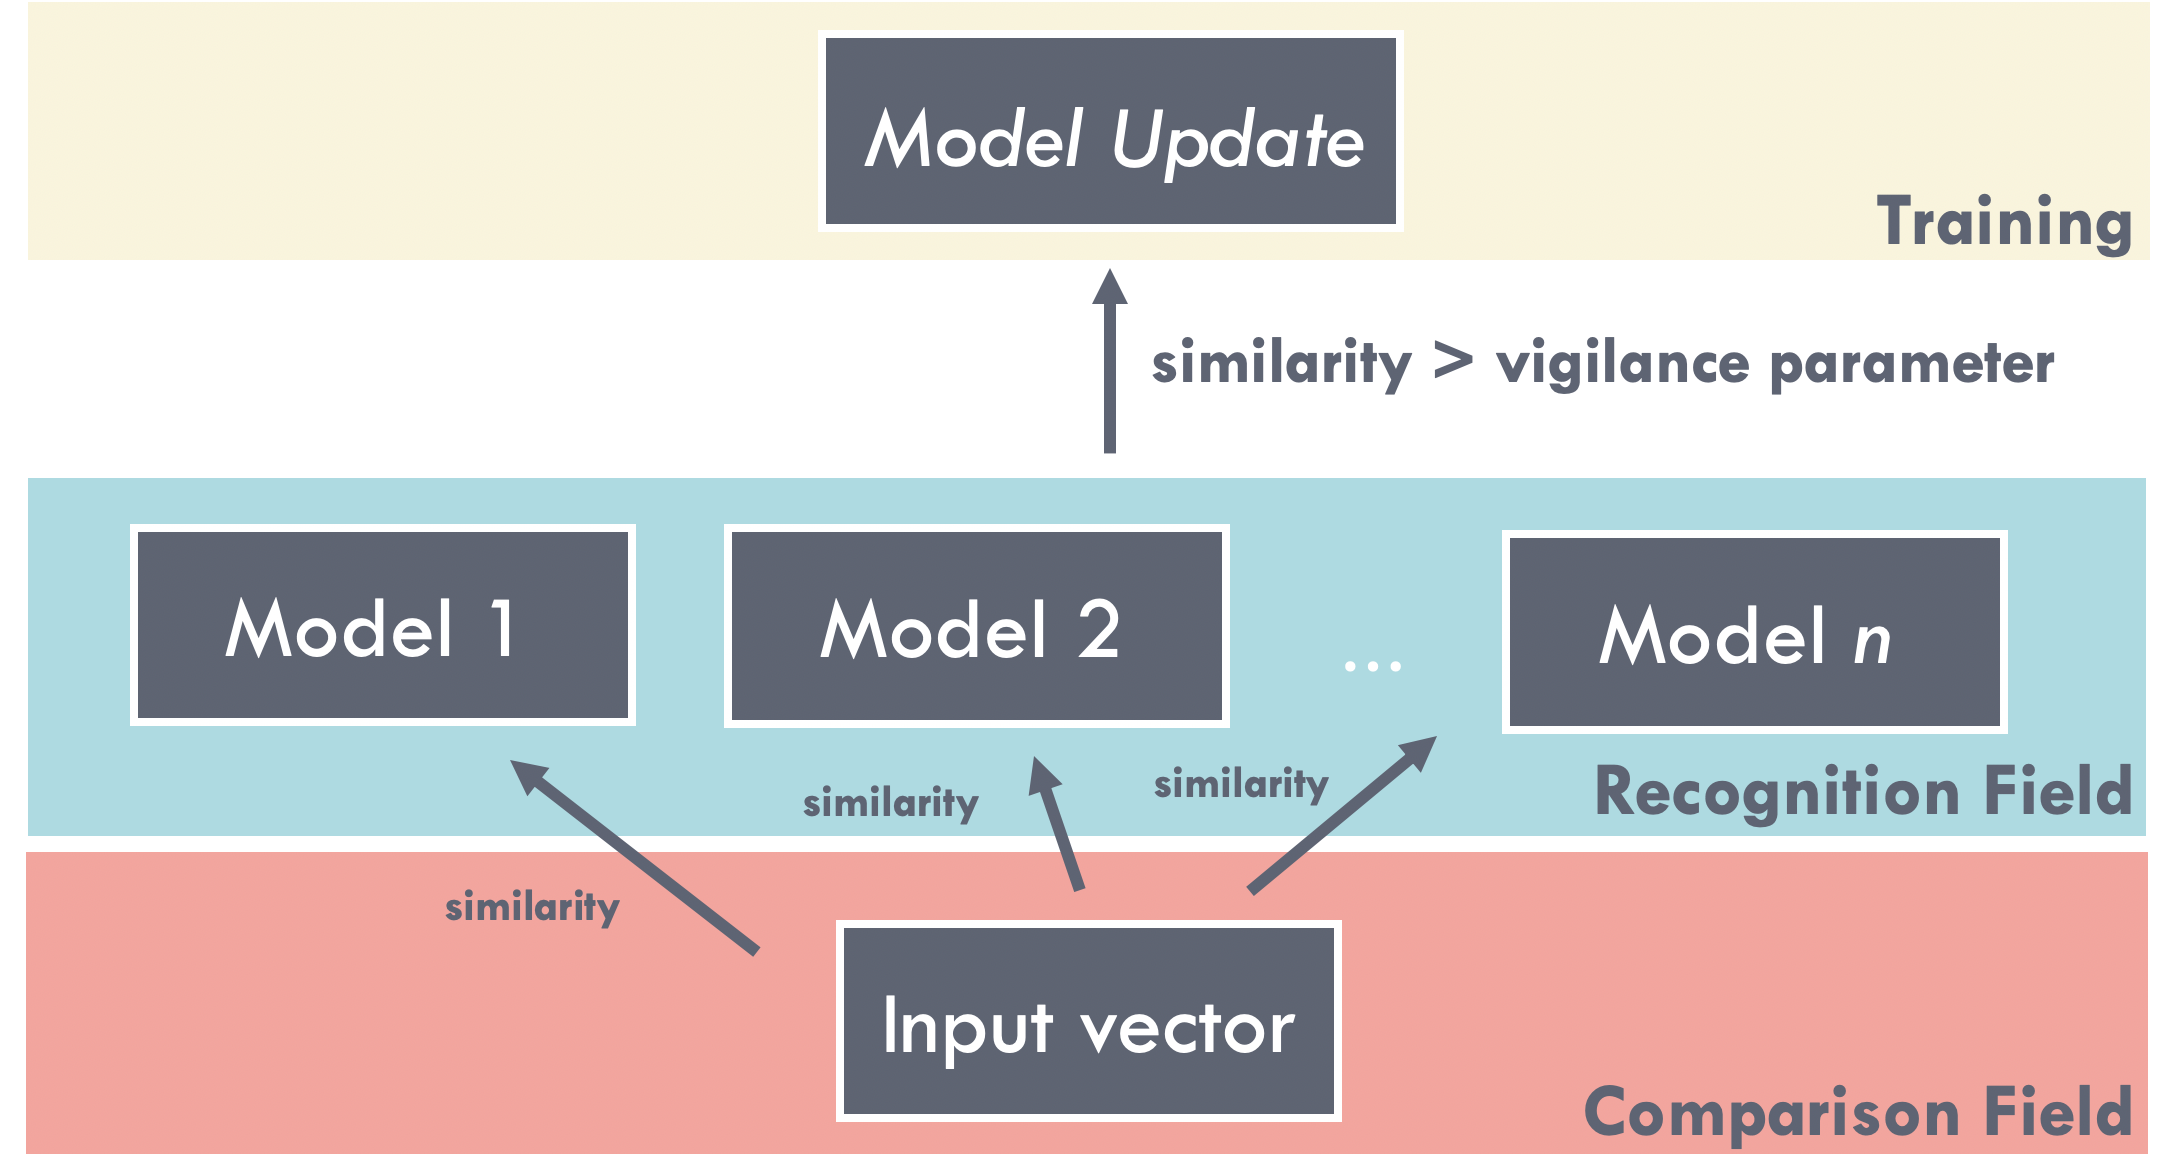
\includegraphics[width=\textwidth]{images/ch2/02art.jpeg}
    \caption{The simplified adaptive resonance theory architecture.}
    \label{fig:02art}
\end{figure}

Uniform sampling is a random sampling method where proportions of each desired group are forced to be sampled equally. For example, imagine a pump data set used to predict for the pump RPM given an input current.  The pump RPMs range between 0 - 1000 and the accuracy of the model is important across all values; however, the data set is significantly biased towards the 900 - 1000 RPM range, with only few data points in other regions. To ensure the model has acceptable performance across all values, the data set can be binned and equal amounts of data from each bin are sampled during the update step.  In the context of process control where data typically remain constant over long periods of time, uniform sampling can guarantee data variety during an incremental learning update step.

Lastly, experience replay is a method that gained popularity when it was first introduced to reinforcement learning to improve data efficiency and break temporal correlations \cite{dqn}. In experience replay, data (or experiences) are accumulated over time and are stored in a buffer.  During an update step, data is randomly sampled from the buffer to break temporal correlations that could potentially bias the models towards the most recent experience.  Additionally, data within the buffer can be re-used many times rather than being discarded after one update. Only after many time steps are the oldest memories removed from the buffer. An biological interpretation behind the algorithm is that humans create memories of past experiences.  Over the span of our lives, the same experiences are replayed many times; subconsciously when we eat, study, sleep, etc.  In doing so, humans can learn new experiences without catastrophically forgetting about past experiences; however, after an elongated period of time, distance unimpactful memories are forgotten.

By combining the advantages of the previous three topics, a new adaptive, outlier-robust, and data efficient algorithm catered towards the process control industry was developed.

\subsubsection{USIS Algorithm}

Figure \ref{fig:02USIS} shows the key steps for the USIS algorithm.  Initially, $n \geq 1$ models are present to model the system.  For input vectors in $n \geq 2$ systems, the distance $d$ between the input vector and the centroid of the data for each model is computed. This step is skipped for systems where $n = 1$ because only one $d$ is computed. The lowest $d$ is then compared to the neglect parameter, $\eta$ (opposite of vigilance parameter, $\nu$).  If $d \leq \eta$, the input vector will be added to the training archive (experience replay buffer) corresponding to the model.  Otherwise, the data point is transferred to the new model archive where data currently not belonging to any model is stored. In the new model archive, new models will be generated and added to the existing system of models after enough similar data is accumulated. Likewise, the training archives are used to incrementally update all models after a certain amount of data or time elapsed. During an update step, the archive data will be blended with additional uniformly sampled data from the historical archive (experience replay buffer) to avoid catastrophic interference. 

\begin{figure}
    \centering
    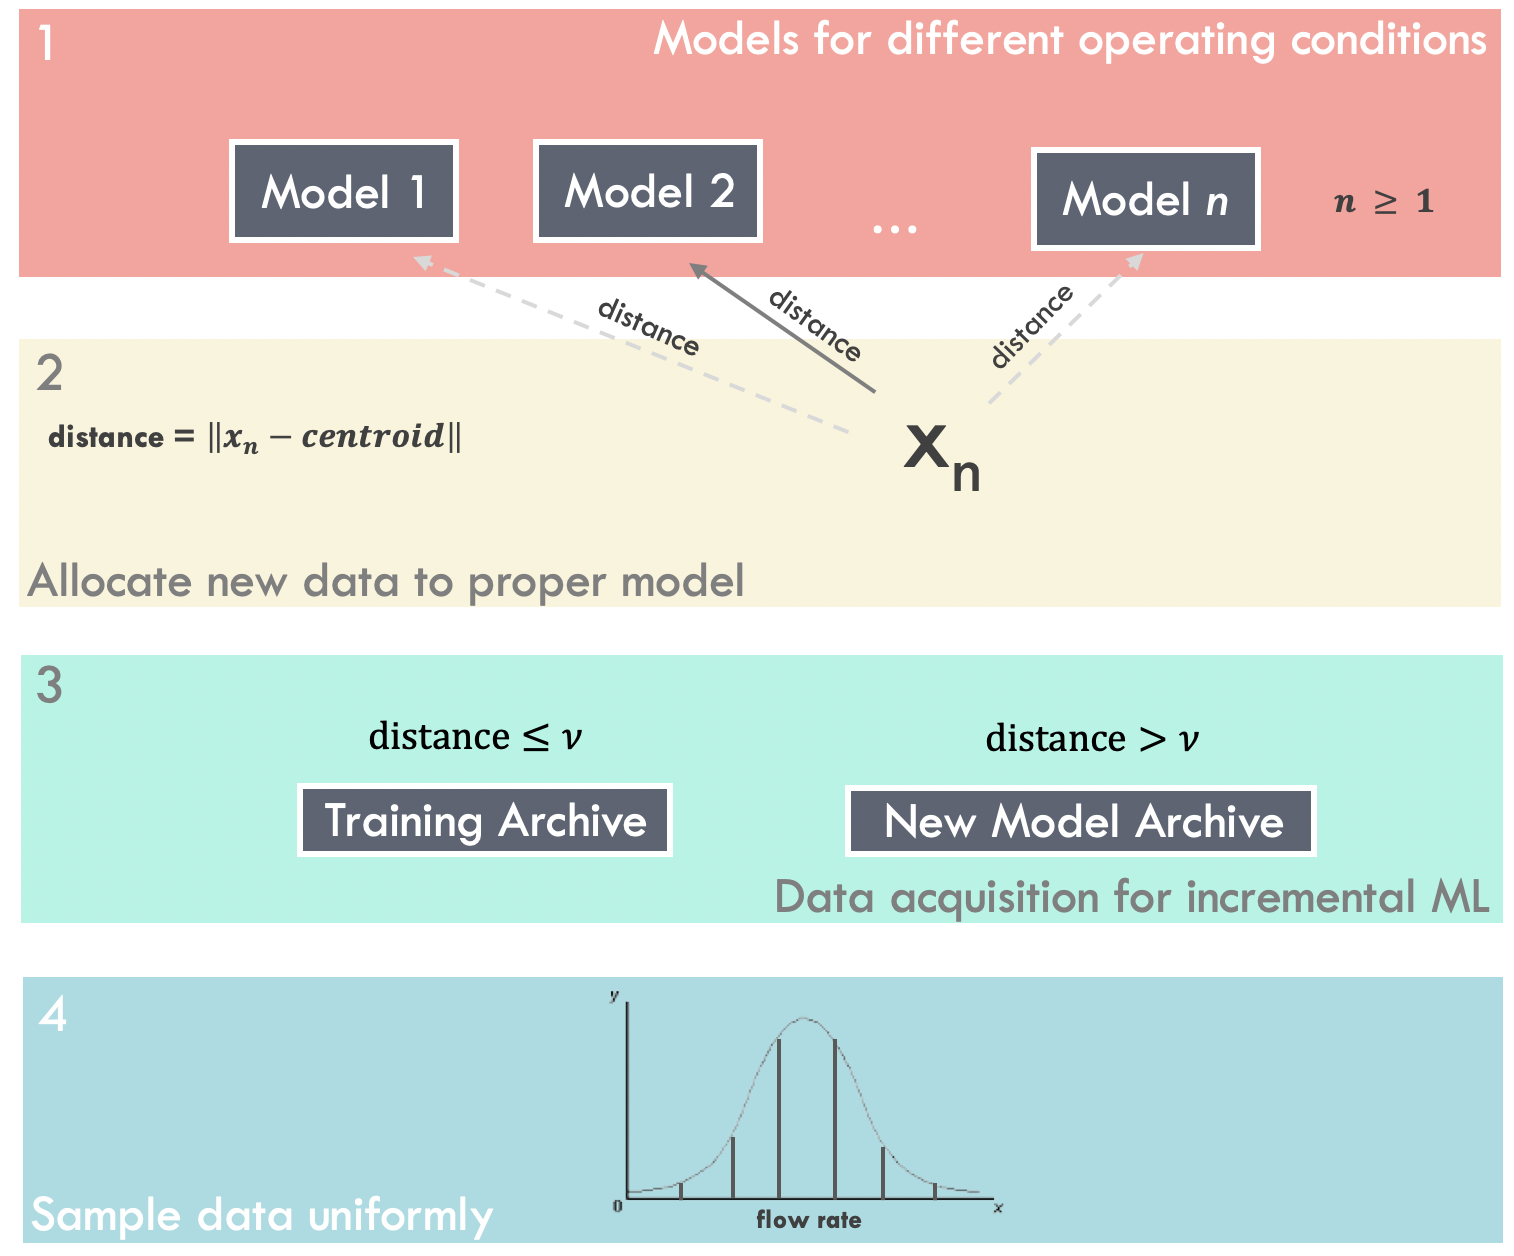
\includegraphics[width=\textwidth]{images/suncor/08IncrementalLearning.png}
    \caption{A brief visualization of the USIS algorithm.}
    \label{fig:02USIS}
\end{figure}

To enhance clarity of each update step, the data storage structure of USIS is shown in Figure \ref{fig:02USISData}. Before an update, the bins of each model must be defined.  The bins are typically defined by dividing the distribution of the predicted variable.  Bins can be narrower around regimes with abundant data, and wider for regimes lacking data.  During an update step, all data from the training archive alongside some sampled data from the historical training archive are blended together and fed into the gradient descent step for model updates.  Typically in process control applications, systems tend to linger around certain set points for many time steps.  Given this characteristic, the data in the training archives, consisting of $m$ training examples, typically belong to the same bin.  To avoid catastrophic interference when learning on elongated periods of similar operating conditions, $m$ examples of data from each bin in the historical archive is also sampled and assimilated with the training data when performing update steps. After the updates, all training archives are emptied by transferring the data into the historical archives.  When the historical archives get sufficiently full, the oldest data (or memories) are deleted.

\begin{figure}[h]
    \centering
    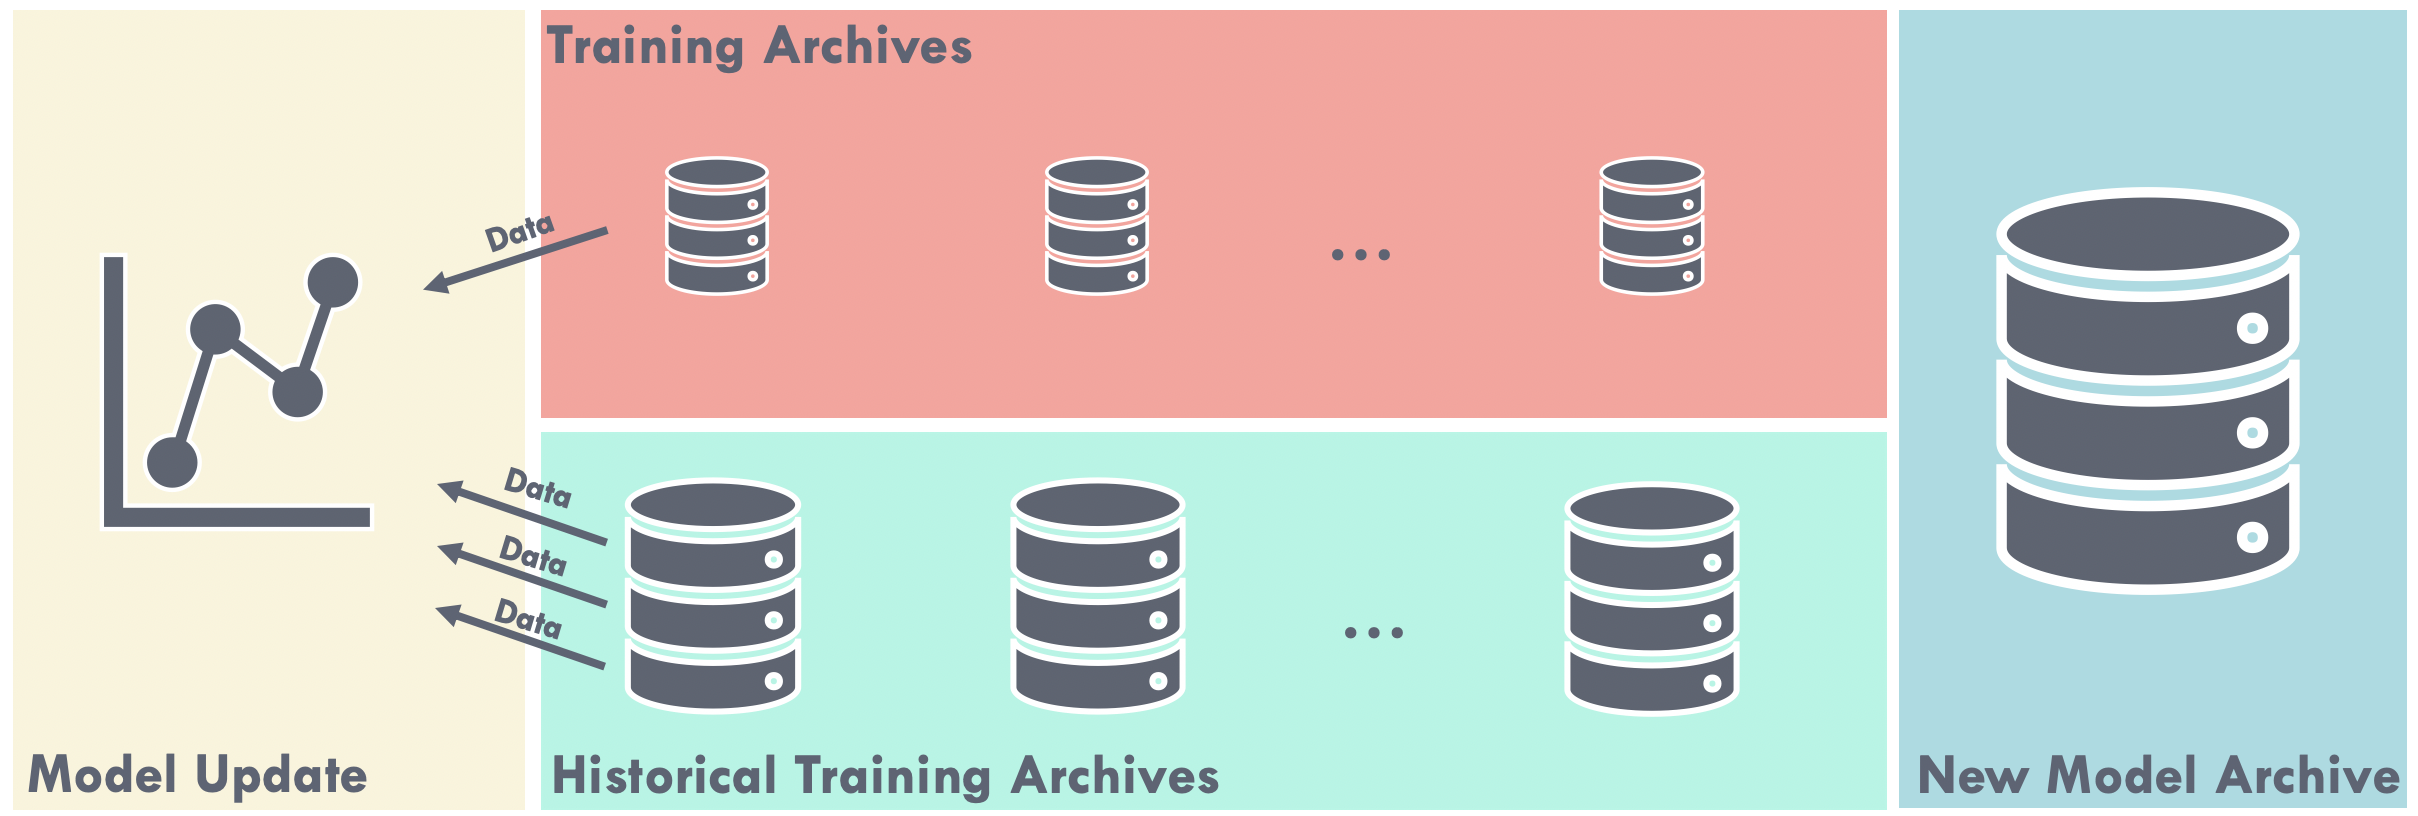
\includegraphics[width=\textwidth]{images/ch2/02USISData.jpeg}
    \caption{Data storage structure of USIS.}
    \label{fig:02USISData}
\end{figure}

The full USIS algorithm is shown in Figure \ref{fig:02USIS_Complete}.  There are five main tuning parameters of the USIS algorithm: i) when to update models; ii) bin size for each model; iii) neglect parameter; iv) distance metric; v) replay buffer size.

\begin{itemize}
    \item \textbf{i) Model Updates: } Common strategies for model updates are periodically, by example size, or when models exhibit large errors.  The first two are proactive methods, while the last is a reactive method.  In the periodically updating method, the models are automatically updated after a certain time has elapsed (e.g., update every 24 hours). Updates by example size refers to model updates after a certain amount of data is accumulated in the training archive. Only the model with adequate amounts of data is updated. For these two methods, there should not be a significant time gap between updates because updates may lead to excessive model changes otherwise.  Since this method is automated, significant model changes could potentially lead to sudden performance changes, jeopardizing production safety.  Model updating after large errors have incurred is the last method.  Here, the models are updated after an error threshold has been exceeded.  Compared to the previous methods where smooth update steps are performed, this method introduces significant changes to the model. Systems with highly noisy data and require inordinate amounts of manual data processing will benefit from this update style because completely automated updates may lead to model divergence.

    \item \textbf{ii) Bin size: } The bin size of each model should be tuned so the important sections  of the predicted variable can be properly predicted for each model. Additionally, the bin can be narrower for sections where abundant data is available and wider for sections where data is sparse.
    
    \item \textbf{iii) Neglect parameter: } Neglect determines the specialization of each model.  High neglect creates fewer generalized models, while low neglect produces many specialized models.  For highly non-linear multi-modal systems, low neglect may be the preferred choice; however, the initial setup and cost of ownership for such a system could potentially be high if automated updates are not implemented/feasible. On the other hand, high neglect systems are cheaper to maintain due to the reduced number of models, but the accuracy may suffer.  Picking a proper neglect parameter represents the trade-off between accuracy and complexity.  A general rule of thumb for the neglect parameter would be the radius of the cluster.  For example, $\eta$ for a cluster identified using DBSCAN would be its $\epsilon$ value.
    
    \item \textbf{iv) Distance metric: } The Euclidean distance between the input vector and the historical data is the recommended choice; however, other distance metrics can be used for specialized applications.
    
    
    \item \textbf{v) Replay buffer size: } The replay buffer size can also be tuned to adjust when old memories are no longer relevant (intuitively, forgetting older memories).  For processes where operating conditions are changing frequently, it would be beneficial to have smaller replay buffers to avoid learning on obsolete data.  Replay buffers can also have an adaptive size depending on the current prediction error as proposed in \cite{eff_of_er}; however, such a method is still embryonic and further exploration should be conducted before implementation.
\end{itemize}

\begin{figure}[h]
    \centering
    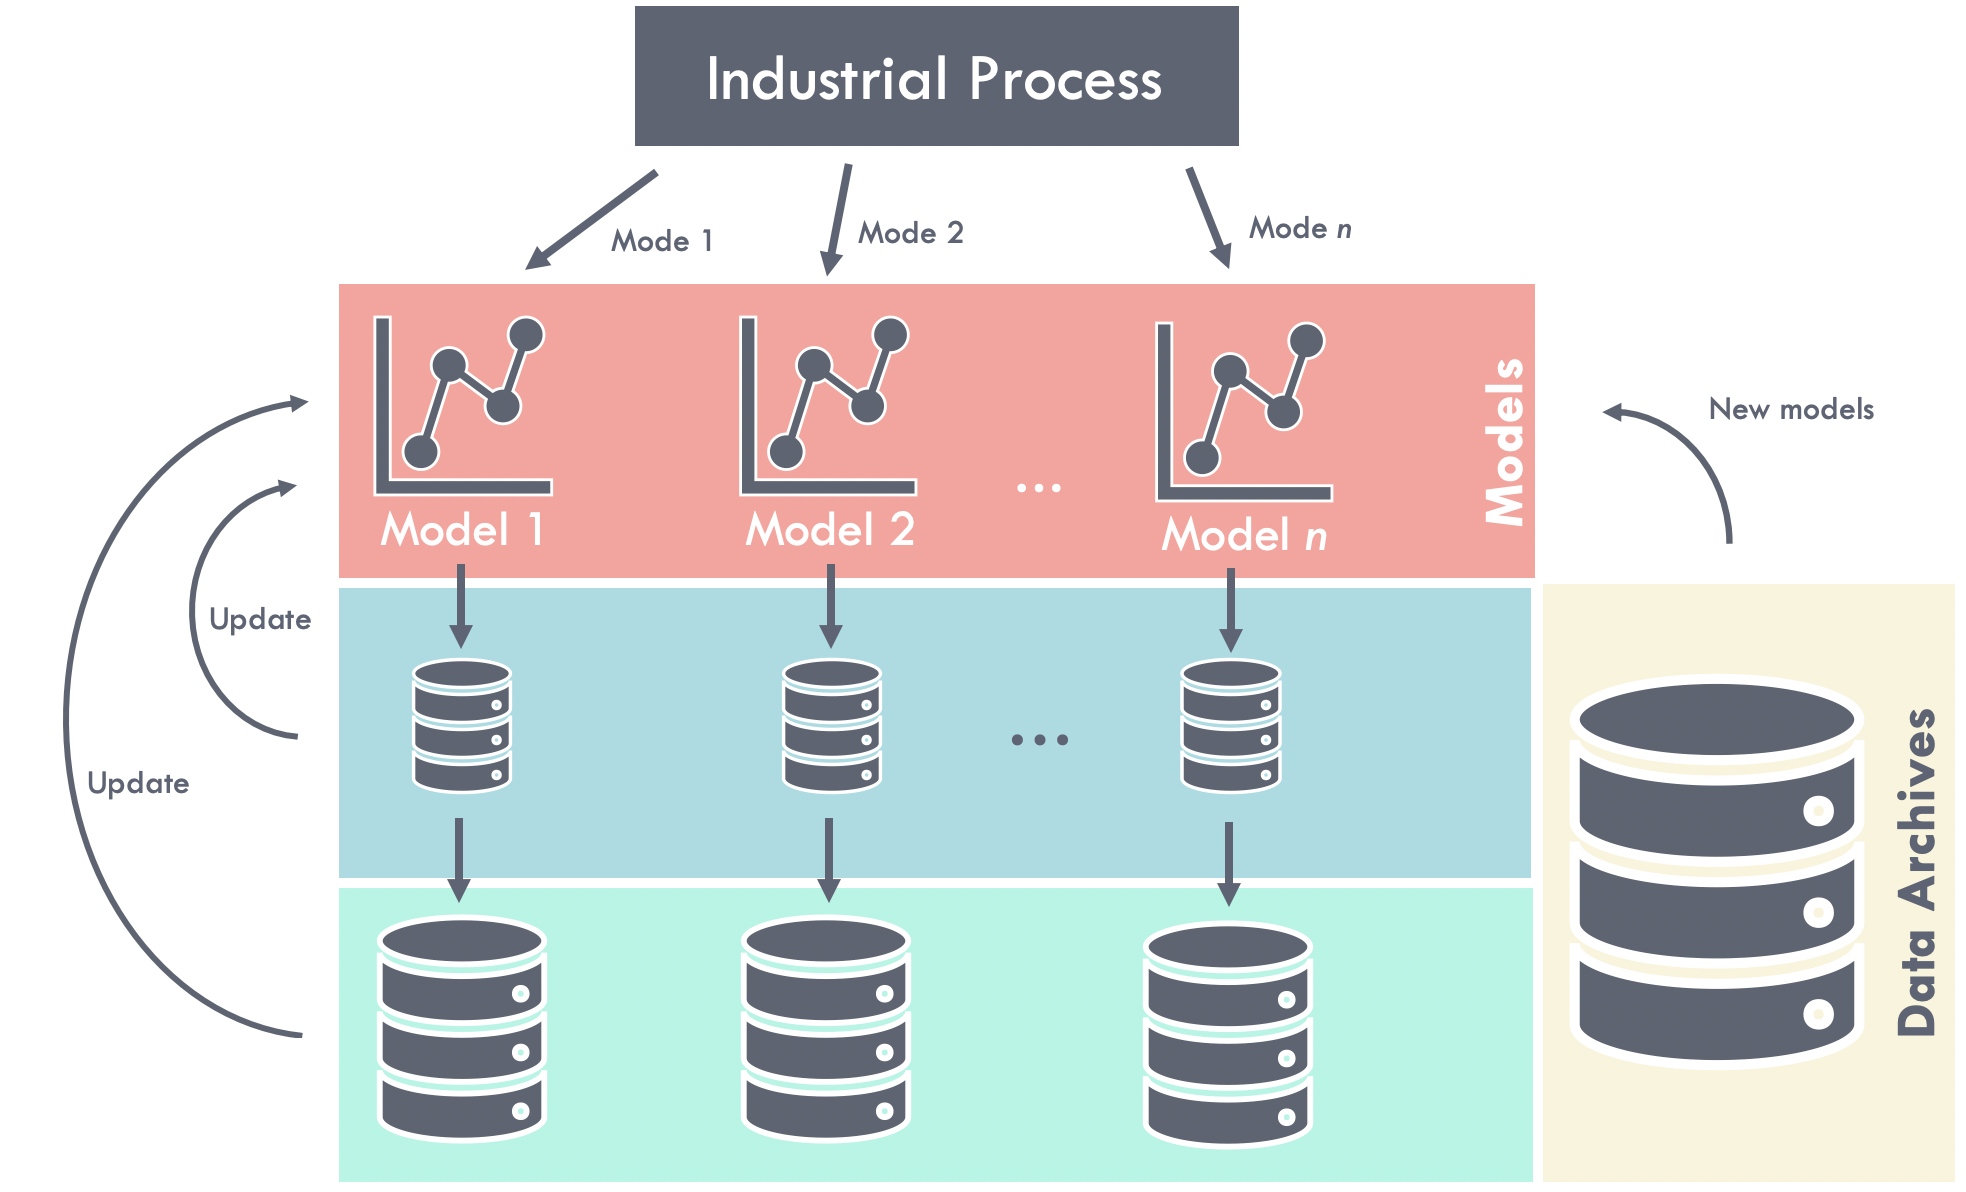
\includegraphics[width=\textwidth]{images/ch2/02USIS_Complete.jpeg}
    \caption{The complete USIS architecture.}
    \label{fig:02USIS_Complete}
\end{figure}

Uniform sampling in USIS can also be swapped out for importance sampling, where high error examples are prioritized for the next sampling cycle (motivation from \cite{prioritize_exp_replay}. In doing so, high error examples (biologically modelled as 'shocking' experiences) have higher probabilities of being recalled.  Intuitively, humans recall 'shocking' experiences more often. The method enhances accuracy in many reinforcement learning applications \cite{dqn, er1, er2}, although, such a method may prioritize noisy, near-outlier data points in process control applications and introduce model divergence.

\section{Discussion: Cheaper, More Accurate, and Adaptive?}

Machine learning has promised cheaper, more accurate, and adaptive solutions for industries around the world.  However, applying ML solutions naively into the process control industry yields no significant value due to various unique factors in process control data.  So far in this chapter, different data pre-processing methods catered towards the process industry were introduced.  General ML methods and their applicability were correlated to the process control industry. By innovatively combining parts of separate algorithms, a new algorithm catered towards the process industry, USIS, was also introduced. USIS is an adaptive, outlier-free, model structure that can be used to model a process with many operating conditions while avoiding catastrophic interference. But are these solutions truly cheaper, more accurate, and adaptive? 

The comparison between ML prediction solutions and traditional methods is shown below for common areas where ML is implemented today:

\begin{itemize}
    \item \textbf{Cheaper: } ML soft sensors will definitely be cheaper for difficult-to-measure process variables where lab test must be conducted.  Conducting lab measurements may cost up to hundreds of thousands per year if frequent measurements are required.  Initial cost for soft sensors may be high because a ML expert must collaborate with process operators to first develop the soft sensor(s); however, on-going costs for this application is minuscule.  Soft sensors for prediction of variables that are difficult to measure are definitely cheaper than buying a highly advanced physical sensor.  Lastly, prediction applications used for operator training or forecasting should be significantly cheaper compared to having a senior operator on shift explicitly to train a new operator or hiring a group of subject matter experts to forecast future production possibilities.
    \item \textbf{More Accurate: } Soft sensors used to predict lab measurements could yield high accuracy, but will never exceed lab measurements.  This is because lab data is used to train the soft sensor; hence, serving as a performance ceiling.  For soft sensors used to predict for difficult to measure process variables, the accuracy will depend on the quality of the data used to build the soft sensor.  Additionally, the accuracy vary from application to application.  For predicting for heights in a primary separation vessel using cameras and the sight glass, the accuracy can be extremely high.  On the other hand, predicting the density of a crude given highly noisy readings and poor input data may be nearly impossible.
    \item \textbf{Adaptive: } The adaptability factor of ML algorithms is purely dependent on available feedback.  For applications where immediate feedback is available, such as predicting for a continuously measured output variable, adaptability is trivial.  However, ML solutions cannot adapt for tasks where no feedback exists.  One example of a non-adaptive ML application would be soft sensors for prediction of lab measured process variables. If no additional lab measurements are taken after the soft sensor is live, it will never adapt.  Therefore, it is good practice to continue obtaining lab measurements seldomly to evaluate the soft sensor performance. For tasks requiring adaptation, ML solutions should be the preferred choice because human operators would have a hard time remembering all the historical data.
\end{itemize}

To summarize, ML prediction applications are generally cheaper compared to their traditional counterparts.  This is simply because applications that requires ML are typically expensive and are solved poorly using traditional approaches to begin with.  In terms of accuracy, ML solutions would not exceed the performance of a lab tested process variable; however, may surpass accuracy given representative data sets or unique applications.  Lastly, ML solutions can only adapt if proper feedback is available for the algorithm. 

\section{Highlights of ML Application onto a Pipeline}

The methods and algorithms in this chapter were applied onto an industrial pipeline\footnote{Many values are significantly rounded and/or omitted to maintain confidentiality of the project}\footnote{The algorithms are live as of May $7^{th}$, 2019 on one industrial pipeline. Work is being done to clone the project onto a second line.}.  The highlights of the implementation will be shown in this section.  For a detailed project report, please refer to Appendix A.

\subsection{Process Description}
Pipelines are critical assets for the transport of fluids safely and efficiently across long distances. Fluids include petroleum products, clean water, natural gas, sewage, and even beer. In Canada, over 97\% of petroleum products are shipped by pipeline alone.  Due to the mission critical nature of pipelines on society's success, ensuring its reliability and efficiency has global-scale impact.  Typical pipelines may contain hundreds of digital sensors littered across the pipeline.  Such information overload may be overwhelming for humans; however, ML methods benefit greatly from the abundance of data.  Here, an opportunity was discovered where ML methods can be applied to greatly increase the robustness and efficiency of the pipeline.  For phase one of the project, ML prediction models were built to create a digital twin of the pipeline for operator training programs and future optimization purposes.

A schematic of the pipeline is shown in Figure \ref{fig:02RM06A}.  The highly complex pipeline spans over 100 kms and carries two products, a lighter product and a heavier product. The two products are batched (i.e., rotate between sending each product) and each product is sent for approximately eight hours before switching to the other product. The American Petroleum Institute (API) gravity for the lighter and heavier products are roughly 40 and 20, respectively. For the rest of this chapter, the lighter and heavier product will be referred to as \textit{light crude} and \textit{heavy crude}, respectively. The pipeline is typically operated between 1800 bbl/h to 3050 bbl/h. 

\begin{figure}[h]
    \centering
    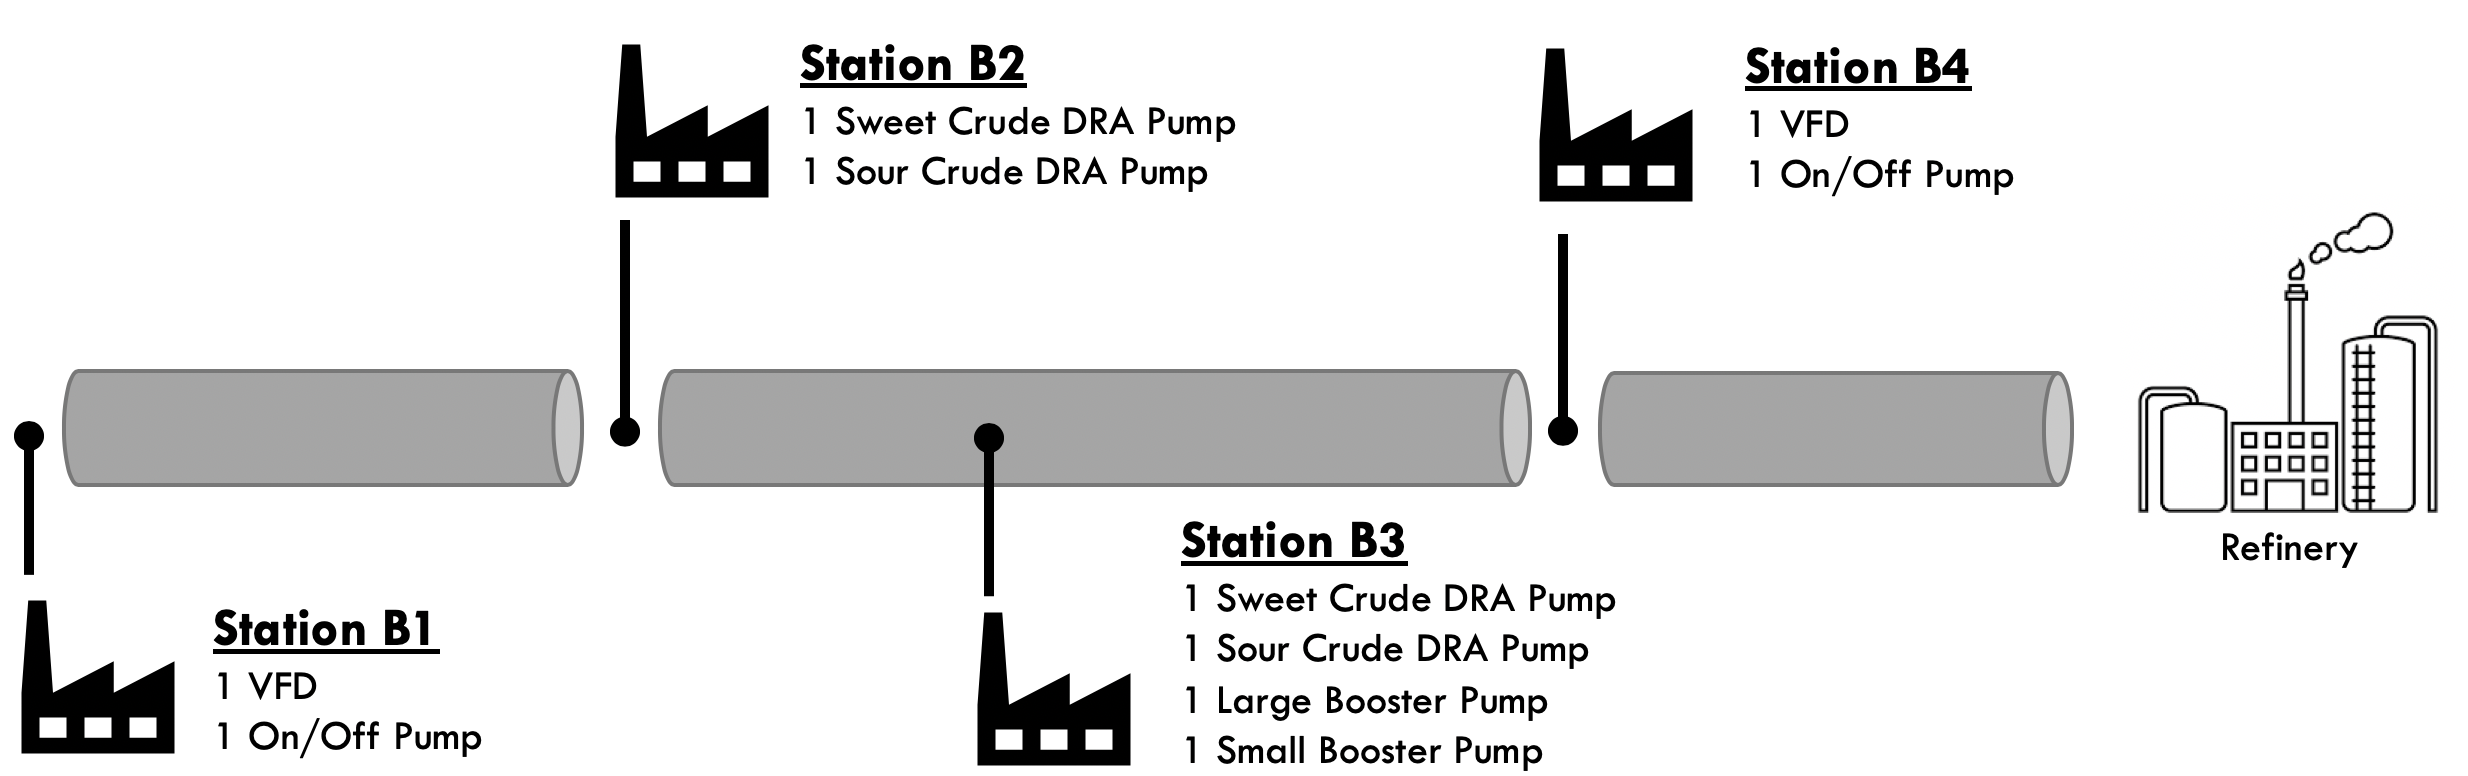
\includegraphics[scale=0.33]{images/suncor/08RM06A.png}
    \caption{Schematic diagram of Line B.}
    \label{fig:02RM06A}
\end{figure}

Equipment wise, Line B boasts eight pumps spread across four pump stations. Two pumps are variable frequency drives (VFD), while the rest are on/off pumps. Additionally, there are four drag reducing agent (DRA) injection pumps situated at the second and third pump stations. Each pump station contains a heavy crude and light crude DRA pump because the different crudes use different types of DRA.  The DRA is injected based on the product present at the pump station. 

\subsection{Data Pre-processing}
The industry sponsors initially provided a data set containing 899 tags and 525,601 data points for each tag.  The data pre-processing step was deconstructed into three phases for this project: pre-processing by subject matter experts, automated data pre-processing, and manual data pre-processing. The first two phases are typical of any machine learning project.  The third phase contains methods introduced in this chapter. Upon completion, an on-going iterative data pre-processing procedure continued until the end of the project to ensure industrial sponsors were satisfied with the model performance. The objective of the prediction models were to predict the \textbf{output flow rate} as a function of process variables.

The data was first pre-processed by experts within the sponsor's organization to remove useless tags such as alarm limits, fire detector status, and the sort.  After doing so, the amount of tags was reduced to 124.  The remaining data was sent into various automated data pre-processing algorithms to further remove redundant/insignificant tags.  The algorithms include: missing data removal, data imbalance analysis, and collinear analysis.  Missing data removal cleans up any NaN or empty values in the data set.  Data imbalance analysis inspects all categorical variables and removes heavily imbalanced tags where one class significantly dominates all other classes.  Lastly, collinear analysis identify heavily correlated columns and removes all but one to prevent redundancy in the data set. Total tags reduced to 65 after the automated feature selection.

Next, the manual pre-processing was conducted on the data set.  First, engineering knowledge was applied to the pre-processing step to remove segments of data where the process exhibits abnormal operating behaviour.  Then, the data at each pump station was shifted to incorporate time delays. In pipelines transporting incompressible fluids, pressure propagates down at the speed of sound (1480 km/h) \cite{fluid_mechanics}; therefore, all pressure variables were shifted with accordance to their distance to the output of the pipeline (shown in Table \ref{tab:02TimeToCC}.  Likewise, DRA also had time delay.  DRA must be transported down the entire pipeline to exhibit its full drag reducing effect.  From giving flow rates and the length of each segment of the pipeline, it was calculated that coating the entire pipeline required approximately ten hours.  Therefore, the first ten hours data corresponding to a set point change in DRA was removed to ensure the DRA's effect has been fully realized in the output flow rate data.

\begin{table}[h]
    \centering
    {\setstretch{1.2}
    \begin{tabular}{ p{6cm} | c | c | c | c}
             & B1 & B2 & B3 & B4 \\
        \hline
        Time to refinery at speed of sound in liquids (1480 m/s) \cite{fluid_mechanics}
        &  2.0 min  &  2.0 min  &  1.0 min  &  1.0 min  \\
    \end{tabular}}
    \caption{Time required for pressure changes at each pump station to be realized at refinery.}
    \label{tab:02TimeToCC}
\end{table}

Additionally, the temperature and DRA ppm measurements were highly noisy and were exponentially smoothed using Equations \ref{eq:08EWMA} to increase reliability.  The pre- and post-smoothed values of the DRA are shown in Figure \ref{fig:02DRA} to illustrate the effect of exponentially smoothing.

\begin{figure}
     \centering
     \begin{subfigure}[b]{0.9\textwidth}
         \centering
         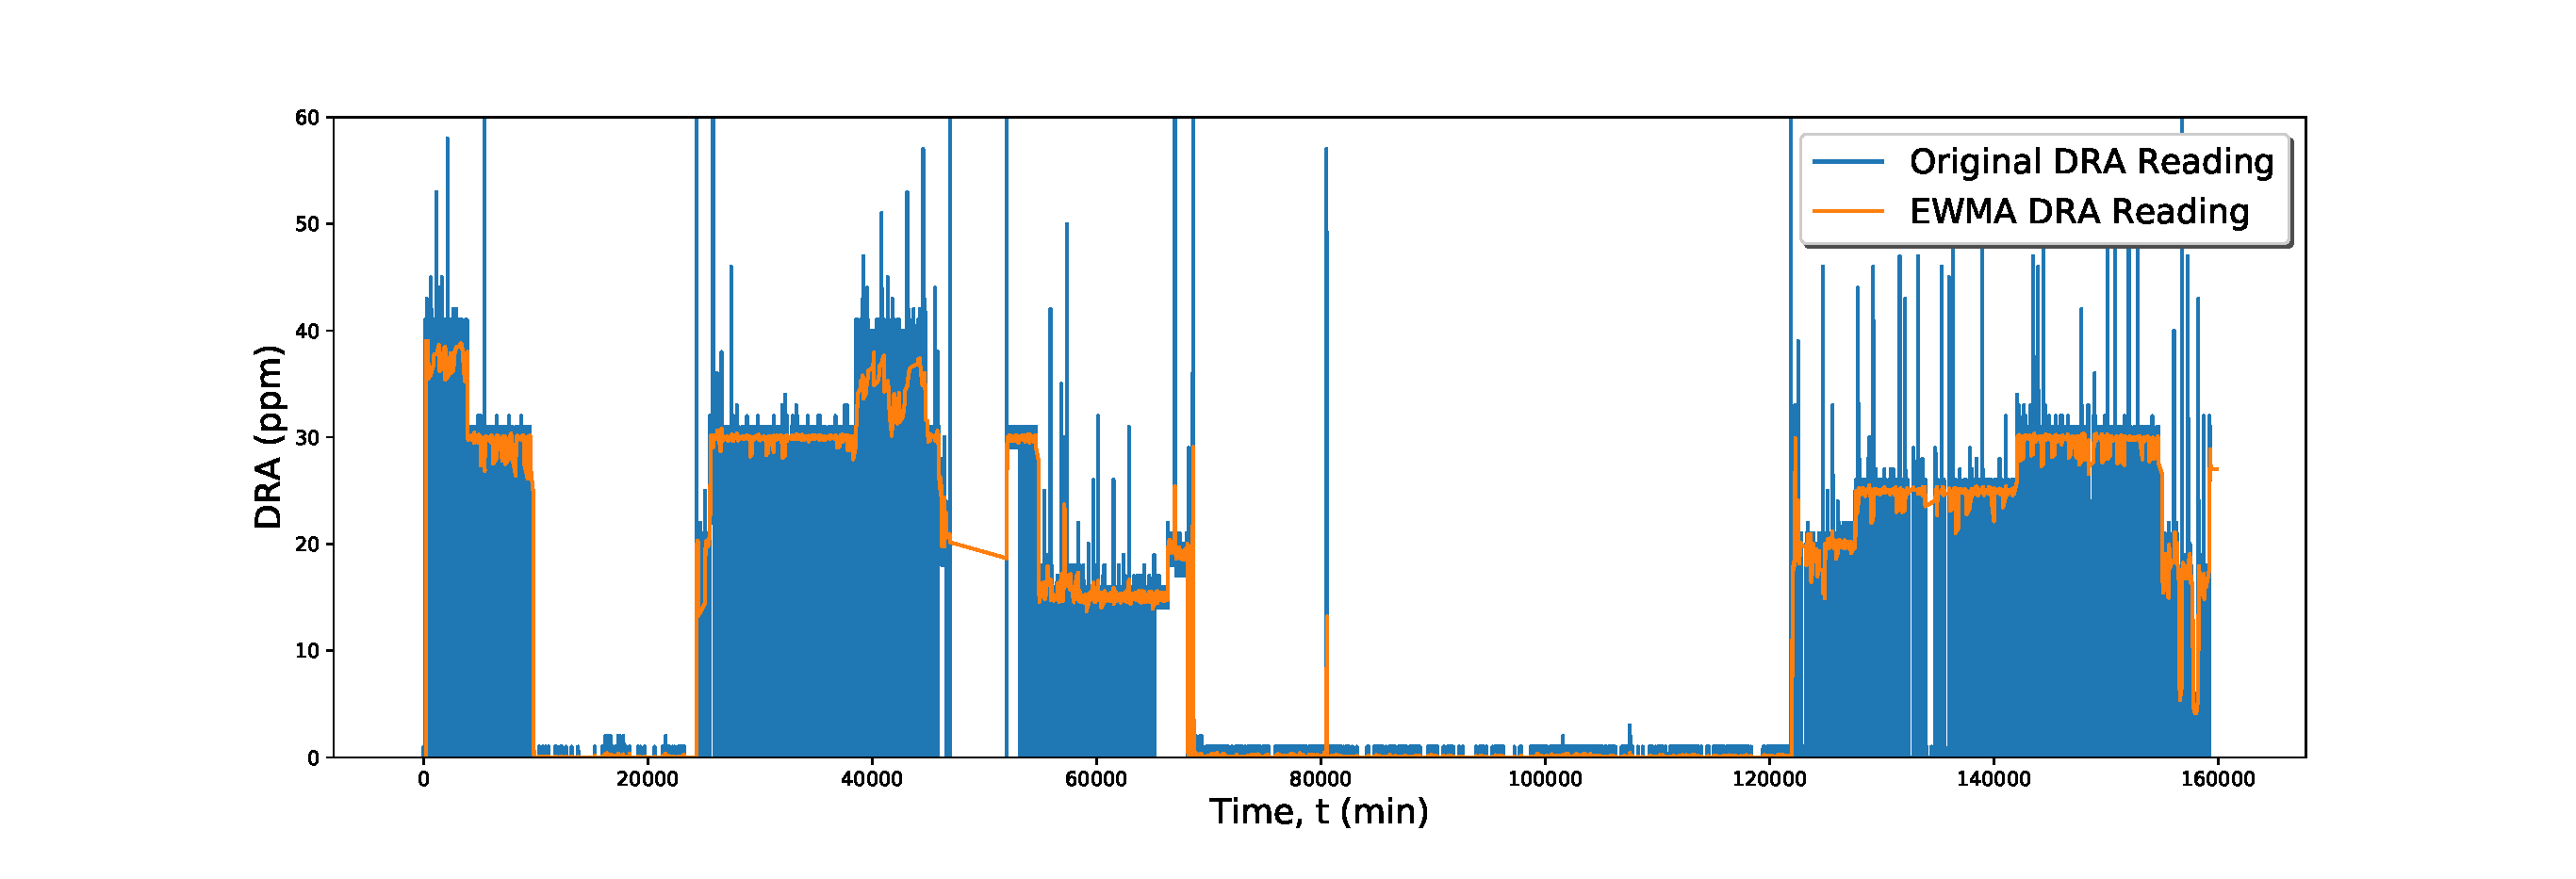
\includegraphics[width=\textwidth]{images/suncor/08CIGSour.eps}
         \caption{Station B2 heavy DRA sensor reading.}
     \end{subfigure}
     \begin{subfigure}[b]{0.9\textwidth}
         \centering
         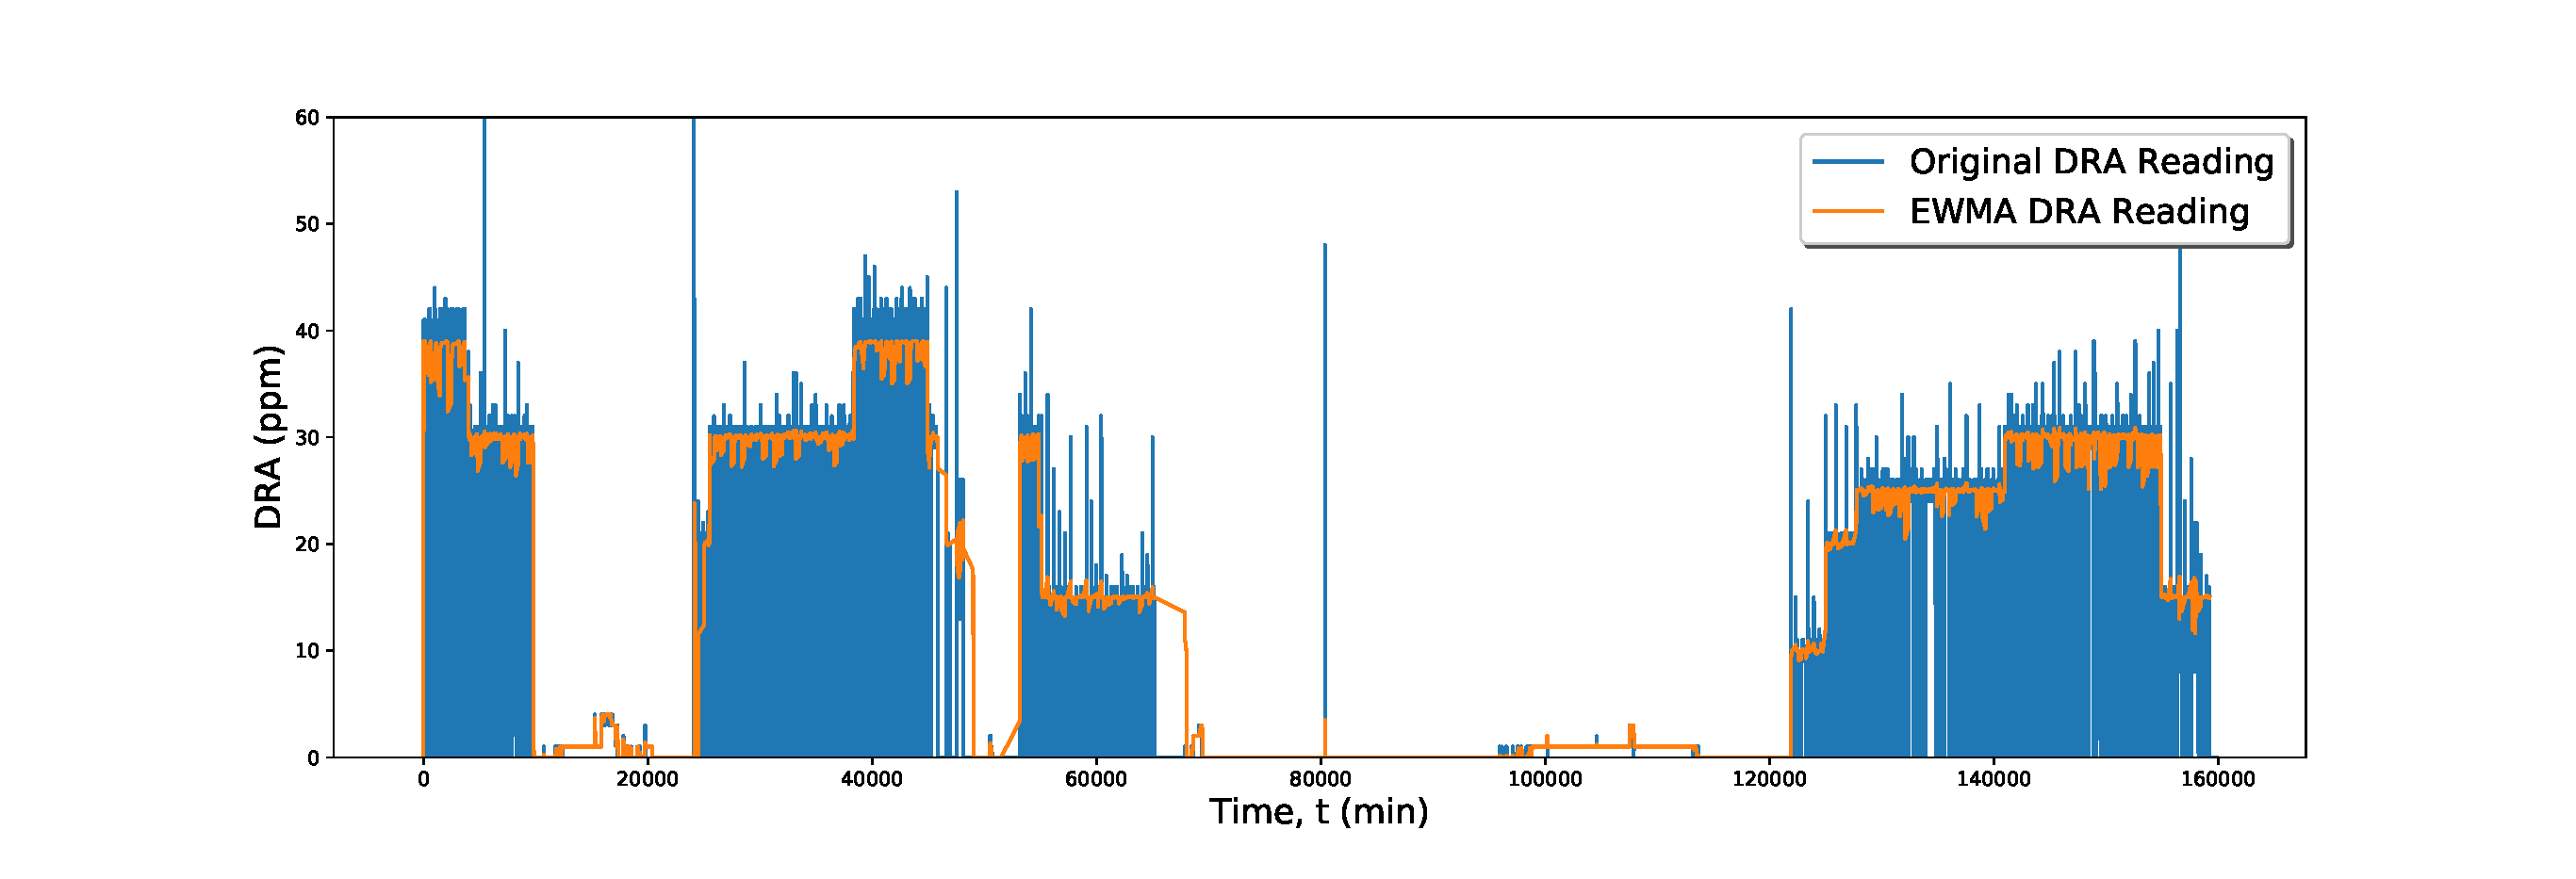
\includegraphics[width=\textwidth]{images/suncor/08CIGSweet.eps}
         \caption{Station B2 light DRA sensor reading.}
     \end{subfigure}
     \begin{subfigure}[b]{0.9\textwidth}
         \centering
         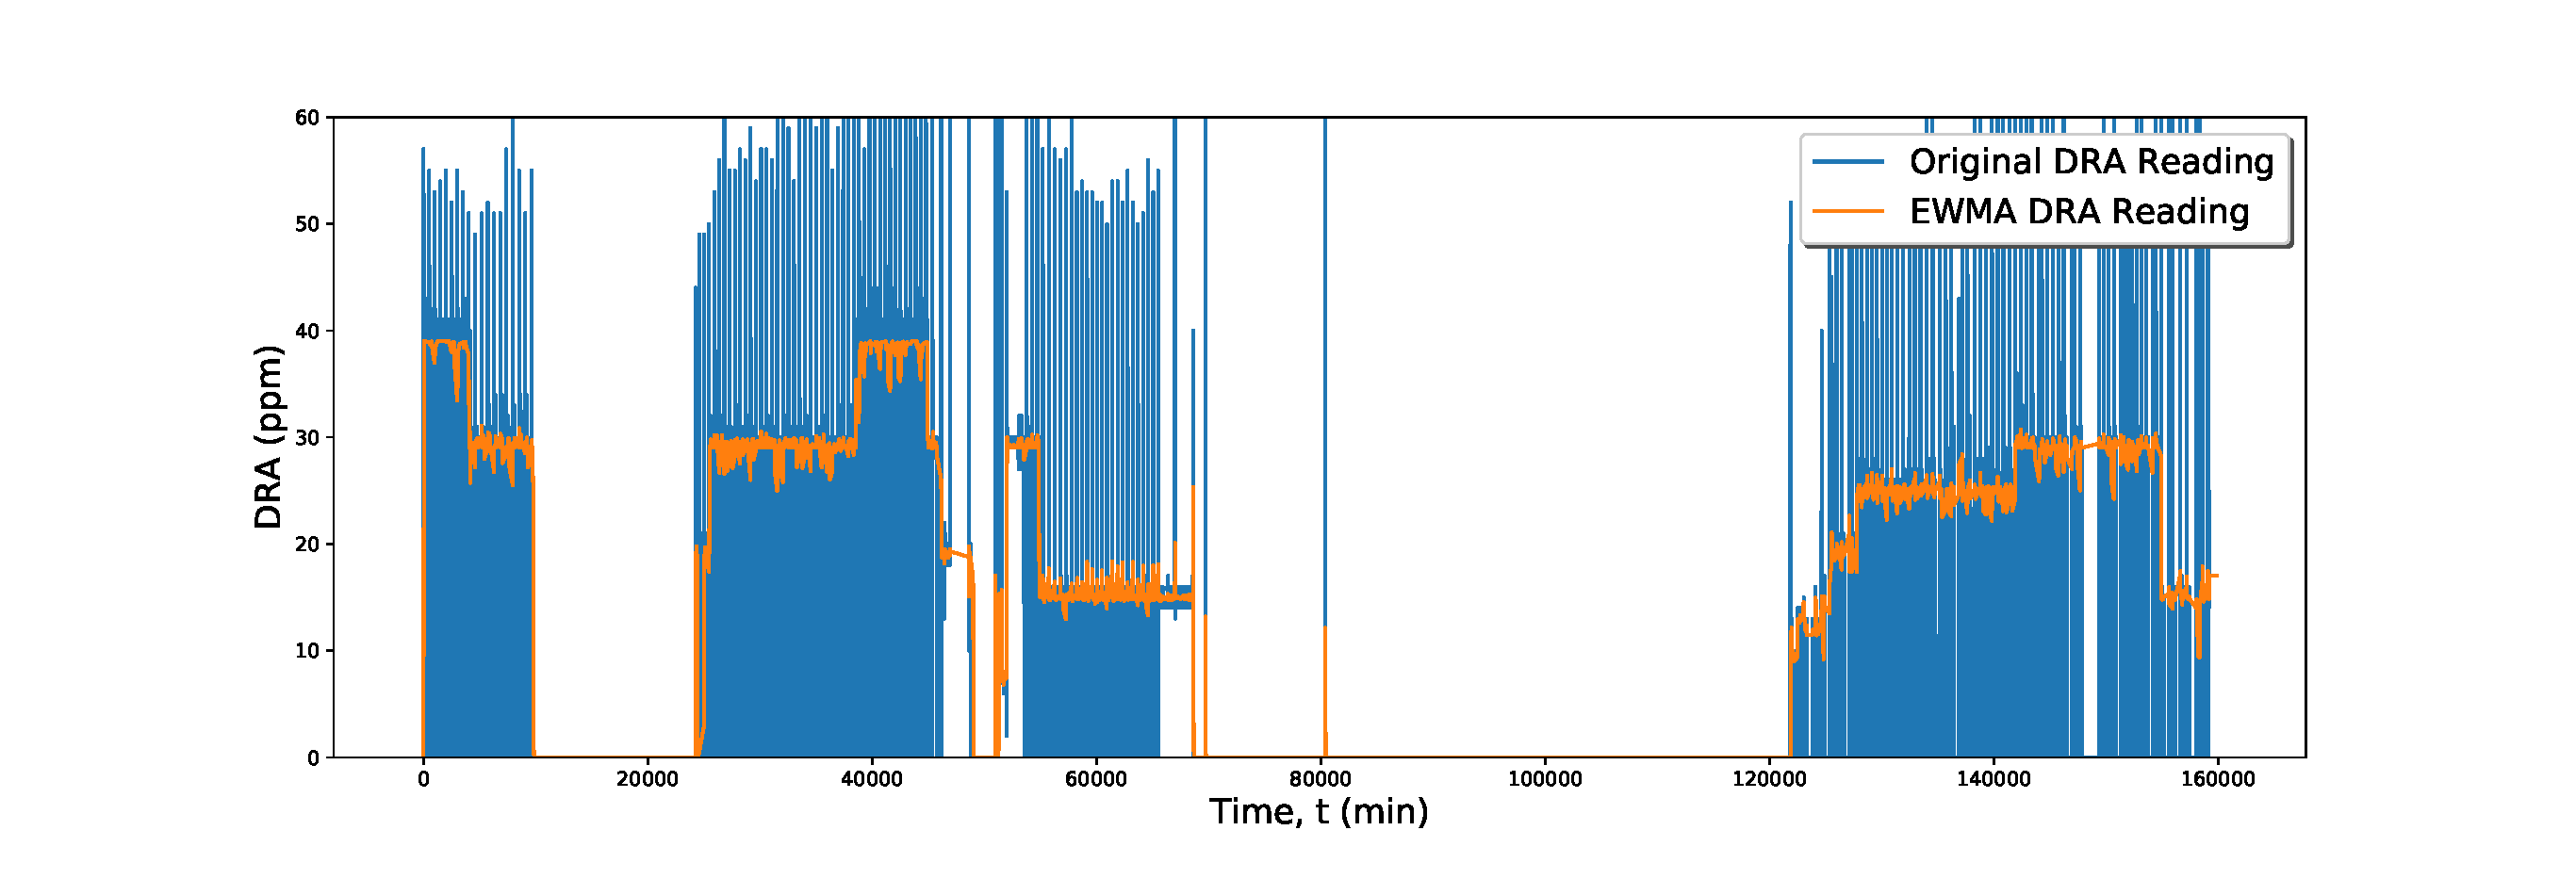
\includegraphics[width=\textwidth]{images/suncor/08AultSour.eps}
         \caption{Station B3 heavy DRA sensor reading.}
     \end{subfigure}
     \begin{subfigure}[b]{0.9\textwidth}
         \centering
         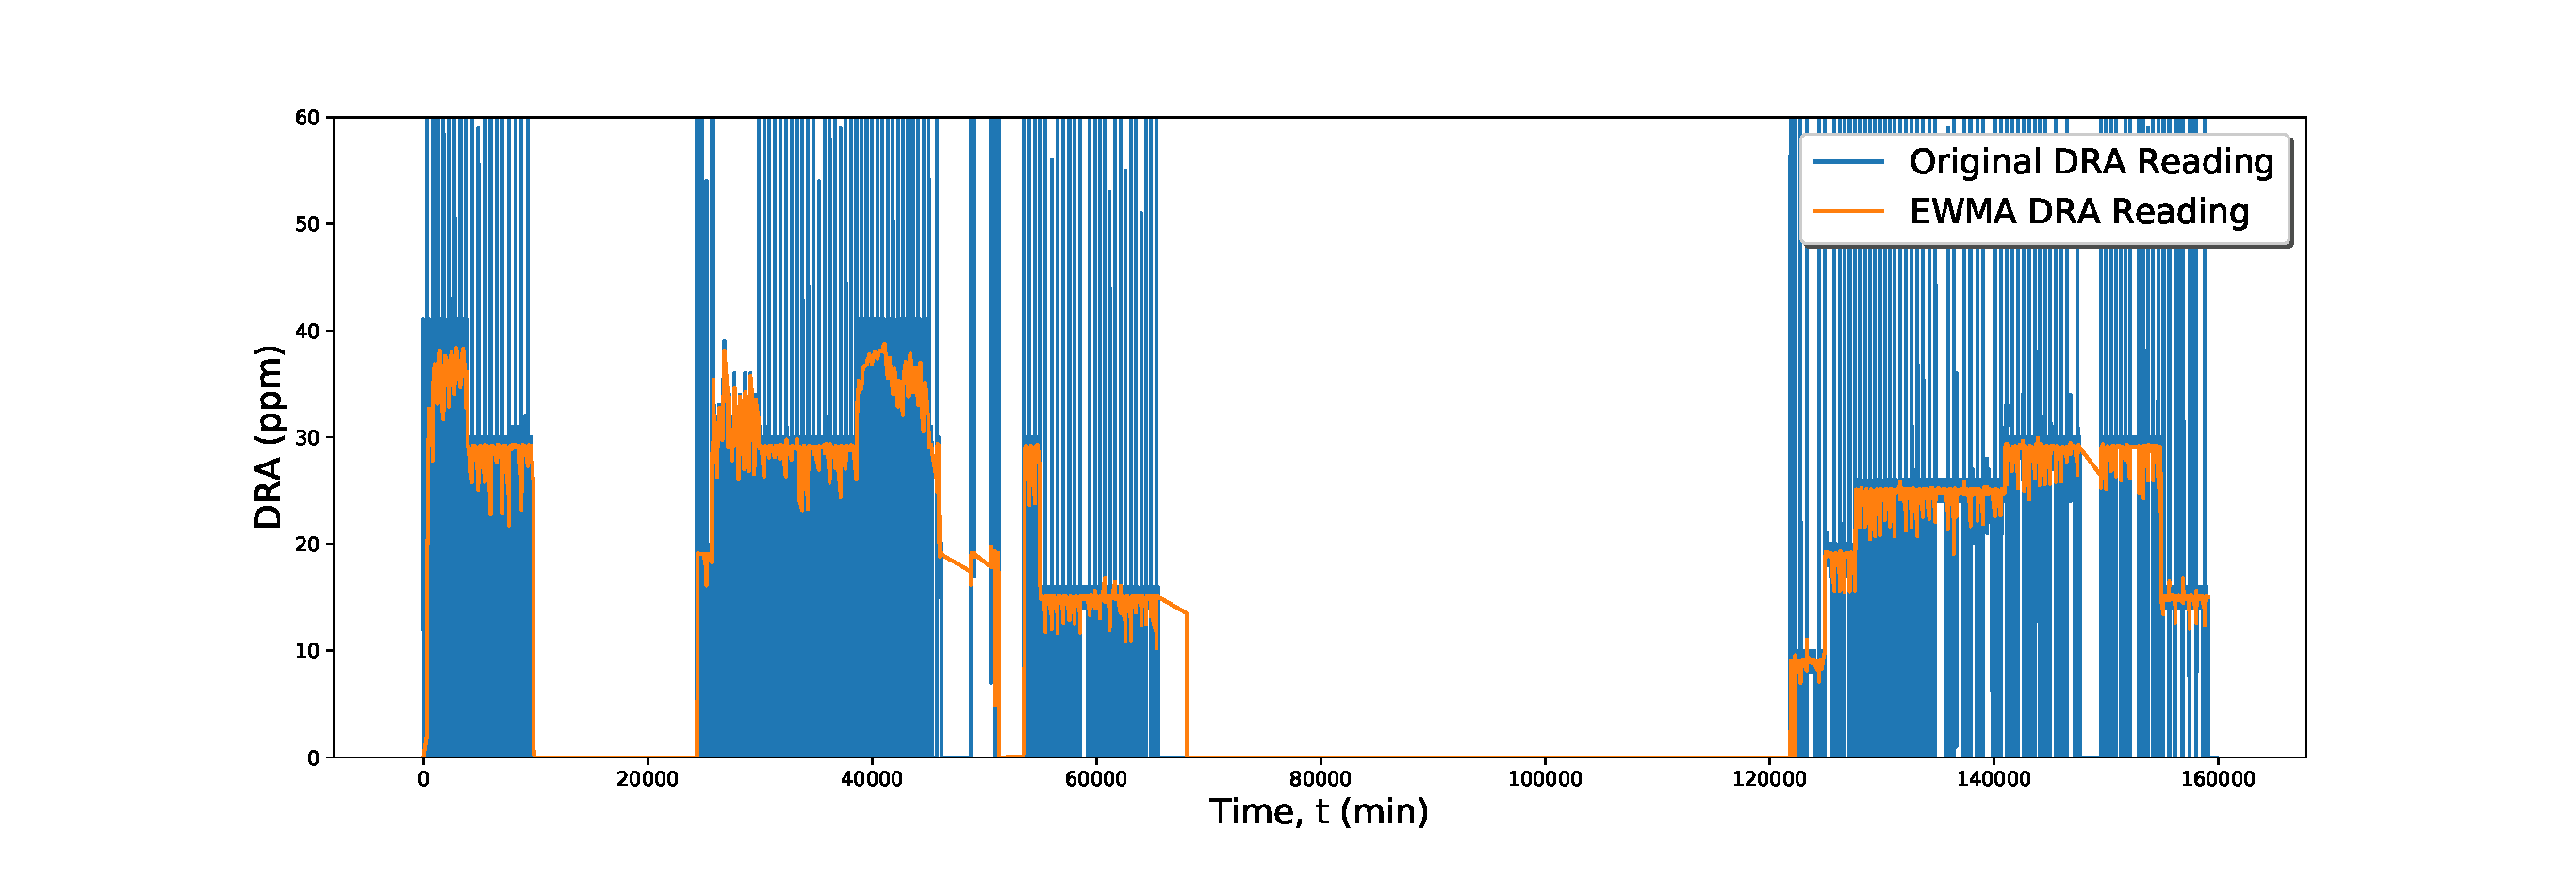
\includegraphics[width=\textwidth]{images/suncor/08AultSweet.eps}
         \caption{Station B2 light DRA sensor reading.}
     \end{subfigure}
        \caption{Pre- and post-processed DRA sensor readings.}
        \label{fig:02DRA}
\end{figure}

To conclude the data pre-processing procedure, the process operators were consulted with to identify any "special" considerations that should be included into the ML models.  Here, the operators stated that the density reading is unreliable and is only used to identify the crude type at each station. From this information, all density readings were feature engineered into binary readings where "1" represented light crude and "0" represented heavy crude to reflect the physical purpose of the reading.

Exploratory data analysis was then performed on the processed data to gain additional insight. In Figure \ref{fig:02KDE}, a kernel density estimation was applied to the pipeline outlet flow rate to identify its distribution as shown.  It can be seen that the flow rate follows a bi-modal distribution and most likely corresponds to two different operating regimes. To enhance ML model performance, the two modes were segregated using DBSCAN.  Here, DBSCAN was selected due to its scalability to big data and ability to identify outliers. The hyper parameters, $\epsilon$ and $min \; points$, for DBSCAN were 1.13 and 10,000, respectively.

\begin{figure}[h]
    \centering
    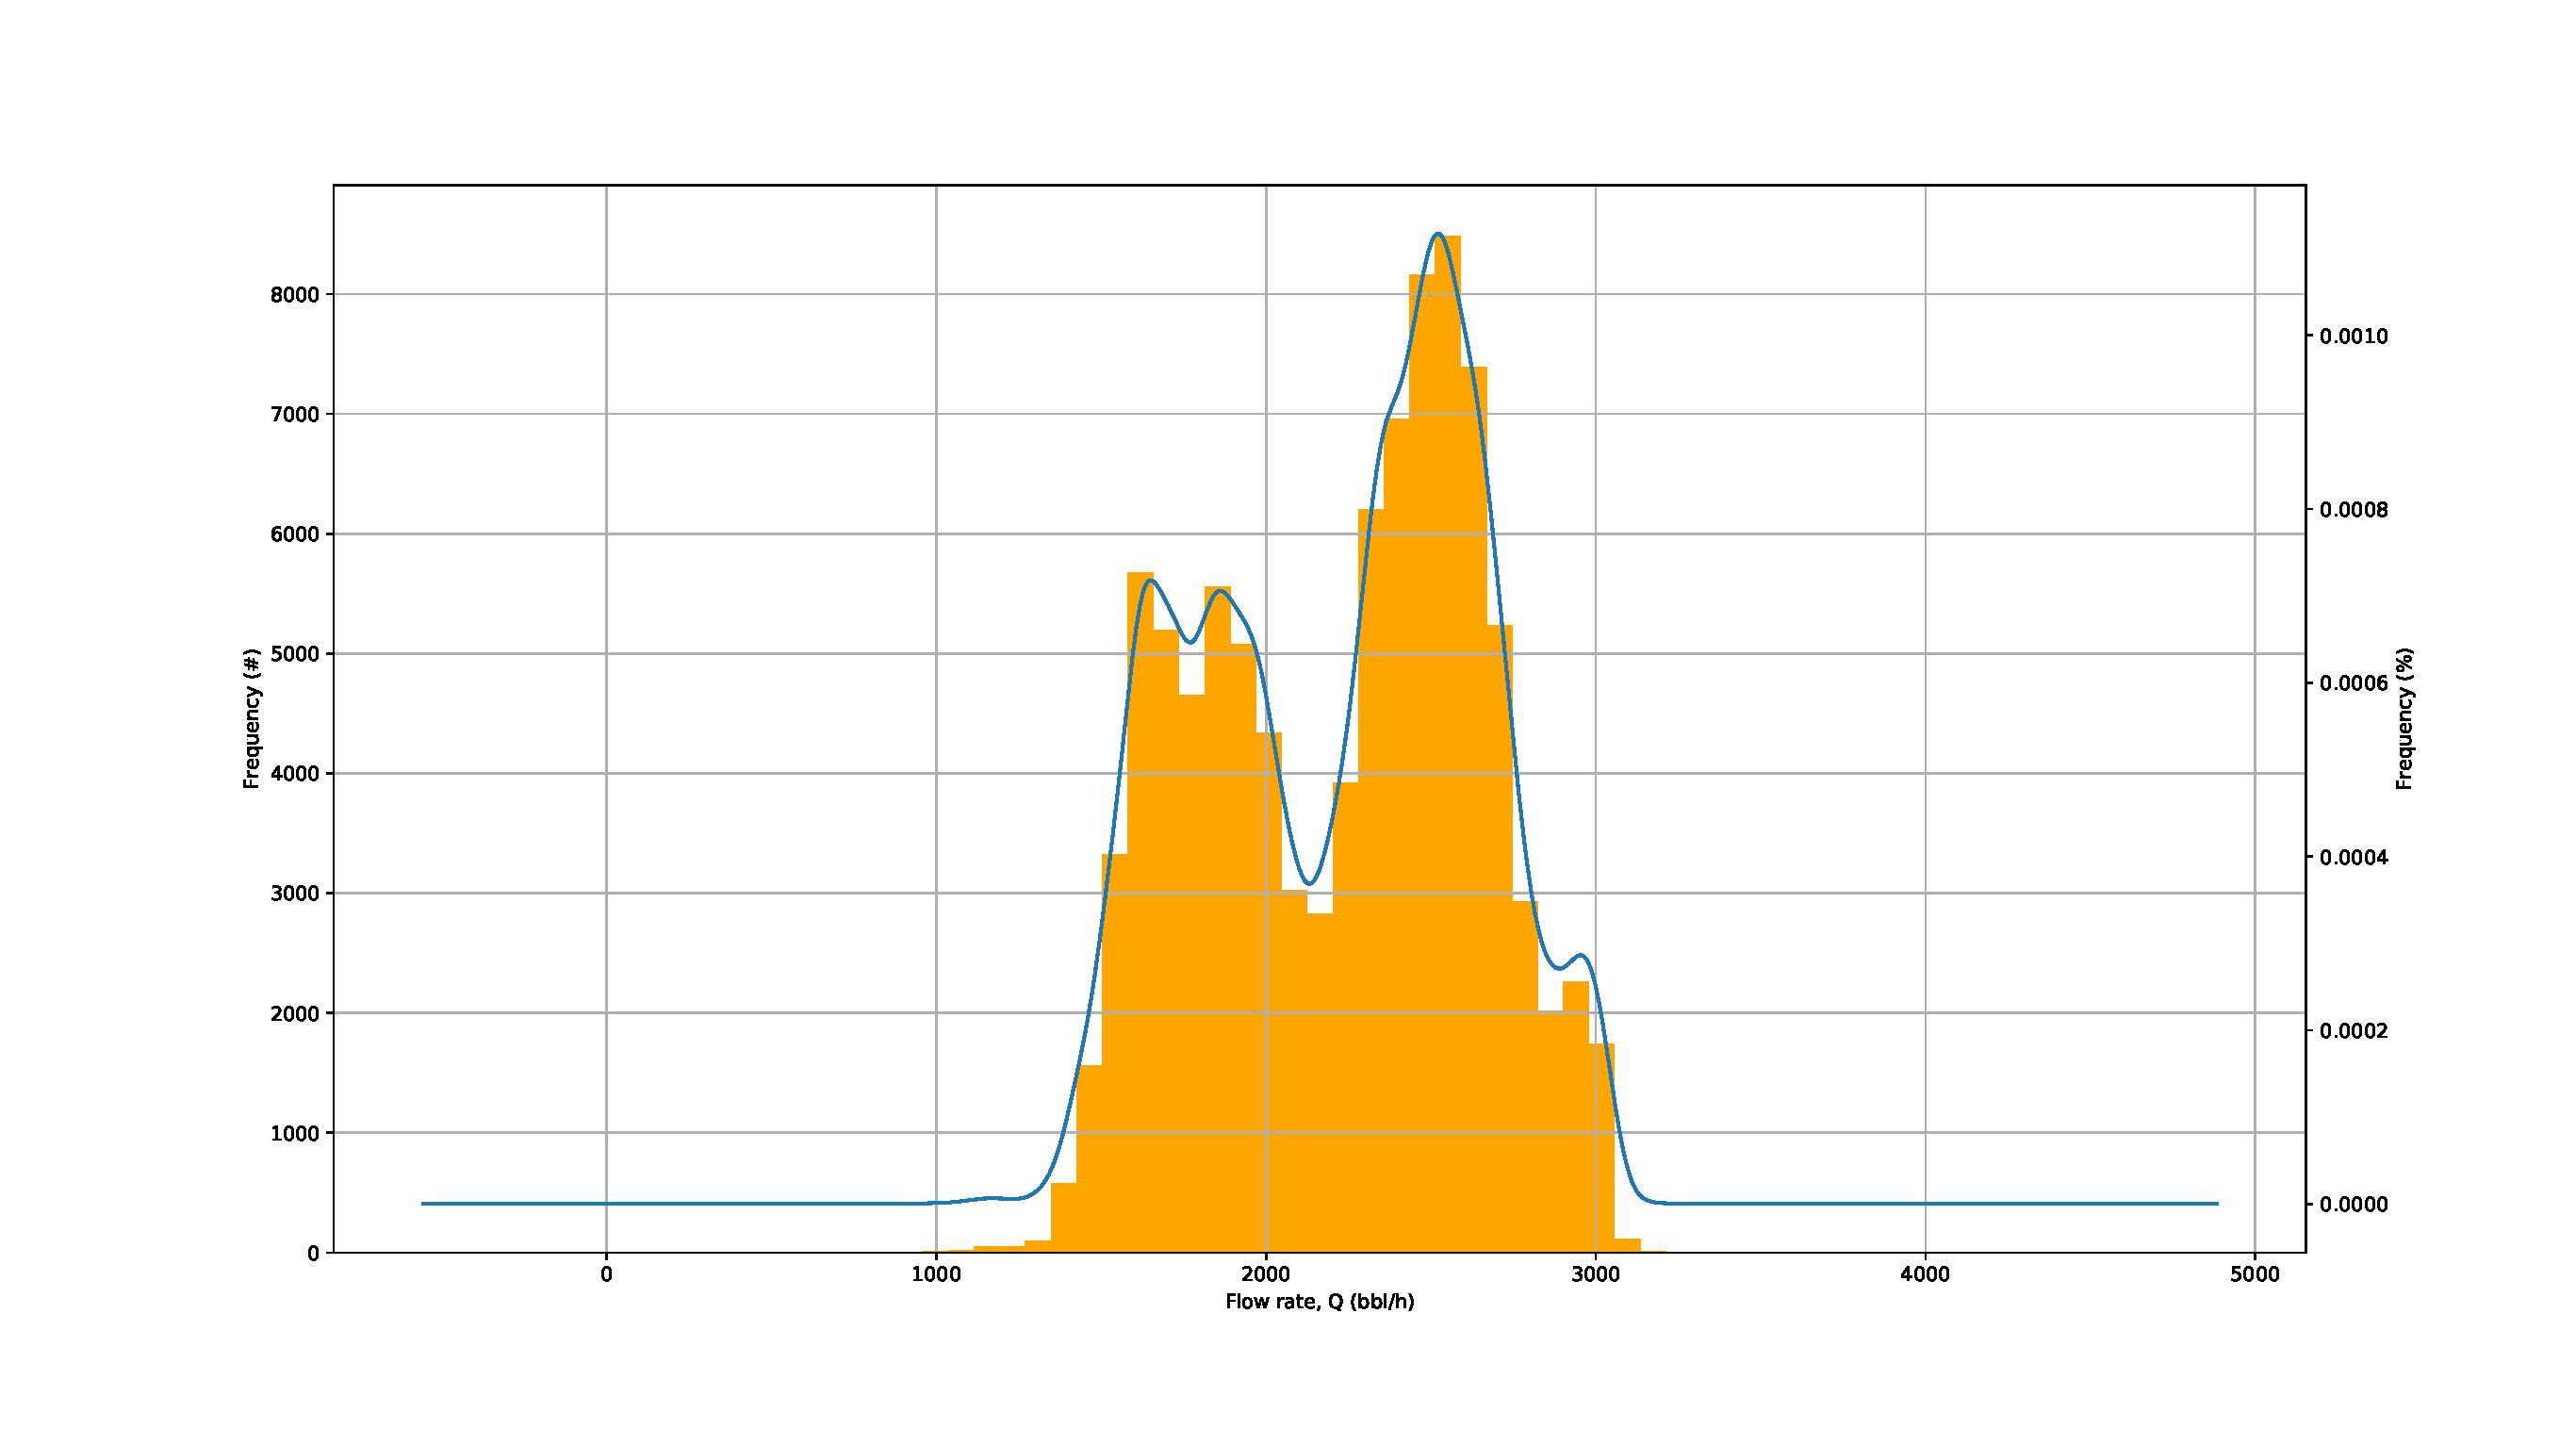
\includegraphics[width=\textwidth]{images/suncor/08Flowrate_KDE.eps}
    \caption{Flow rate distribution of the pre-processed data set.}
    \label{fig:02KDE}
\end{figure}

The segregated distributions created from DBSCAN and the average characteristics of each cluster are shown in Figures \ref{fig:02DBSCAN} and \ref{fig:02DBSCANV}, respectively.  Evidently from Figure \ref{fig:02DBSCANV}, the operation of equipment were vastly different in the two operating regimes.  More specifically, cluster 2 used almost no DRA, and used Station B3 Pump 1 and Station B1 VFD exclusively.  In cluster 1, all equipment were used with exception of Station B3 Pump 1.  From this information, two ML models can be created to cater to each cluster.

\begin{figure}[h]
    \centering
    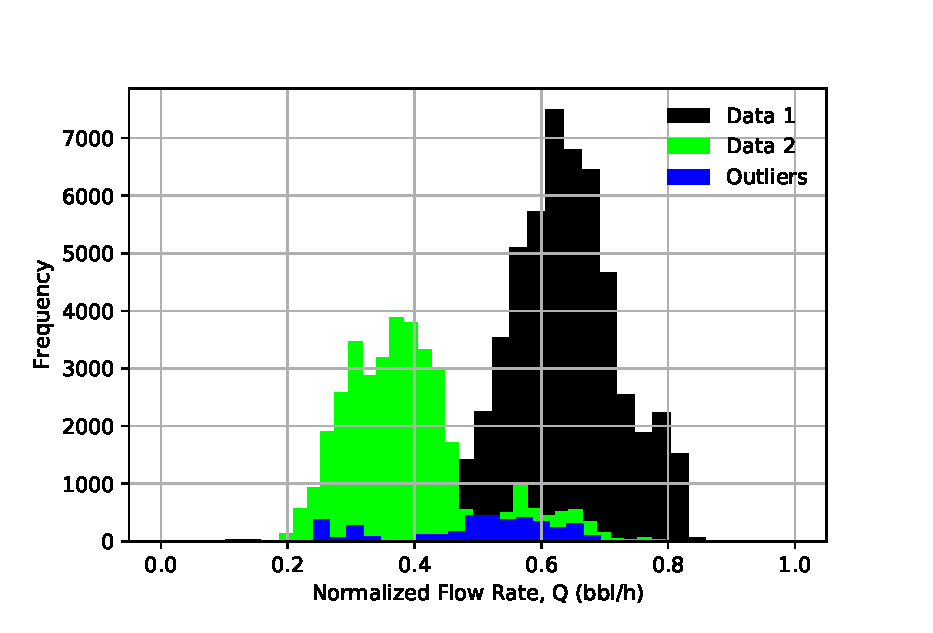
\includegraphics[scale=0.8]{images/suncor/08DBSCAN.eps}
    \caption{Clusters identified after applying the density-based scan.}
    \label{fig:02DBSCAN}
\end{figure}

\begin{figure}[h]
    \centering
    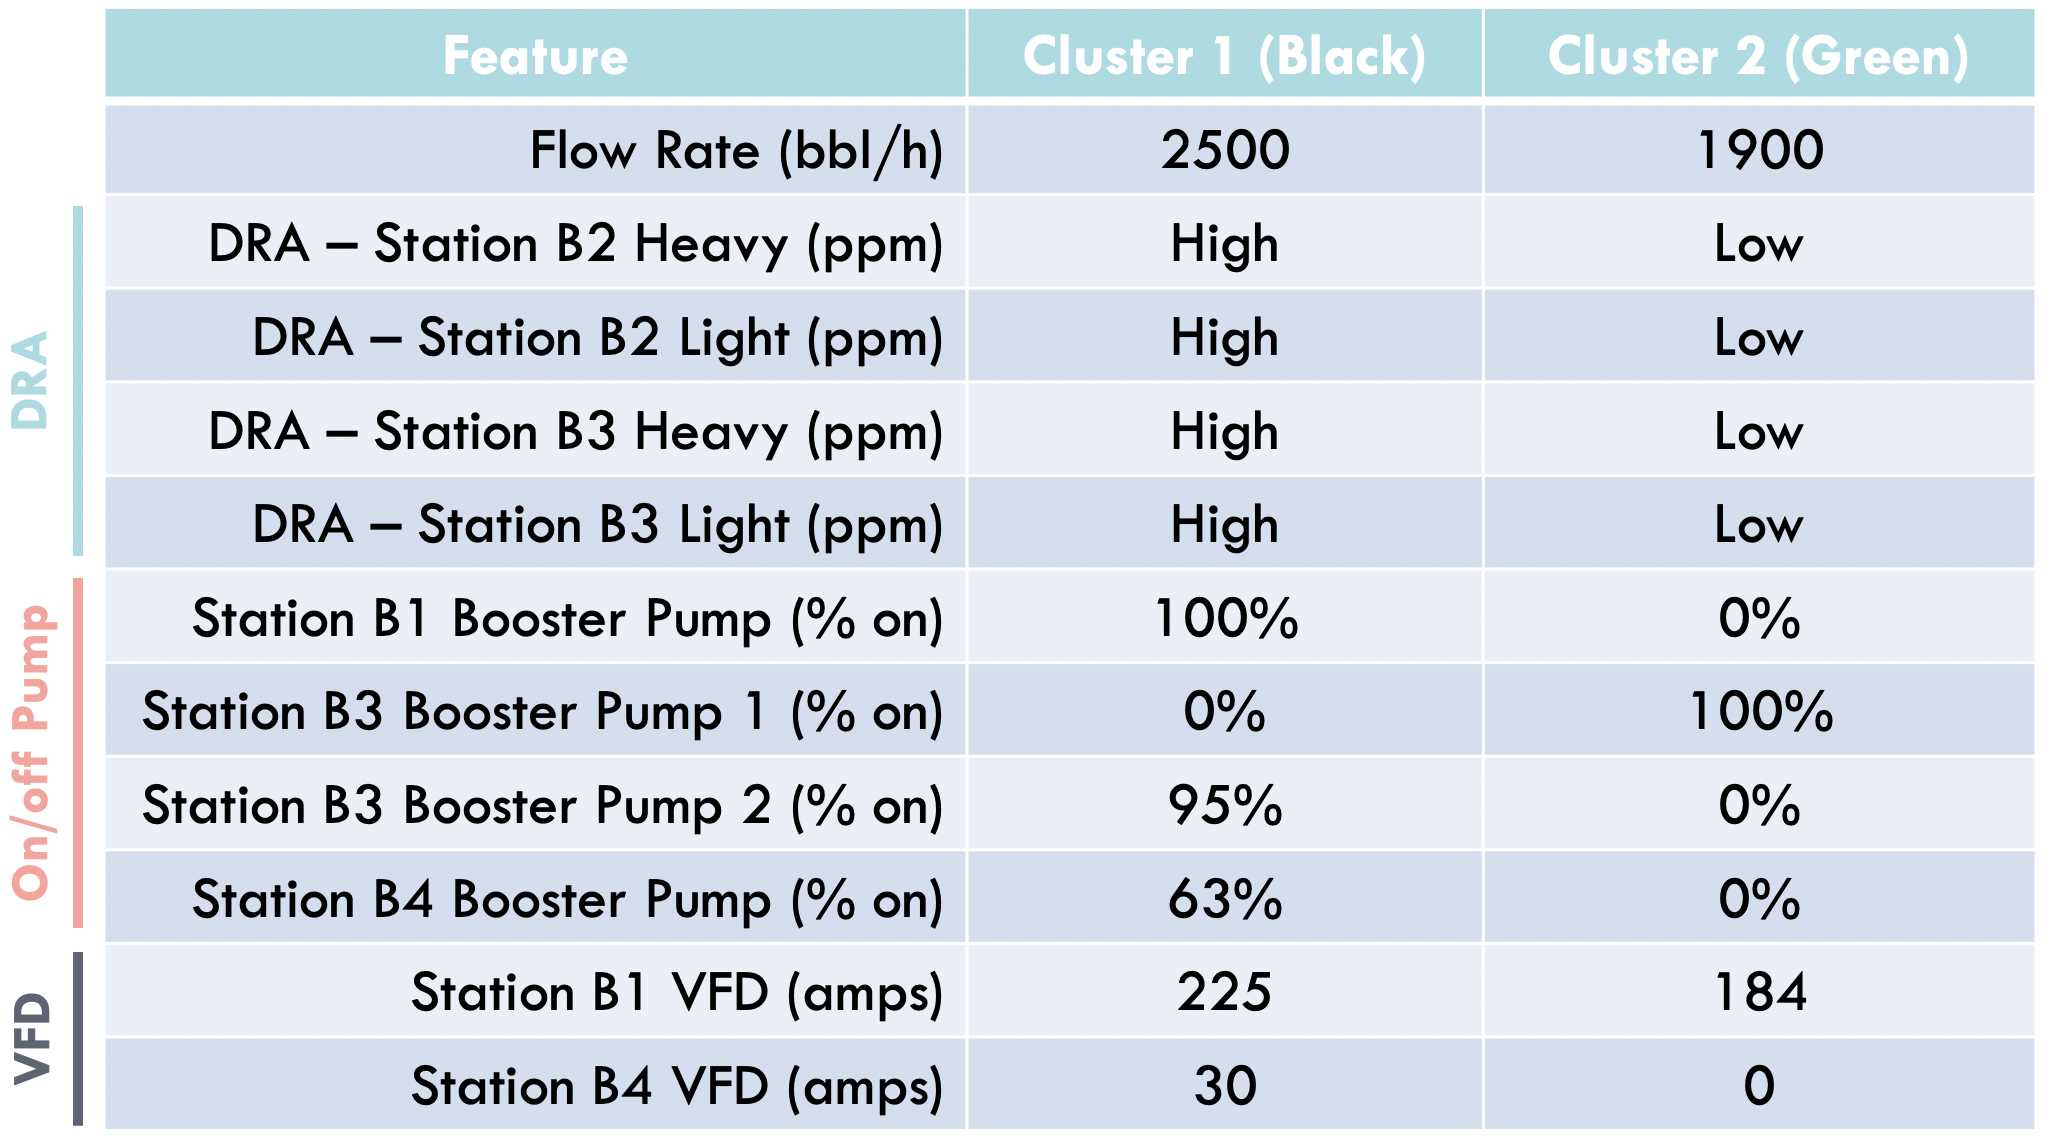
\includegraphics[width=0.8\textwidth]{images/suncor/08AvgChar.jpeg}
    \caption{Average operating variables for the two operating conditions.}
    \label{fig:02DBSCANV}
\end{figure}

\subsection{Machine Learning Predictions}

The following models were implemented to predict for the pipeline outlet flow rate: linear models, polynomial models, neural network models, and LPV models.  Ultimately, the LPV model reigned supreme due to its interpretability, consistent results, simple model structure. The performance and hyper parameters of each model are shown below.  During model identification, the data sets were divided into three sections: training, validation and testing.  Table \ref{tab:02datapart} shows the purpose of each data section.
\begin{table}[h]
    \centering
    {\setstretch{1.2}
    \begin{tabular}{ c | c | p{9cm}}
                            & \% of Data        &  Description \\
        \hline
        Training            &  90\%             
        &  Identify the ML model        \\
        
        Validation          &  5\%              
        &  Tune ML model performance on unseen data         \\
        
        Testing             &  5\%             
        &  Test ML model performance on proxy live data       \\             
    \end{tabular}}
    \caption{Description of each data partition.}
    \label{tab:02datapart}
\end{table}

\subsubsection{Linear Models}
Linear models pertain the simplest model structure and will serve as a benchmark for other models.  The hyper parameters and performance metrics of the model are shown in Table \ref{tab:02LinearHP} and \ref{tab:02LinearPE}, respectively. The model's performance on the validation and test data are shown in Figures \ref{fig:02LSValidation} and \ref{fig:02LSTest}. From \ref{tab:02LinearPE}, the model MAE and RMSE increased 4\% and 6\% on the testing data, respectively.  $R^2$ on the test data significantly reduced.  However, the trends from Figure \ref{fig:02LSTest} does not exhibit any significant inaccuracies. 

\begin{table}[h]
    \centering
    {\setstretch{1.2}
    \begin{tabular}{ c | c}
        Hyper Parameter                  &  Value       \\
        \hline
        Epochs                           &  800      \\
        Minibatch size                   &  8192     \\
        Learning rate, $\alpha$          &  0.001    \\
        Regularization, $\lambda$          &  0.001  \\
    \end{tabular}}
    \caption{Hyper parameters for linear regression.}
    \label{tab:02LinearHP}
\end{table}
\begin{table}[h]
    \centering
    {\setstretch{1.2}
    \begin{tabular}{ c | c | c | c}
                             &  Training data    &  Validation data   &    Test data      \\
        \hline
        MAE                  &  98               &    98              &  102     \\
        RMSE                 &  127              &   127              &  135    \\ 
        $R^2$                &  0.91             &   0.91             &  0.70   \\
    \end{tabular}}
    \caption{Performance assessment for the linear regression.}
    \label{tab:02LinearPE}
\end{table}

\begin{figure}[h]
     \centering
     \begin{subfigure}[b]{0.48\textwidth}
         \centering
         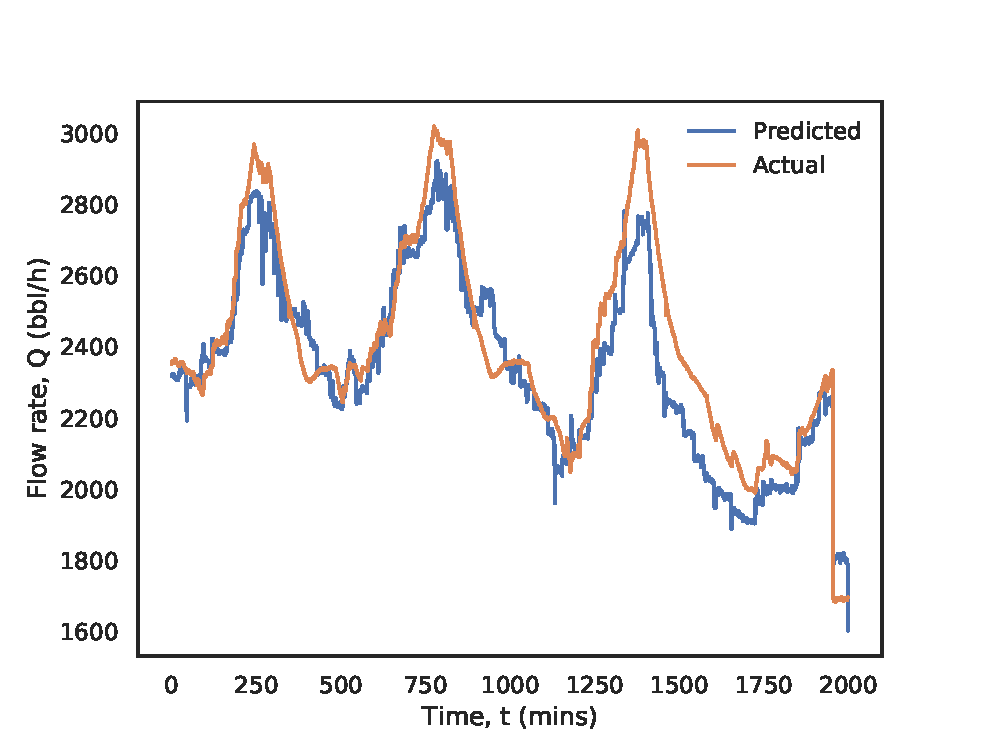
\includegraphics[width=\textwidth]{images/suncor/08ls_validation.eps}
         \caption{Predicted vs. actual flow rate for the validation data set.}
         \label{fig:02LSValidation}
     \end{subfigure}
     \hfill
     \begin{subfigure}[b]{0.48\textwidth}
         \centering
         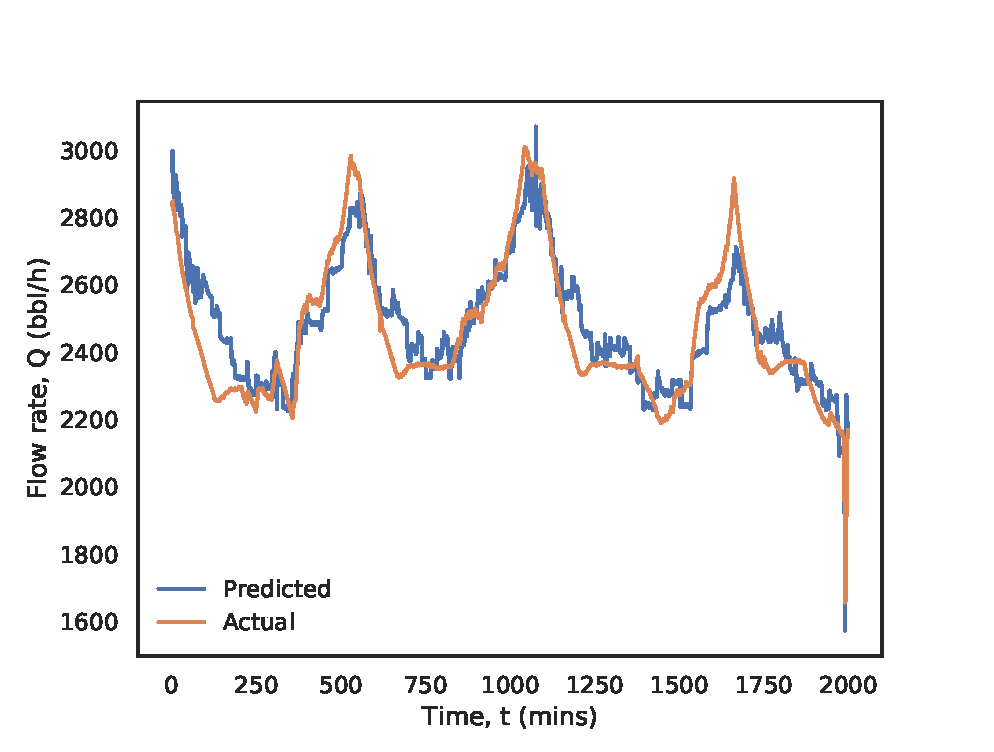
\includegraphics[width=\textwidth]{images/suncor/08ls_test.eps}
         \caption{Predicted vs. actual flow rate for the test data set.}
         \label{fig:02LSTest}
     \end{subfigure}
     \caption{Linear regression validation and test plots.}
        \label{fig:02LSPlots}
\end{figure}

\subsubsection{Polynomial Models}
Non-linear models were used to further enhance predictive capabilities.  Two exponential models were applied: quadratic and square root.  The hyper parameters and performance metrics of the exponential models are shown in Tables \ref{tab:02ExponentialHP} and \ref{tab:02ExponentialHP}, respectively. The model performances on the validation and test data sets is shown in Figure \ref{fig:02PolynomialPlots}. Compared to the benchmark model, the MAE and RMSE decreased by up to 13\% and 15\% on the test data set. Moreover, the model performance does not deteriorate when applied on the test data set. 

\begin{table}[h]
    \centering
    {\setstretch{1.2}
    \begin{tabular}{ c | c | c}
        Hyper Parameter                  &  Quadratic   & Square root       \\
        \hline
        Epochs                           &  1000    & 1000  \\
        Minibatch size                   &  8192    & 8192    \\
        Learning rate, $\alpha$          &  0.001   & 0.001  \\
        Regularization, $\lambda$          &  0.001 & 0.001 \\
    \end{tabular}}
    \caption{Hyper parameters for exponential regression.}
    \label{tab:02ExponentialHP}
\end{table}

\begin{table}[h]
    \centering
    {\setstretch{1.2}
    \begin{tabular}{c|c|c|c|c|c|c|}
      & \multicolumn{2}{c|}{Training data} & \multicolumn{2}{c|}{Validation data} & \multicolumn{2}{c|}{Test data} \\ \cline{2-7} 
      & Quad             & Sqrt            & \multicolumn{1}{c|}{Quad}   & Sqrt   & Quad           & Sqrt          \\ \hline
    MAE   & 92               & 89              & 92                          & 89     & 89             & 91            \\
    RMSE  & 121              & 118             & \multicolumn{1}{c|}{121}    & 117    & 120            & 115           \\
    \end{tabular}}
    \caption{Performance assessment for the quad. and sqrt. model.}
    \label{tab:02ExponentialPE}
\end{table}

\begin{figure}[h]
     \centering
     \begin{subfigure}[b]{0.45\textwidth}
         \centering
         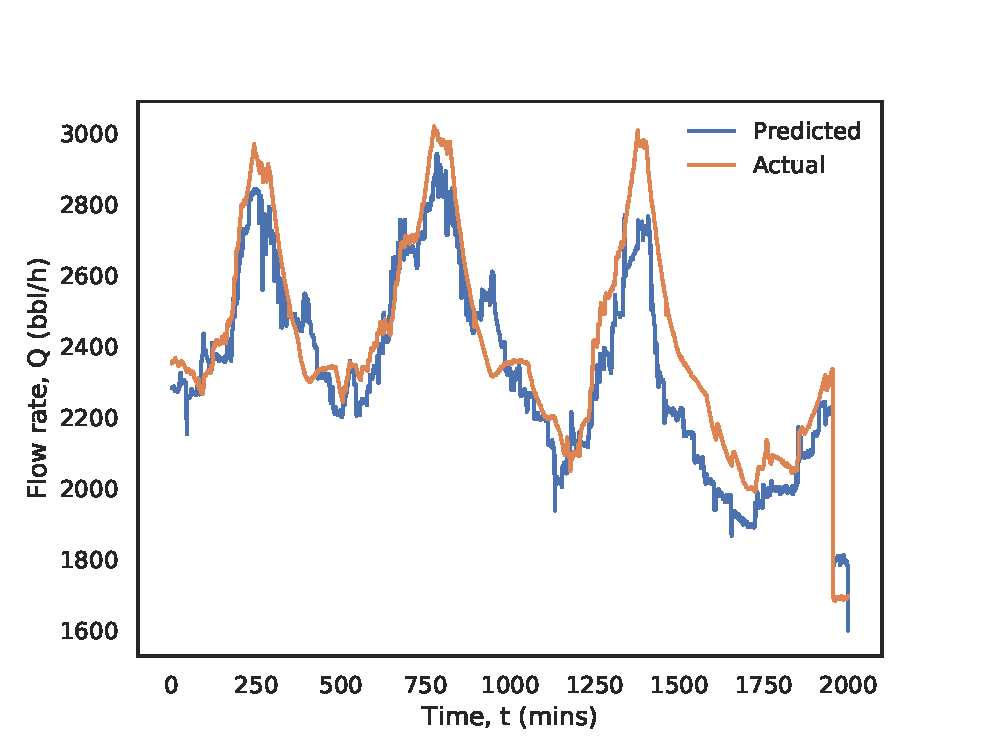
\includegraphics[width=\textwidth]{images/suncor/08quad_validation.eps}
         \caption{Predicted vs. actual flow rate for validation data using the quad. model.}
         \label{fig:02quad_validation}
     \end{subfigure}
     \begin{subfigure}[b]{0.45\textwidth}
         \centering
         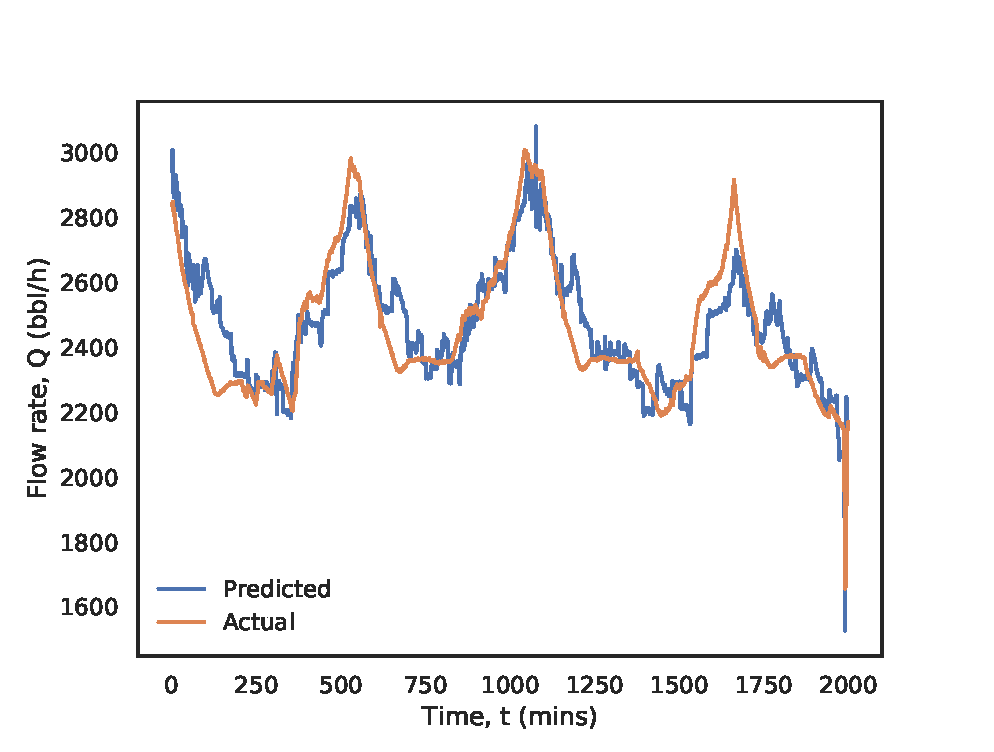
\includegraphics[width=\textwidth]{images/suncor/08quad_test.eps}
         \caption{Predicted vs. actual flow rate for the test data using the quadratic model.}
         \label{fig:02quad_test}
     \end{subfigure}
     \begin{subfigure}[b]{0.45\textwidth}
         \centering
         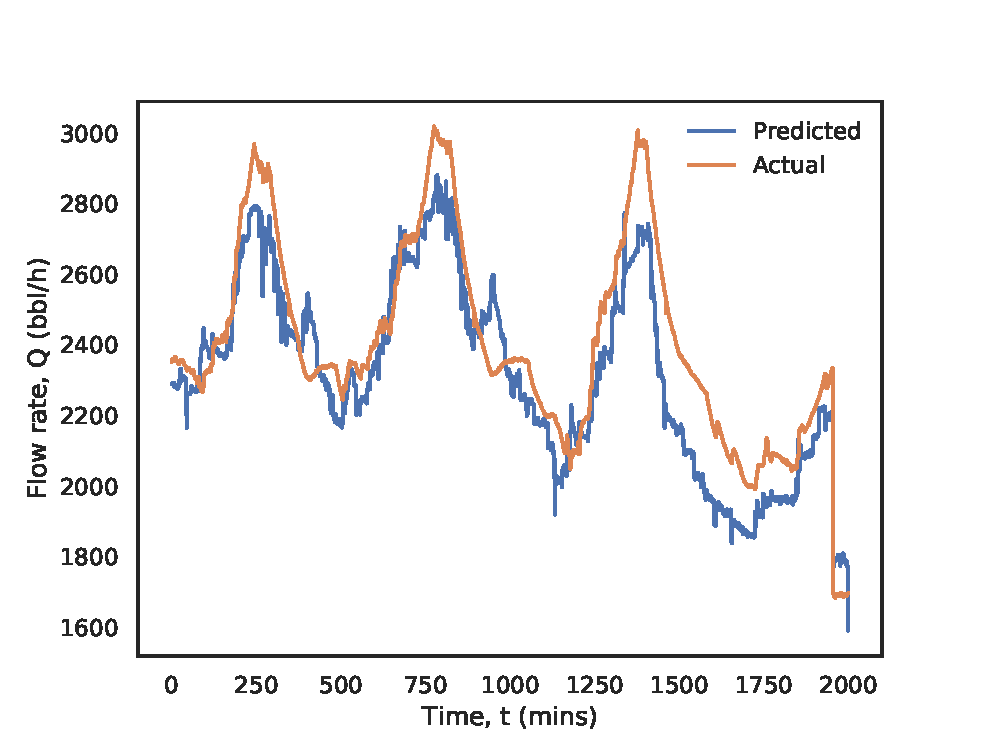
\includegraphics[width=\textwidth]{images/suncor/08sqrt_validation.eps}
         \caption{Predicted vs. actual flow rate for the validation data using the sqrt. model.}
         \label{fig:02sqrt_validation}
     \end{subfigure}
     \begin{subfigure}[b]{0.45\textwidth}
         \centering
         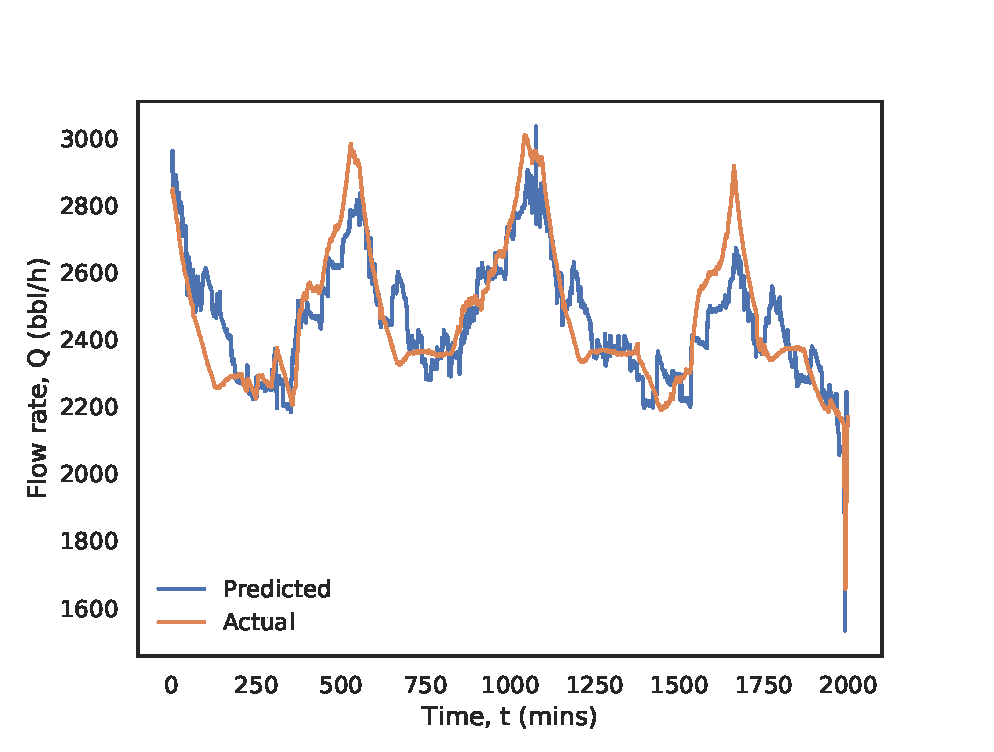
\includegraphics[width=\textwidth]{images/suncor/08sqrt_test.eps}
         \caption{Predicted vs. actual flow rate for the test data using the sqrt. model.}
         \label{fig:02sqrt_test}
     \end{subfigure}
        \caption{Polynomial regression validation and test plots.}
        \label{fig:02PolynomialPlots}
\end{figure}

\subsubsection{Neural Network Models}
Neural networks and deep learning were the most advanced models to be applied to this prediction task.  Here, three different neural networks with varying sizes were trained and their performances evaluated. 

Tables \ref{tab:02NNHP} and \ref{tab:02NNPE} show the hyper parameters and performance metrics of the three neural networks.  Figure \ref{fig:02NNPlots} shows the neural networks' performance on the validation and test data sets.  From Table \ref{tab:02NNPE}, it is clear that the training and validation error decreased as the neural network increased in size; however, the errors increased significantly on the test data. This was caused by the test data being different than the training data.  In this particular case, the test data was collected in the summer months where temperatures increased by up to $\ang{10}$ C compared to the training data.  Because of the complexity and parameterization of neural network models, data even slightly different from the training data can have a significant impact on accuracy.  Smaller, simpler, more regularized neural network models could be used to avoid this behaviour. Indeed, it can be seen that the test data error increased as the size of the network increased. Another disadvantage of neural networks are its lack of interpretability.  Investigating the effects of each regressor in this highly non-linear model is nearly impossible; hence, neural networks are black box models and might be undesirable for safety critical systems.
\begin{table}[h]
    \centering
    {\setstretch{1.2}
    \begin{tabular}{ c | c | c | c}
        Hyper Parameter                            &  Small NN  &  Med. NN  & Large NN       \\
        \hline
        Epochs                                     &  700       & 1000      & 1200  \\
        Minibatch size                             &  8192      & 8192      & 8192  \\
        Learning rate, $\alpha$                    &  0.001     & 0.001     & 0.001 \\
        Regularization, $\lambda$                  &  0.001     & 0.003     & 0.005 \\
        Number of layers                           &  3         & 6         & 8     \\
        Neurons per layer                          &  20        & 30        & 40    \\
        Activation function for hidden layers      & ReLU       & ReLU      & ReLU  \\
        Activation function for hidden layers      & Linear     & Linear    & Linear \\
    \end{tabular}}
    \caption{Hyper parameters for the feed-forward neural network.}
    \label{tab:02NNHP}
\end{table}

\begin{table}[h]
\centering
{\setstretch{1.2}
\begin{tabular}{c|c|c|c|c|c|c|c|c|c|}
\multicolumn{1}{l|}{} & \multicolumn{3}{c|}{Training Data}                                               & \multicolumn{3}{c|}{Validation Data}                                             & \multicolumn{3}{c|}{Test Data}                                                   \\ \cline{2-10} 
\multicolumn{1}{l|}{} & \multicolumn{1}{c|}{Sm.} & \multicolumn{1}{c|}{Med.} & \multicolumn{1}{c|}{Lar.} & \multicolumn{1}{c|}{Sm.} & \multicolumn{1}{c|}{Med.} & \multicolumn{1}{c|}{Lar.} & \multicolumn{1}{c|}{Sm.} & \multicolumn{1}{c|}{Med.} & \multicolumn{1}{c|}{Lar.} \\ \hline
MAE                   & 48                       & 42                        & 38                        & 50                       & 45                        & 37                        & 87                       & 87                        & 91                        \\
RMSE                  & 66                       & 58                        & 57                        & 69                       & 61                        & 56                        & 107                      & 117                       & 118                       \\
\end{tabular}}
    \caption{Performance assessment of the neural network models.}
    \label{tab:02NNPE}
\end{table}

\begin{figure}[p]
     \centering
     \begin{subfigure}[b]{0.48\textwidth}
         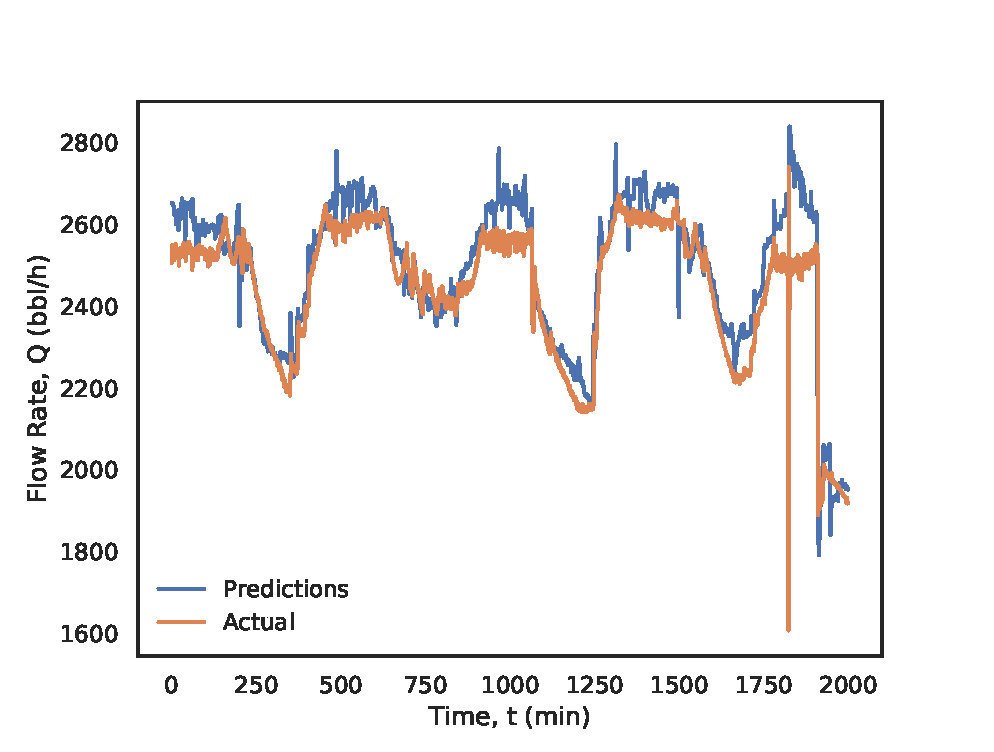
\includegraphics[width=\textwidth]{images/suncor/08smallnn_valid.eps}
         \caption{Validation data for the small neural net.}
         \label{fig:02smallnn_valid}
     \end{subfigure}
     \begin{subfigure}[b]{0.48\textwidth}
         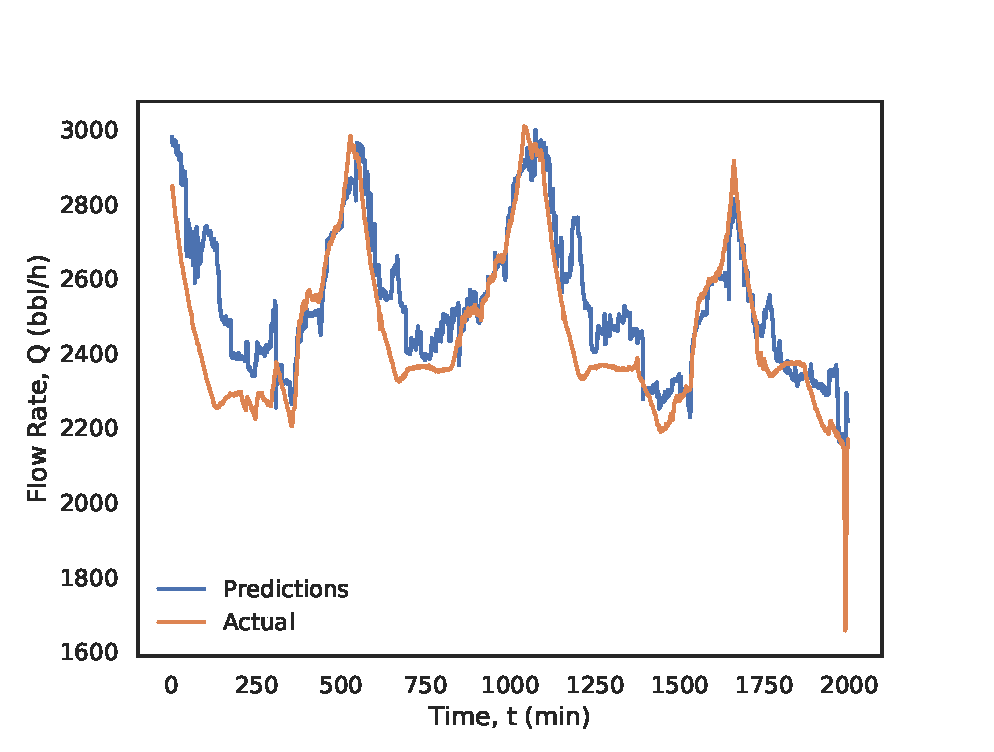
\includegraphics[width=\textwidth]{images/suncor/08smallnn_test.eps}
         \caption{Test data for the small neural net.}
         \label{fig:02smallnn_test}
     \end{subfigure}
     \begin{subfigure}[b]{0.48\textwidth}
         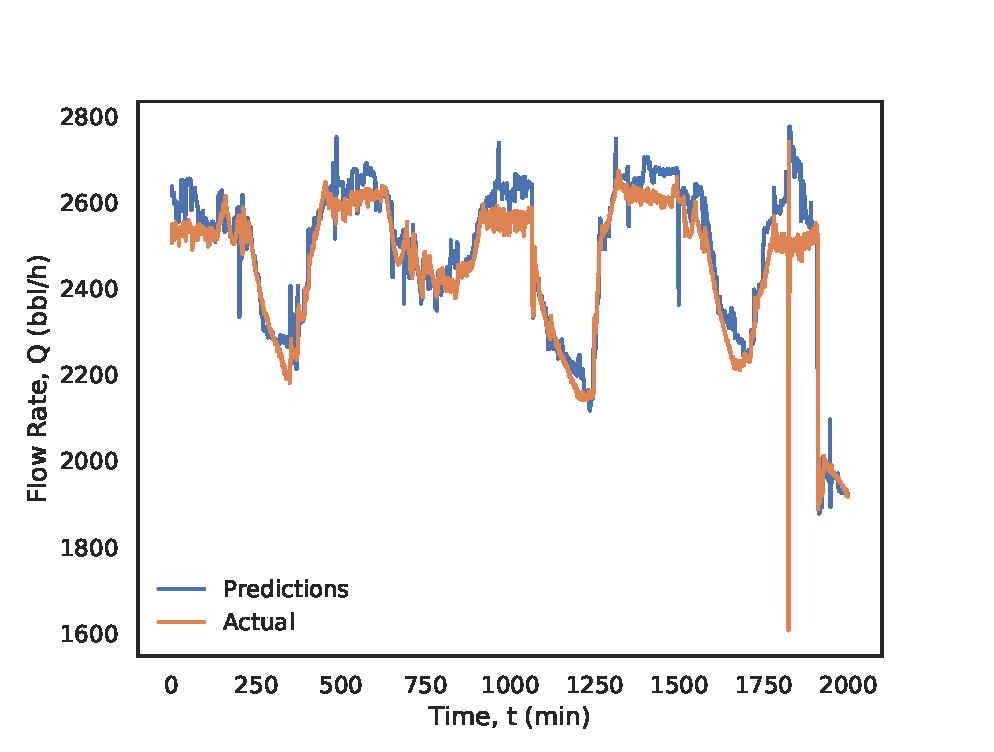
\includegraphics[width=\textwidth]{images/suncor/08mednn_valid.eps}
         \caption{Validation data for the med. neural net.}
         \label{fig:02mednn_valid}
     \end{subfigure}
     \begin{subfigure}[b]{0.48\textwidth}
         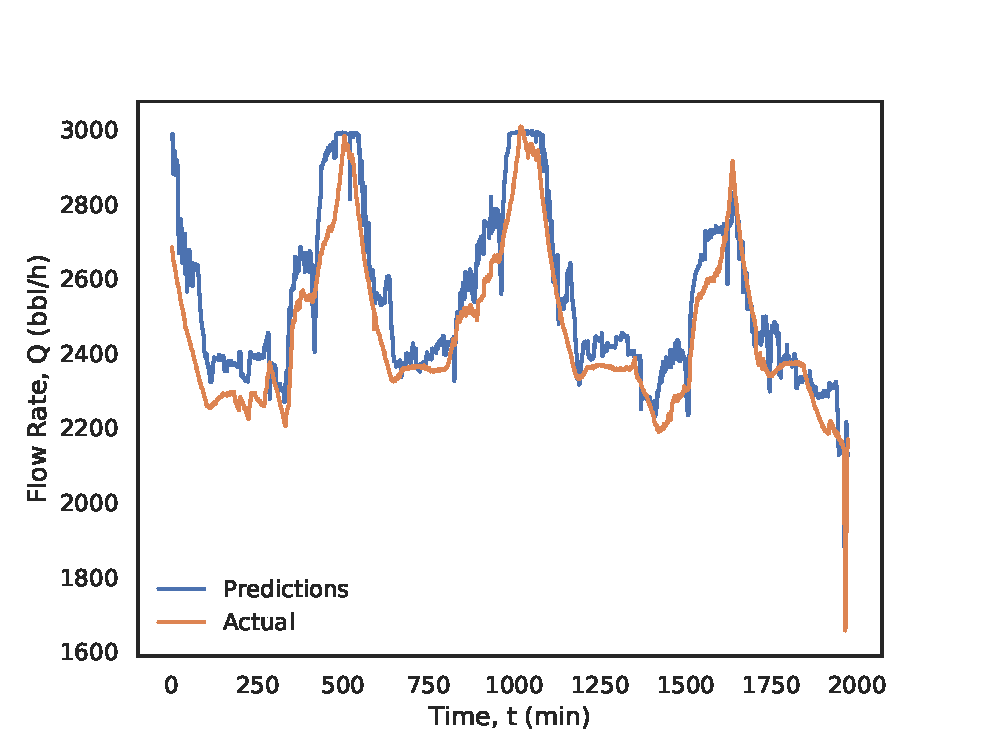
\includegraphics[width=\textwidth]{images/suncor/08mednn_test.eps}
         \caption{Test data for the med. neural net.}
         \label{fig:02mednn_test}
     \end{subfigure}
     \begin{subfigure}[b]{0.48\textwidth}
         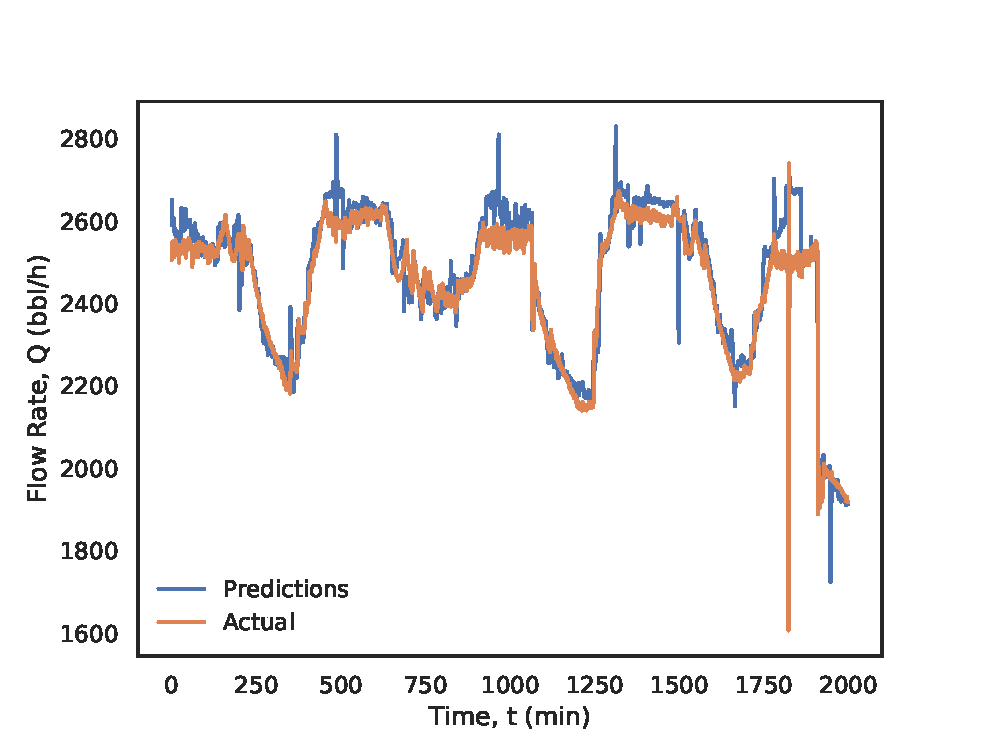
\includegraphics[width=\textwidth]{images/suncor/08largenn_valid.eps}
         \caption{Validation data for the large neural net.}
         \label{fig:02largenn_valid}
     \end{subfigure}
     \begin{subfigure}[b]{0.48\textwidth}
         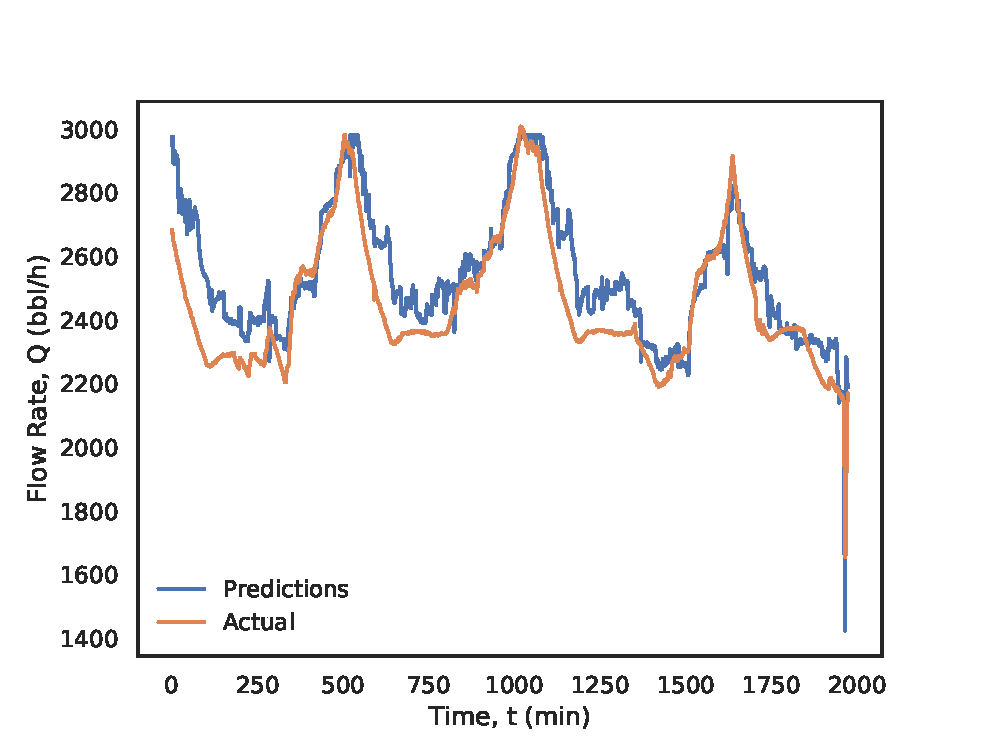
\includegraphics[width=\textwidth]{images/suncor/08largenn_test.eps}
         \caption{Test data for the large neural net.}
         \label{fig:02largenn_test}
     \end{subfigure}
        \caption{Predicted vs. actual flow rates for the feed-forward neural networks.}
        \label{fig:02NNPlots}
\end{figure}


\subsubsection{Linear Parameter-varying Models}
Linear parameter-varying models achieve the performance of non-linear models using a system of linear models.  Furthermore, the models are fully interpretable through its weights.  From the author's experience, this model structure is an ideal starting point for most industrial applications.  For this project, two linear model were identified; one for each cluster in Figure \ref{fig:02DBSCAN}.

The hyper parameters for each linear model is identical to the values shown in Table \ref{tab:02LinearHP}. Performance metrics of the two linear models are shown in Table \ref{tab:02LPVPE}.  The model performance on the validation and test data sets are shown in Figure \ref{fig:02LPVPlots}. Average MAE and RMSE of the LPV model is nearly identical to the square root models (the best non-linear model).  Moreover, the linear models are simpler and have unique regressors in each model.  For example, the linear model for cluster 2 is only a function of the Station B1 VFD current and the DRA ppms because all other inputs did not change in the data set.  Visually, the performance figures show low correlation; however, this is because the validation and test data sets were different compared to the previous models since the data set had to be decomposed.  Additionally, the flow rate in these new data sets contain higher noise compared to previous data and the y-axis range is also reduced, enhancing the noise. Ultimately, the performance metrics illustrate that the performance of the LPV model is nearly identical to the non-linear models and was the model of choice in this industrial application.

\begin{table}[h]
    \centering
    {\setstretch{1.2}
    \begin{tabular}{c|c|c|c|c|c|c|}
      & \multicolumn{2}{c|}{Training data} & \multicolumn{2}{c|}{Validation data} & \multicolumn{2}{c|}{Test data} \\ \cline{2-7} 
      & Cl. 1            & Cl. 2           & Cl. 1             & Cl. 2            & Cl. 1          & Cl. 2         \\ \hline
    MAE   & 90               & 66              & 90                & 67               & 96             & 85            \\
    RMSE  & 115              & 91              & 116               & 92               & 120            & 110           \\
    $R^2$ & 0.87             & 0.90            & 0.86              & 0.89             & 0.78           & 0.57         
    \end{tabular}}
    \caption{Performance assessment for clusters 1 and 2 regression models.}
    \label{tab:02LPVPE}
\end{table}

\begin{figure}[h]
    \centering
     \begin{subfigure}[b]{0.48\textwidth}
         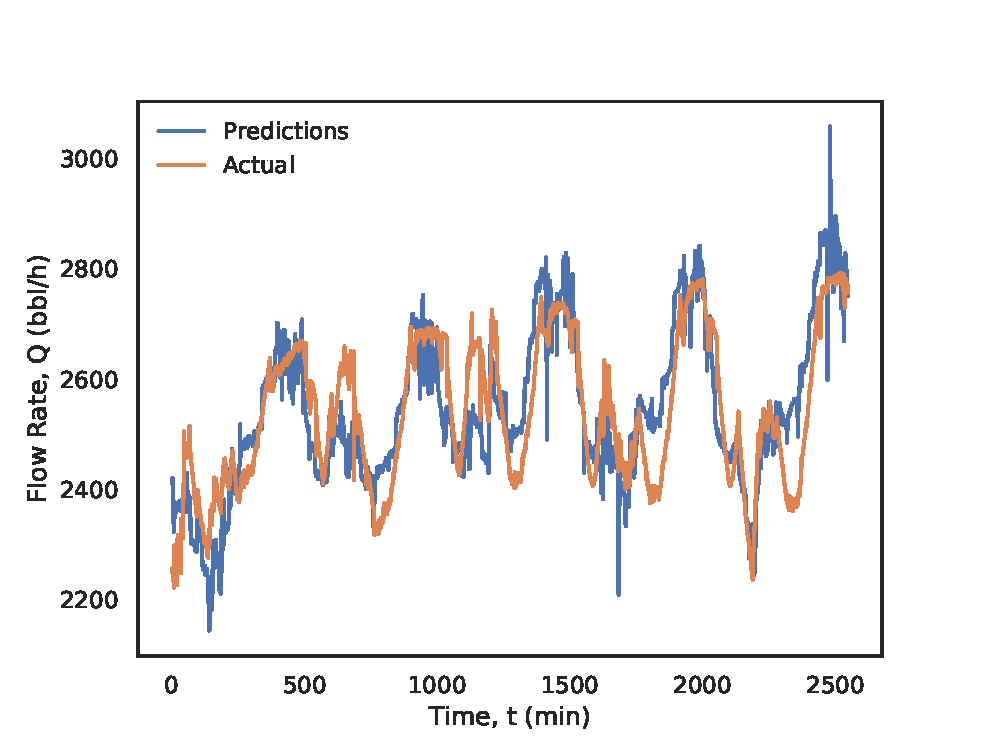
\includegraphics[width=\textwidth]{images/suncor/08cluster1_valid.eps}
         \caption{Validation data using model 1.}
         \label{fig:02cluster1_valid}
     \end{subfigure}
     \begin{subfigure}[b]{0.48\textwidth}
         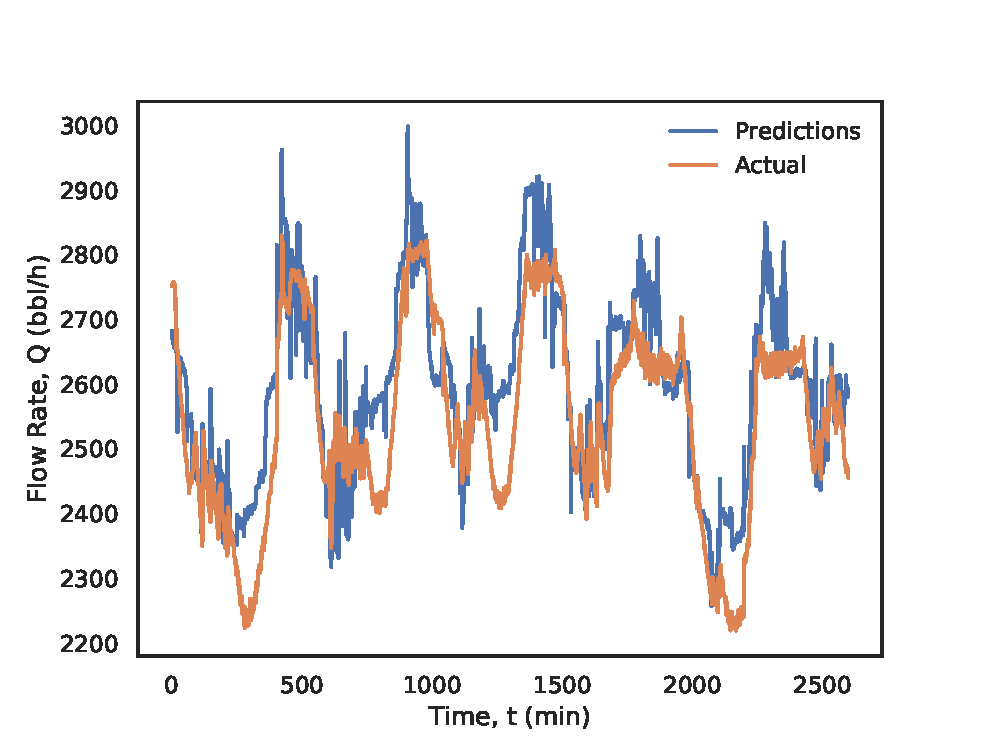
\includegraphics[width=\textwidth]{images/suncor/08cluster1_test.eps}
         \caption{Test data using model 1.}
         \label{fig:02cluster1_test}
     \end{subfigure}
     \begin{subfigure}[b]{0.48\textwidth}
         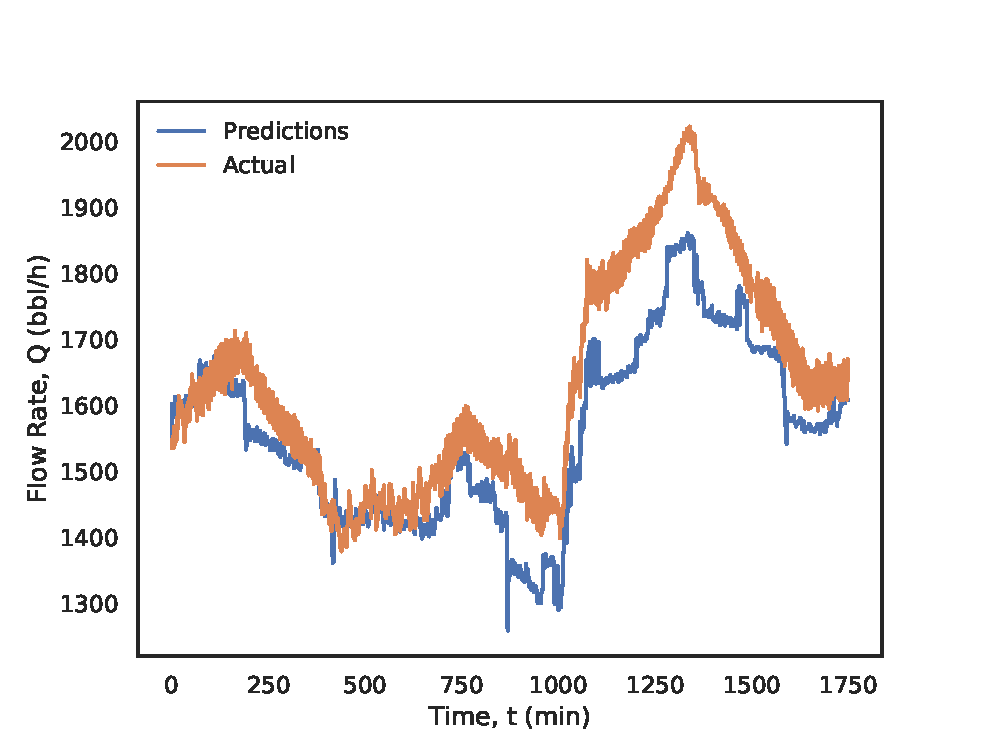
\includegraphics[width=\textwidth]{images/suncor/08cluster2_valid.eps}
         \caption{Validation data using model 2.}
         \label{fig:02cluster2_valid}
     \end{subfigure}
     \begin{subfigure}[b]{0.48\textwidth}
         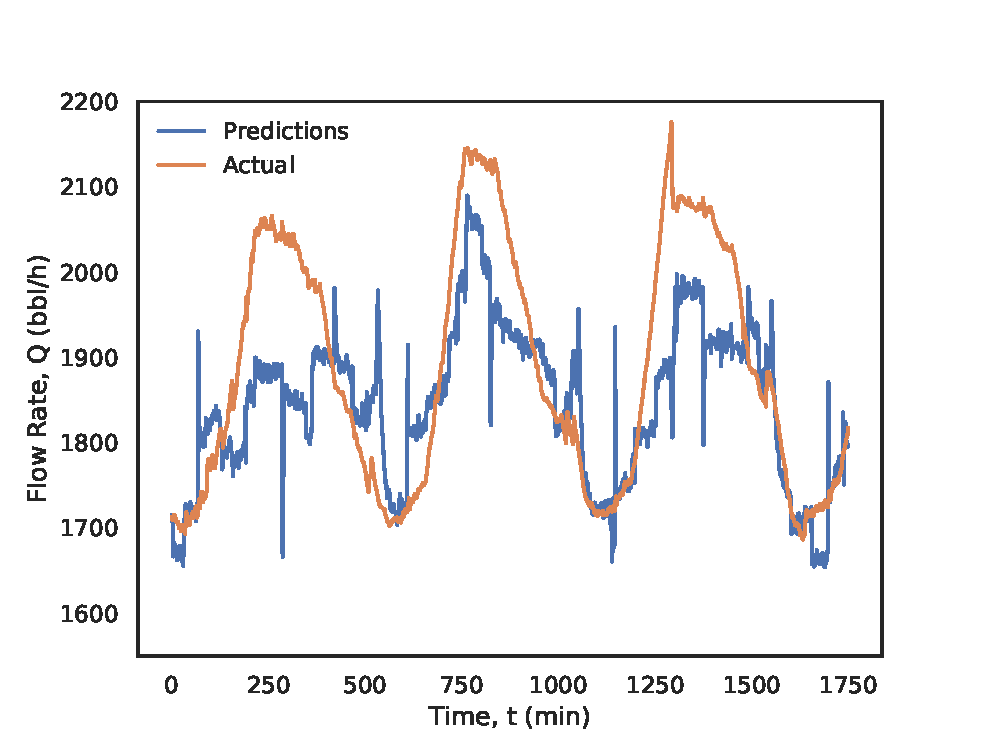
\includegraphics[width=\textwidth]{images/suncor/08cluster2_test.eps}
         \caption{Test data using model 2.}
         \label{fig:02cluster2_test}
     \end{subfigure}
        \caption{Predicted vs. actual flow rate for the linear parameter-varying models.}
        \label{fig:02LPVPlots}
\end{figure}

\subsection{Implementation of USIS}
After the model accuracy was deemed acceptable by the industrial sponsors, the next phase of the project aimed to automate machine learning updates, creating a true self-learning system.  The USIS algorithm was applied to automate each update step, while avoiding outliers and catastrophic interference. 

The hyper parameters for USIS are summarized in Table \ref{tab:02USISHP}. The model was set to update every 24 hours to avoid any significant changes in model weights. Each update step has a maximum of 1440 ($24 \times 60)$ data points per bin. There were ten bins for each model; each had a width of 200 bbl/h.  The bins ranged from 1200 - 3200 bbl/h.  The Euclidean distance was used to calculate the distance metric, $d$.  Moreover, the neglect parameter was selected to be 1.13, identical to $\epsilon$.  Finally, the replay buffer kept the last three months data in memory to avoid catastrophic interference.  Three months was recommended by the industrial sponsors to .

\begin{table}[h]
    \centering
    \begin{tabular}{c|c}
    Hyper parameter & Value \\ \hline
    \# of models, $n$ & 2 \\
    Model update frequency & 24 hrs \\
    Bin size, (bbl/h) & 200 \\
    Distance metric, $d$ & Euclidean \\
    Neglect parameter, $\eta$ & 1.13 \\
    Replay buffer & 129,600 (3 months) \\
    \end{tabular}
    \caption{USIS hyper parameters for the pipeline project.}
    \label{tab:02USISHP}
\end{table}

The overall USIS algorithm implemented onto the industrial pipeline is shown in Figure \ref{fig:02USISPipe}.

\begin{figure}
    \centering
    \includegraphics[width=\textwidth]{}
    \caption{An overall look at the USIS algorithm on the industrial pipeline}
    \label{fig:02USISPipe}
\end{figure}
